\chapter{Additional plots}

This appendix contains additional plots documenting various stages of the analysis which were not fully reported in the main body of the thesis to ease the reading process. 

\section{Background estimation plots}

Figures \ref{fig:kNN_minima_MMT}, \ref{fig:kNN_minima_EMT}, and \ref{fig:kNN_minima_EET} show the \chisq scans as a function of the number of neighbors employed in the classifier as described in Section \ref{sec:kNN_uncertainties} for the 8 TeV datasets of $\mu\mu\tau_h$, $e\mu\tau_h$, and $ee\tau_h$ channels, respectively. 

Figures \ref{fig:fake_rate_mmt}, \ref{fig:fake_rate_emt}, and \ref{fig:fake_rate_eet} show the measured fake rate for the corresponding datasets as a function of the kNN training variables.

\begin{figure}
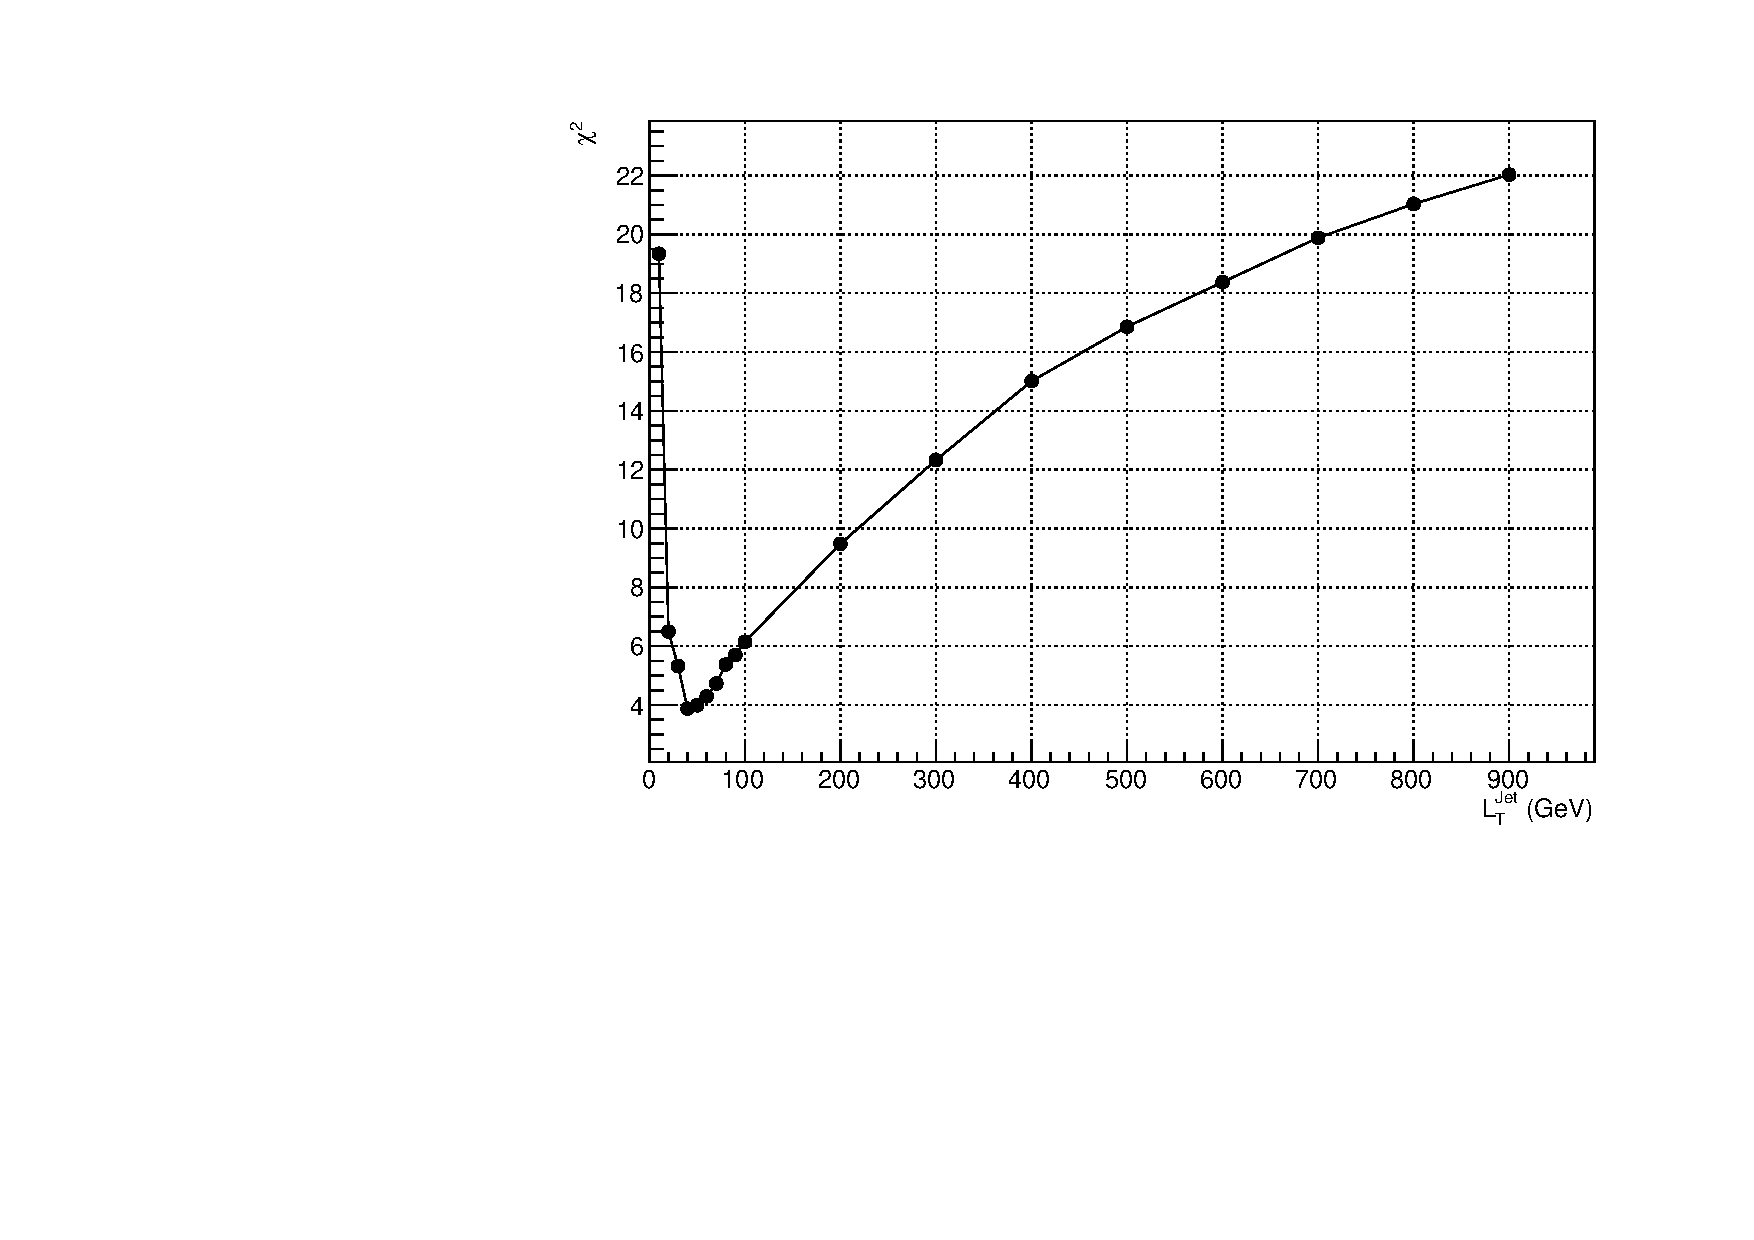
\includegraphics[width=0.5\textwidth]{4_Analisys/pics/8TeV/ProfileNeighbors/MM/h2taucuts/LT_chi2.pdf}
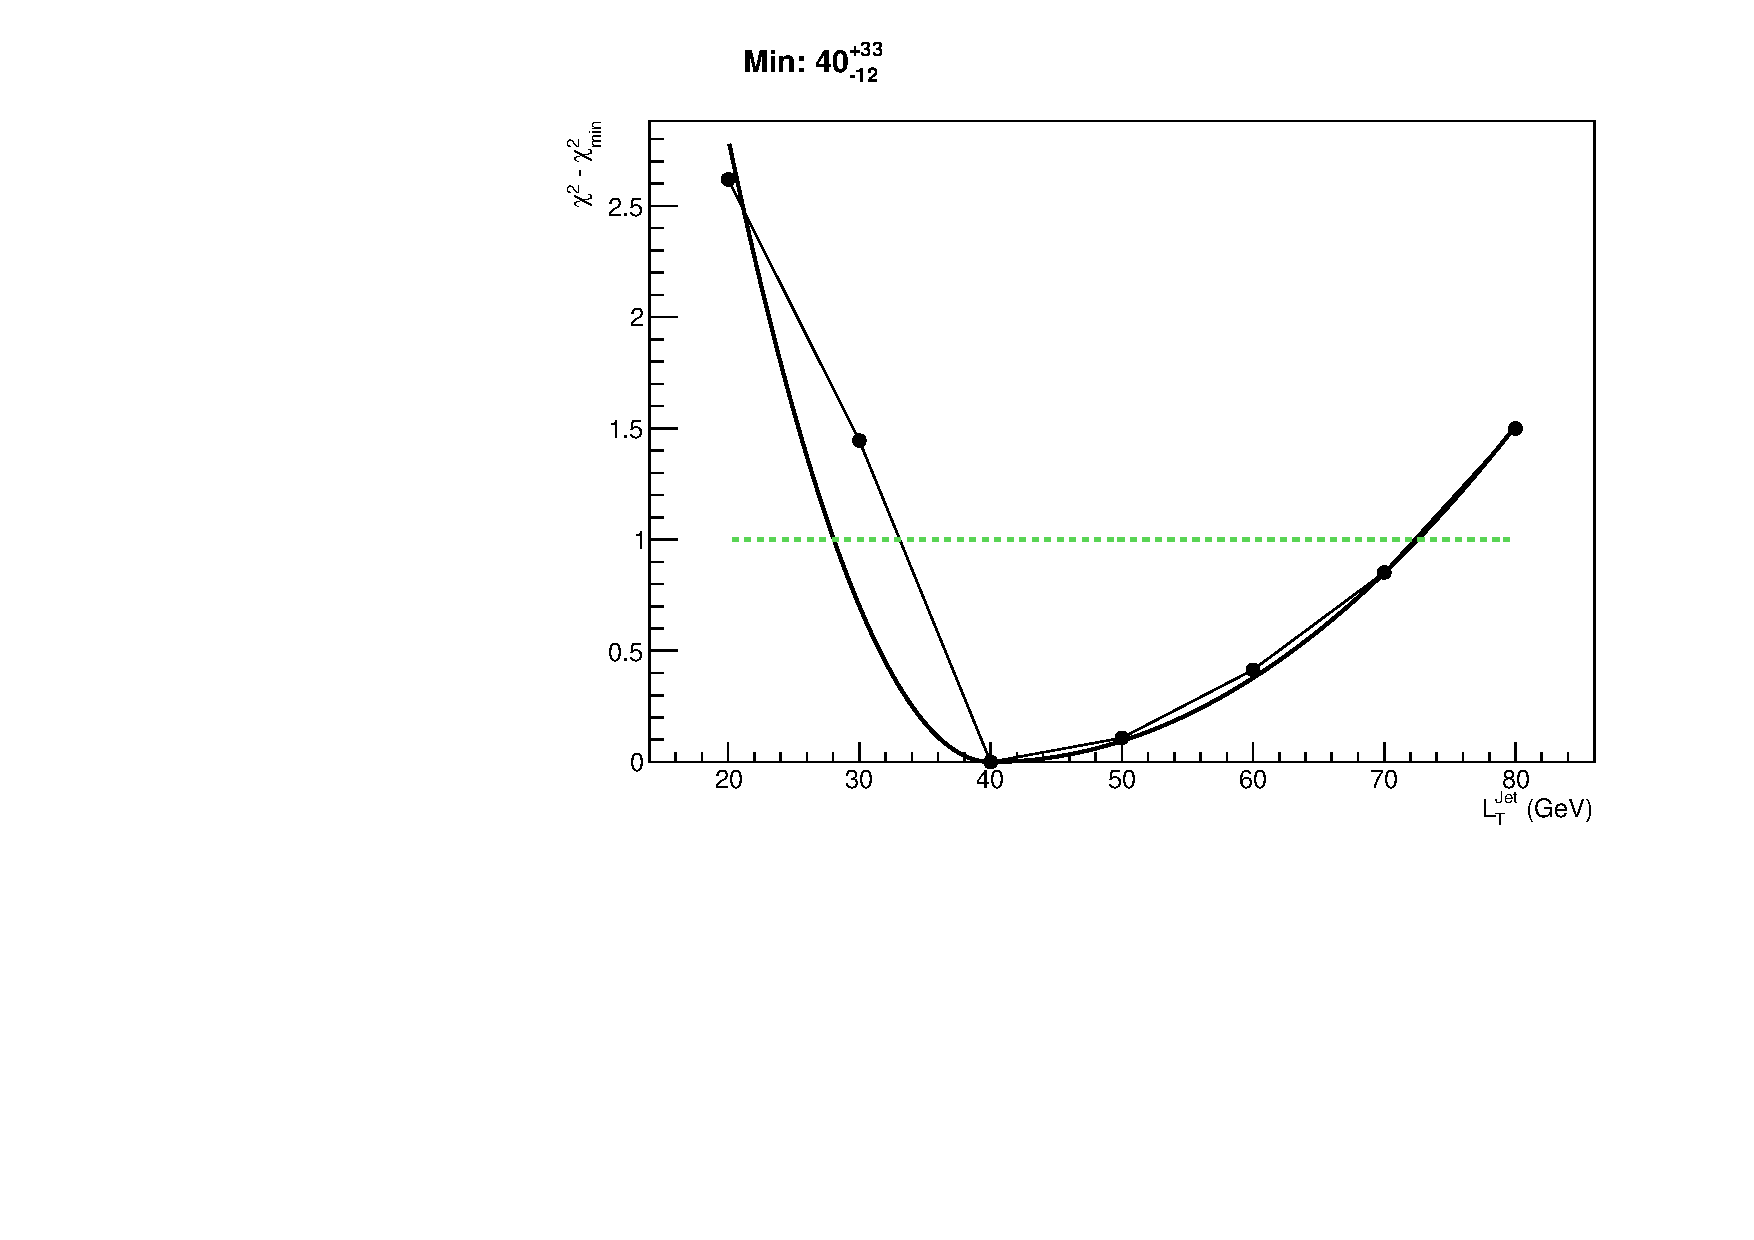
\includegraphics[width=0.5\textwidth]{4_Analisys/pics/8TeV/ProfileNeighbors/MM/h2taucuts_LT.pdf} \\
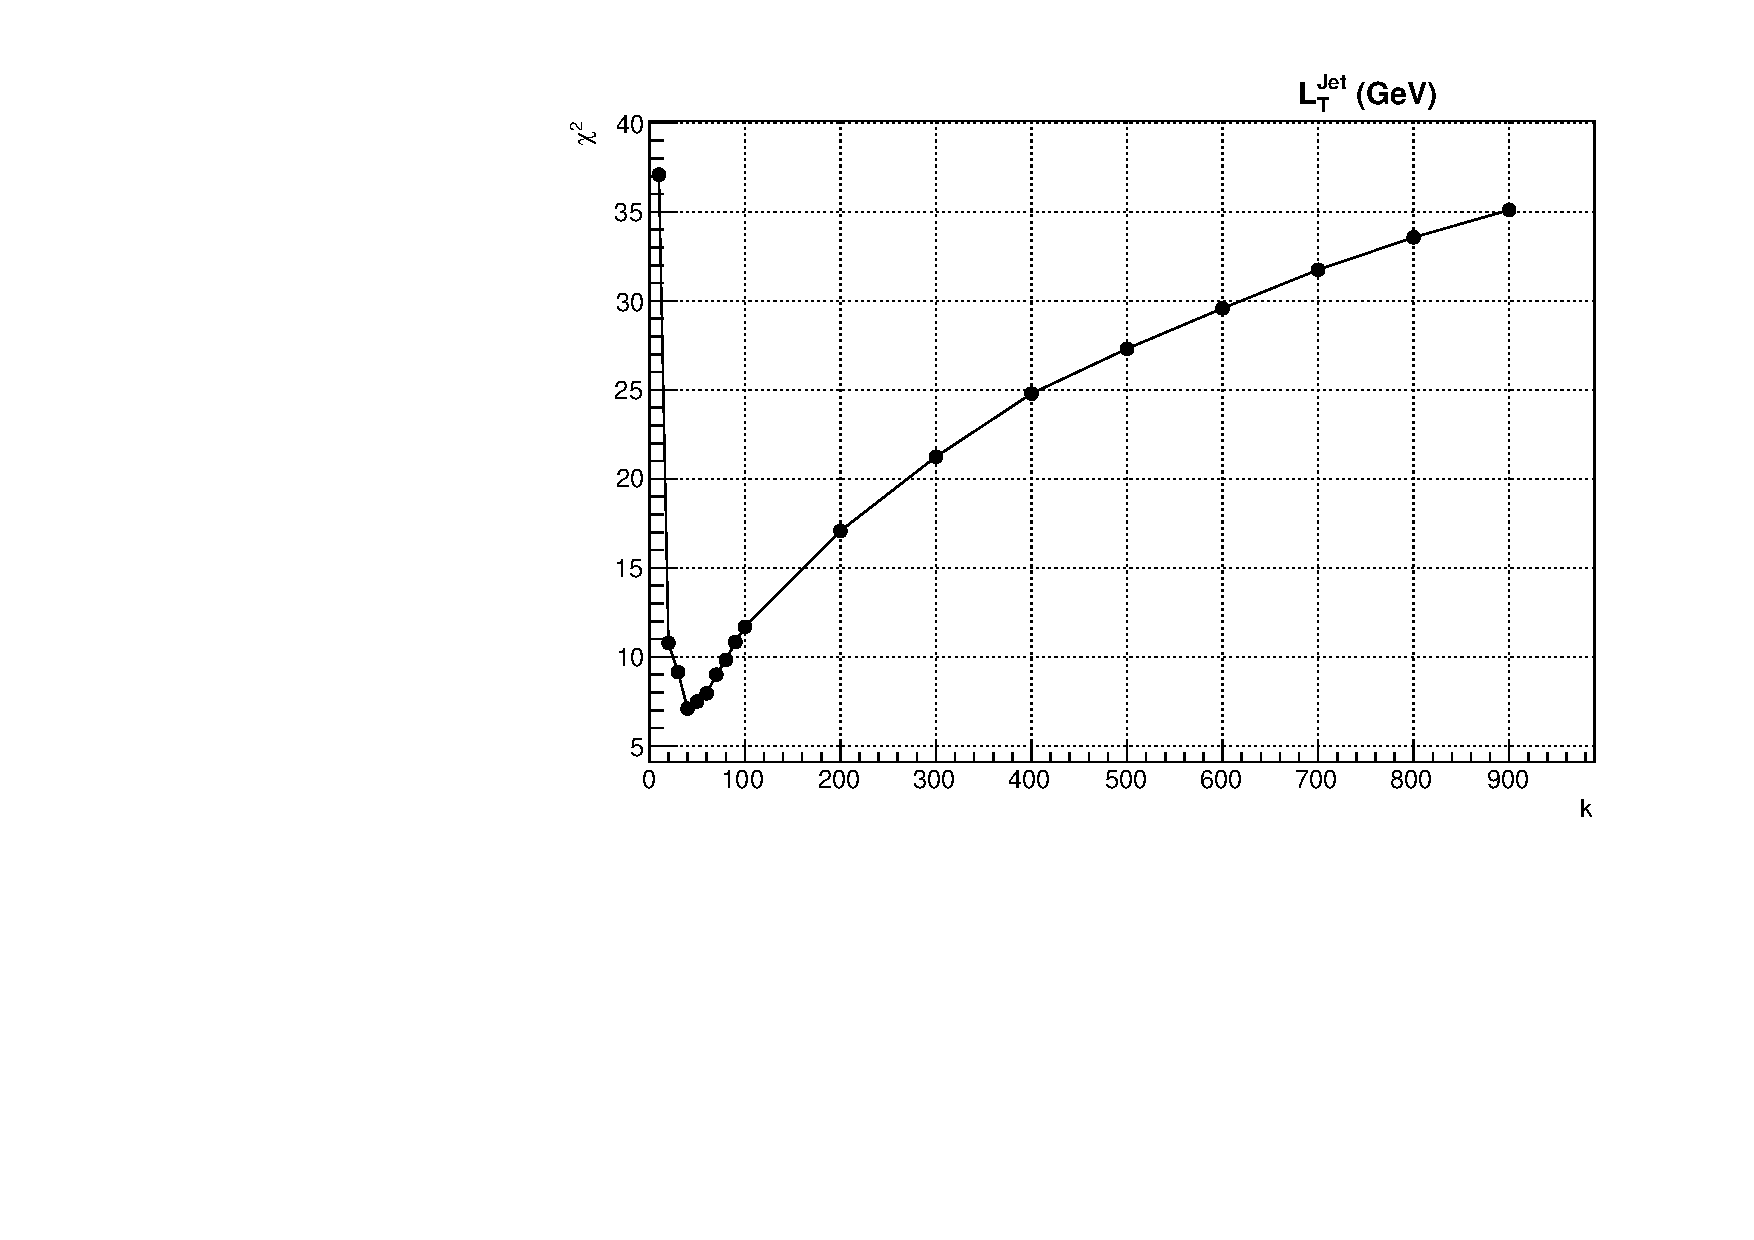
\includegraphics[width=0.5\textwidth]{4_Analisys/pics/8TeV/ProfileNeighbors/MM/h2taucuts020/LT_chi2.pdf}
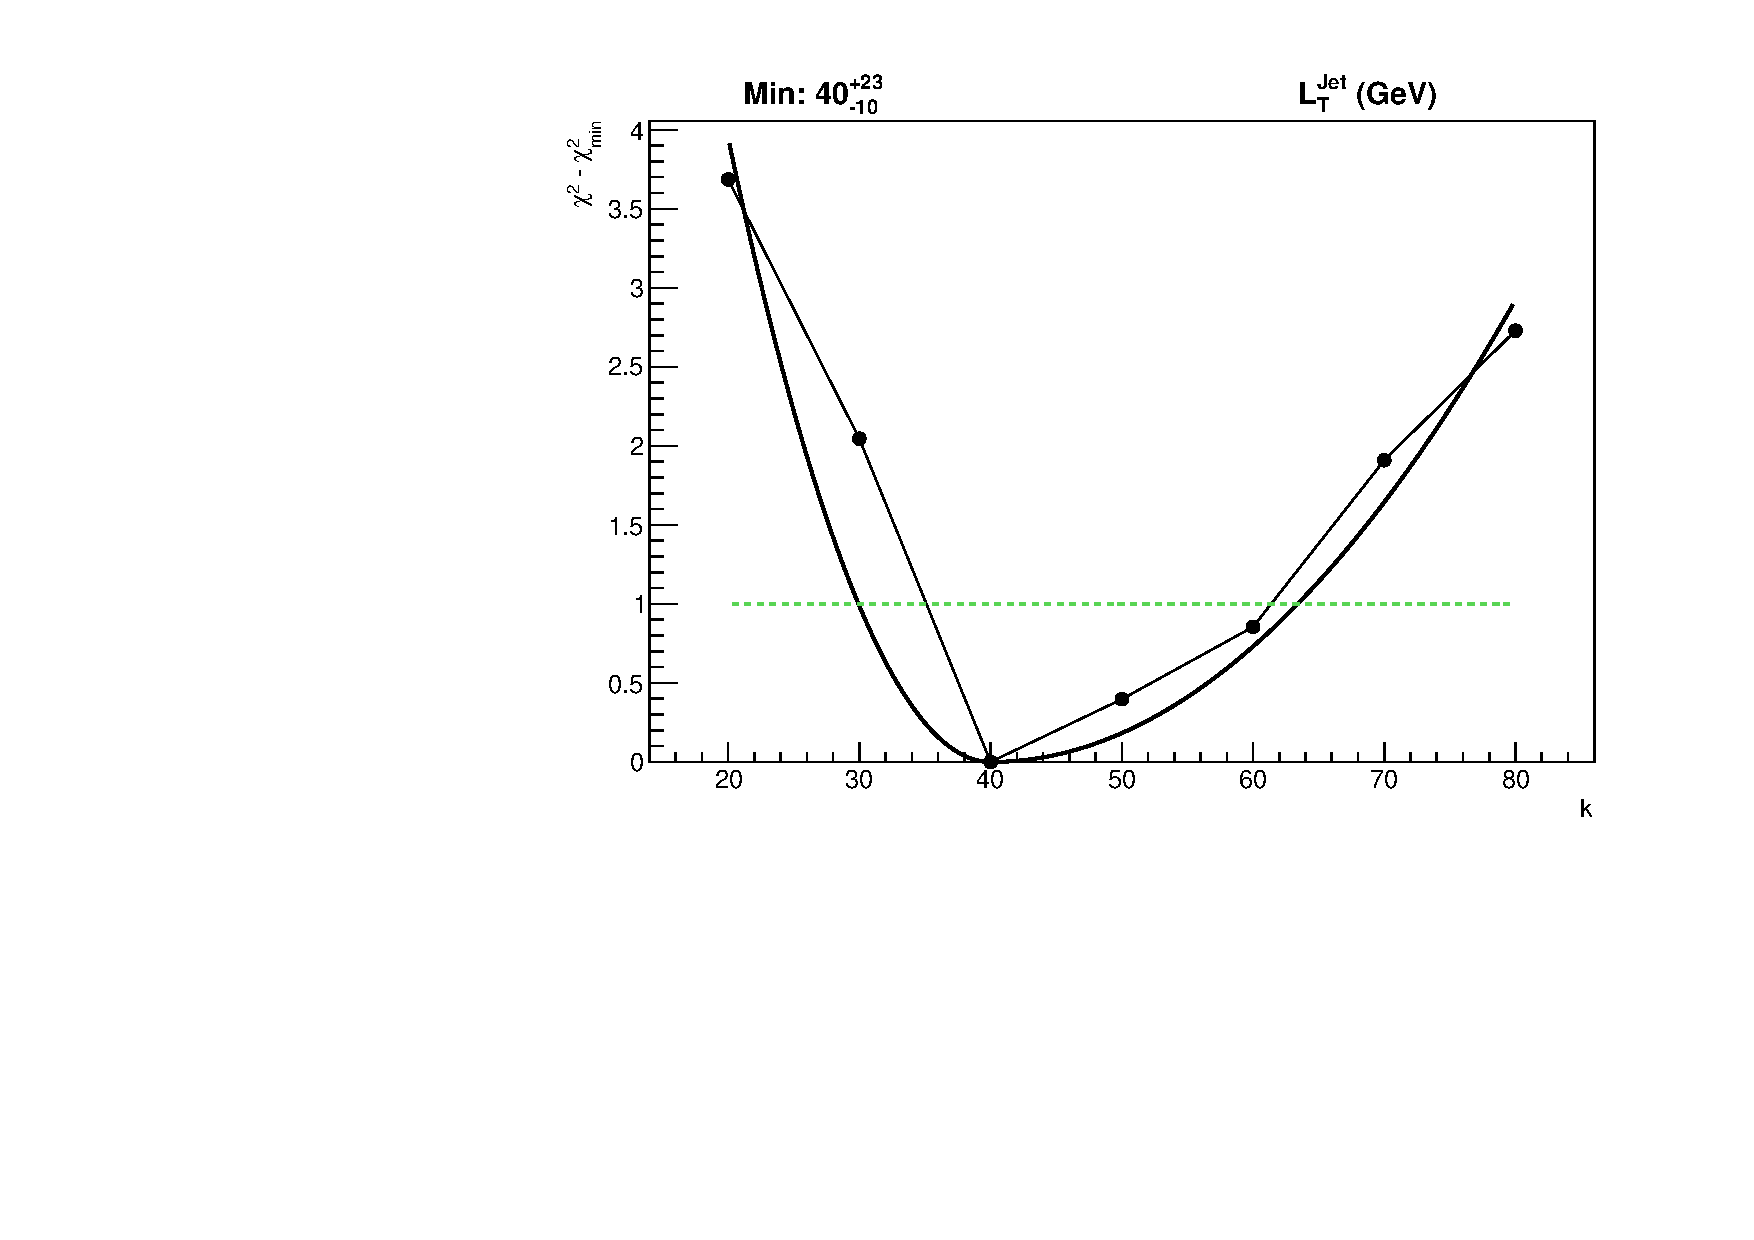
\includegraphics[width=0.5\textwidth]{4_Analisys/pics/8TeV/ProfileNeighbors/MM/h2taucuts020_LT.pdf} \\
\caption{\chisq scan of different neighbors value (left) and corresponding minima fit (right) for leading (top) and sub-leading (bottom) muons in $\mu\mu\tau_h$ channel. The variable used for the scan is the scalar sum of the \pT of the two leptons and the jet}
\label{fig:kNN_minima_MMT}
\end{figure}

\begin{figure}
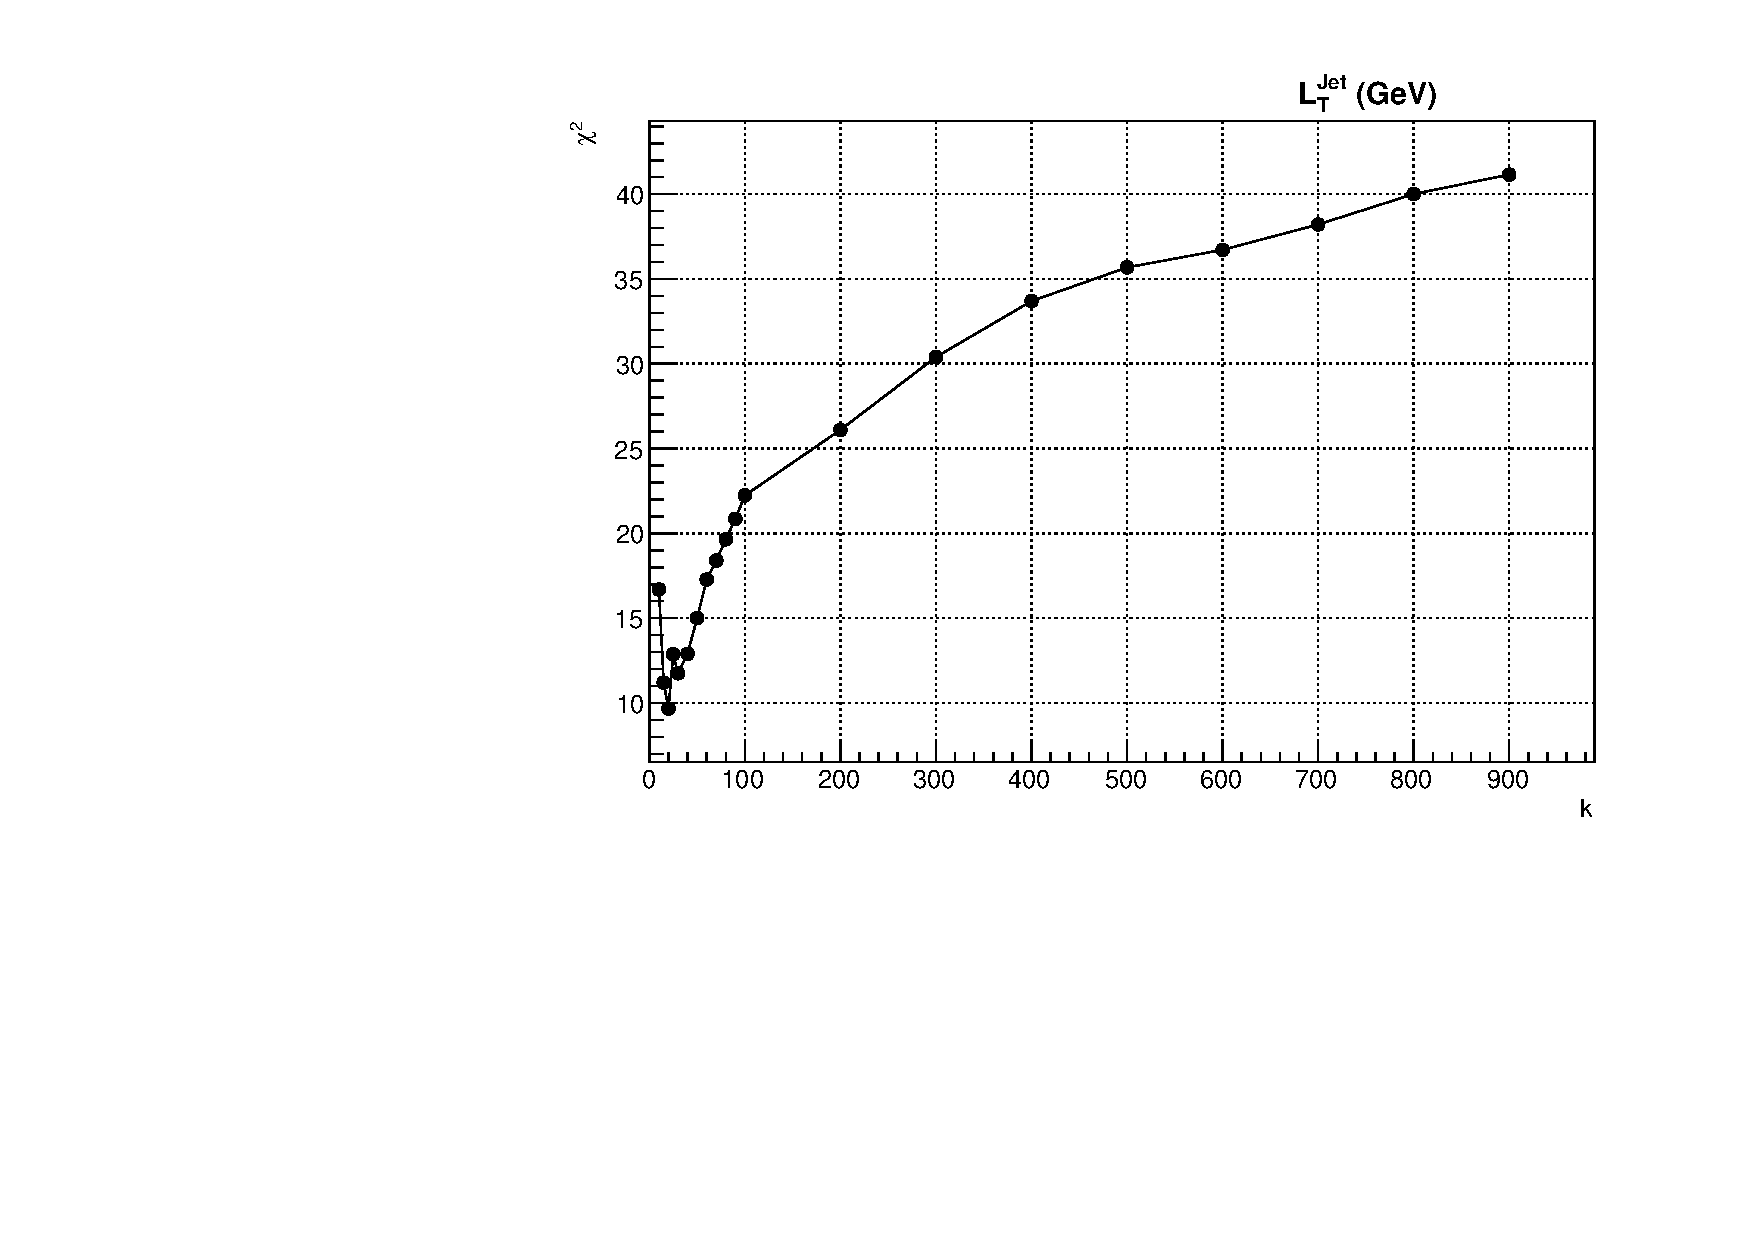
\includegraphics[width=0.5\textwidth]{4_Analisys/pics/8TeV/ProfileNeighbors/EM_Muon/h2taucuts/LT_chi2.pdf}
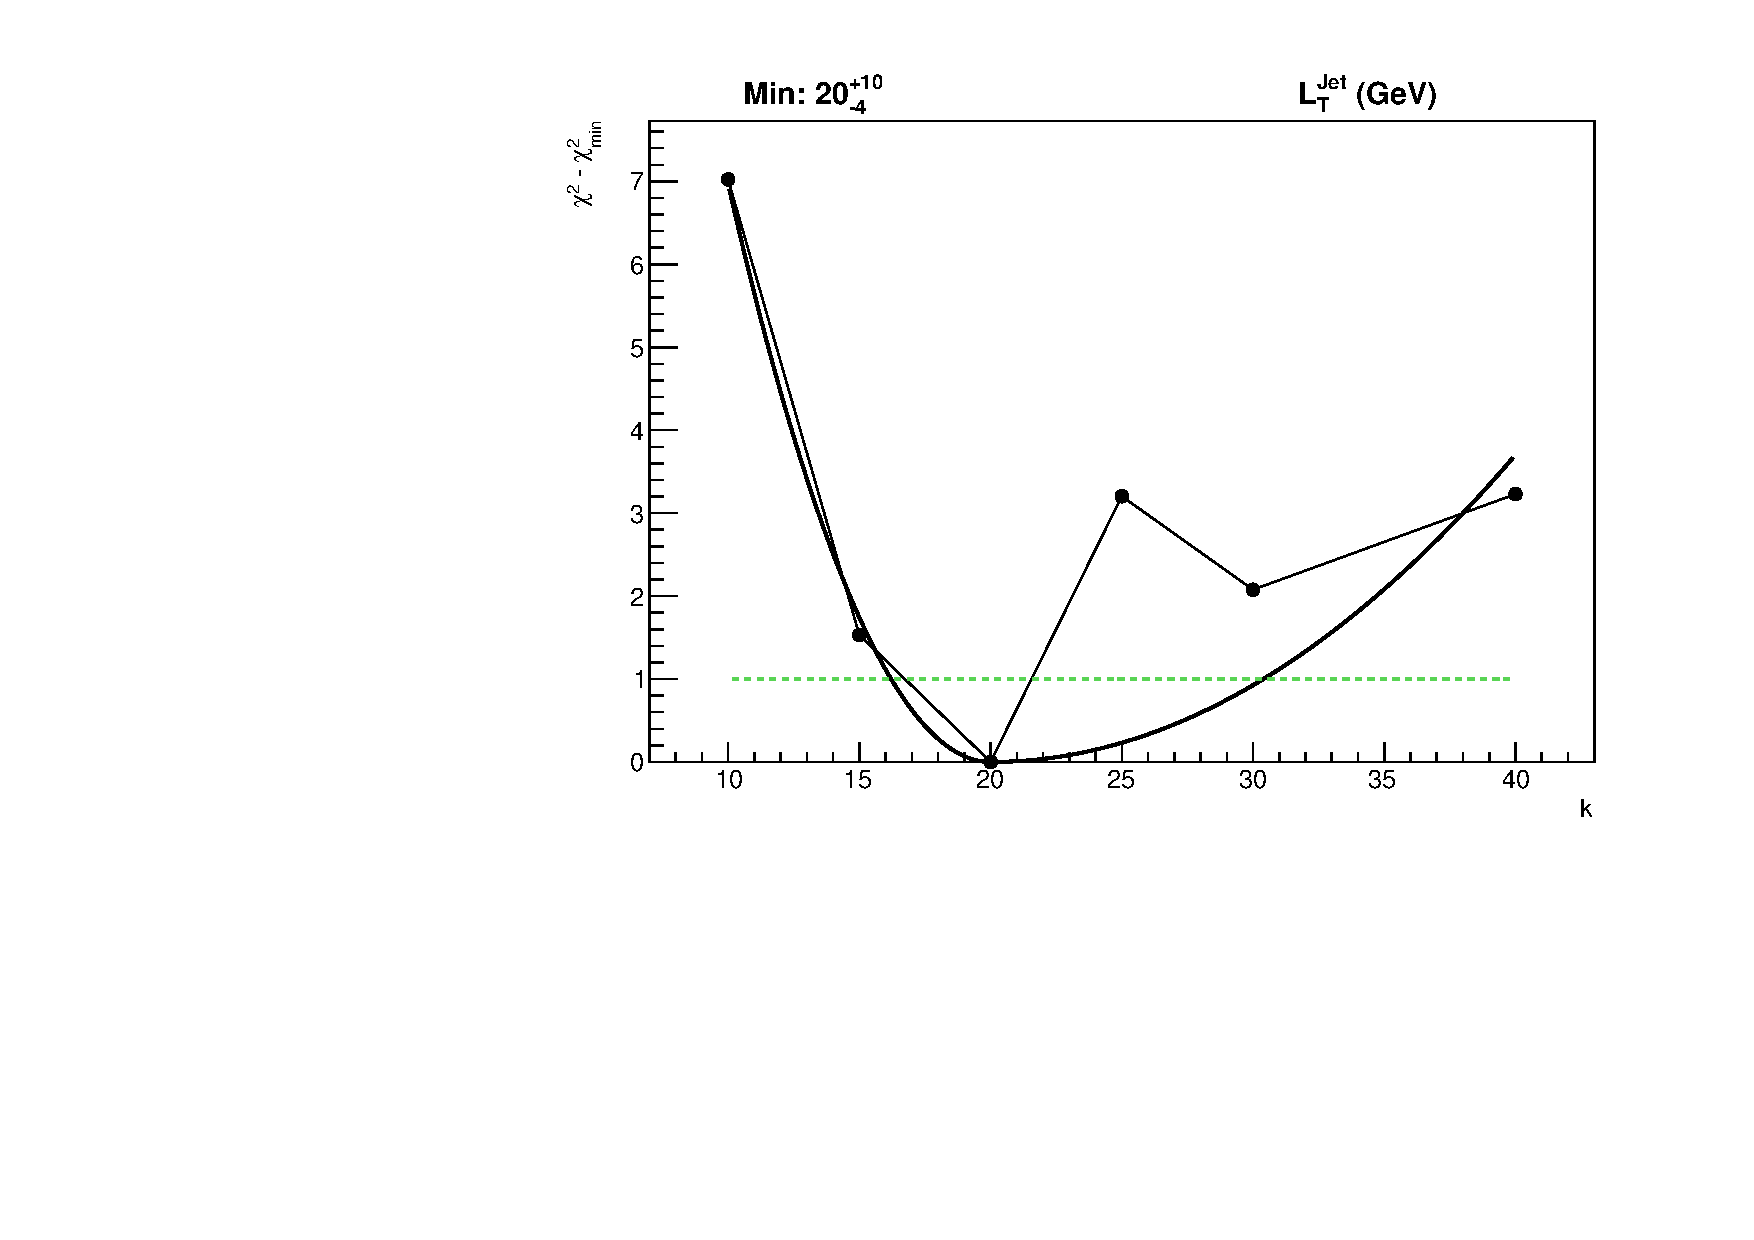
\includegraphics[width=0.5\textwidth]{4_Analisys/pics/8TeV/ProfileNeighbors/EM_Muon/h2taucuts_LT.pdf} \\
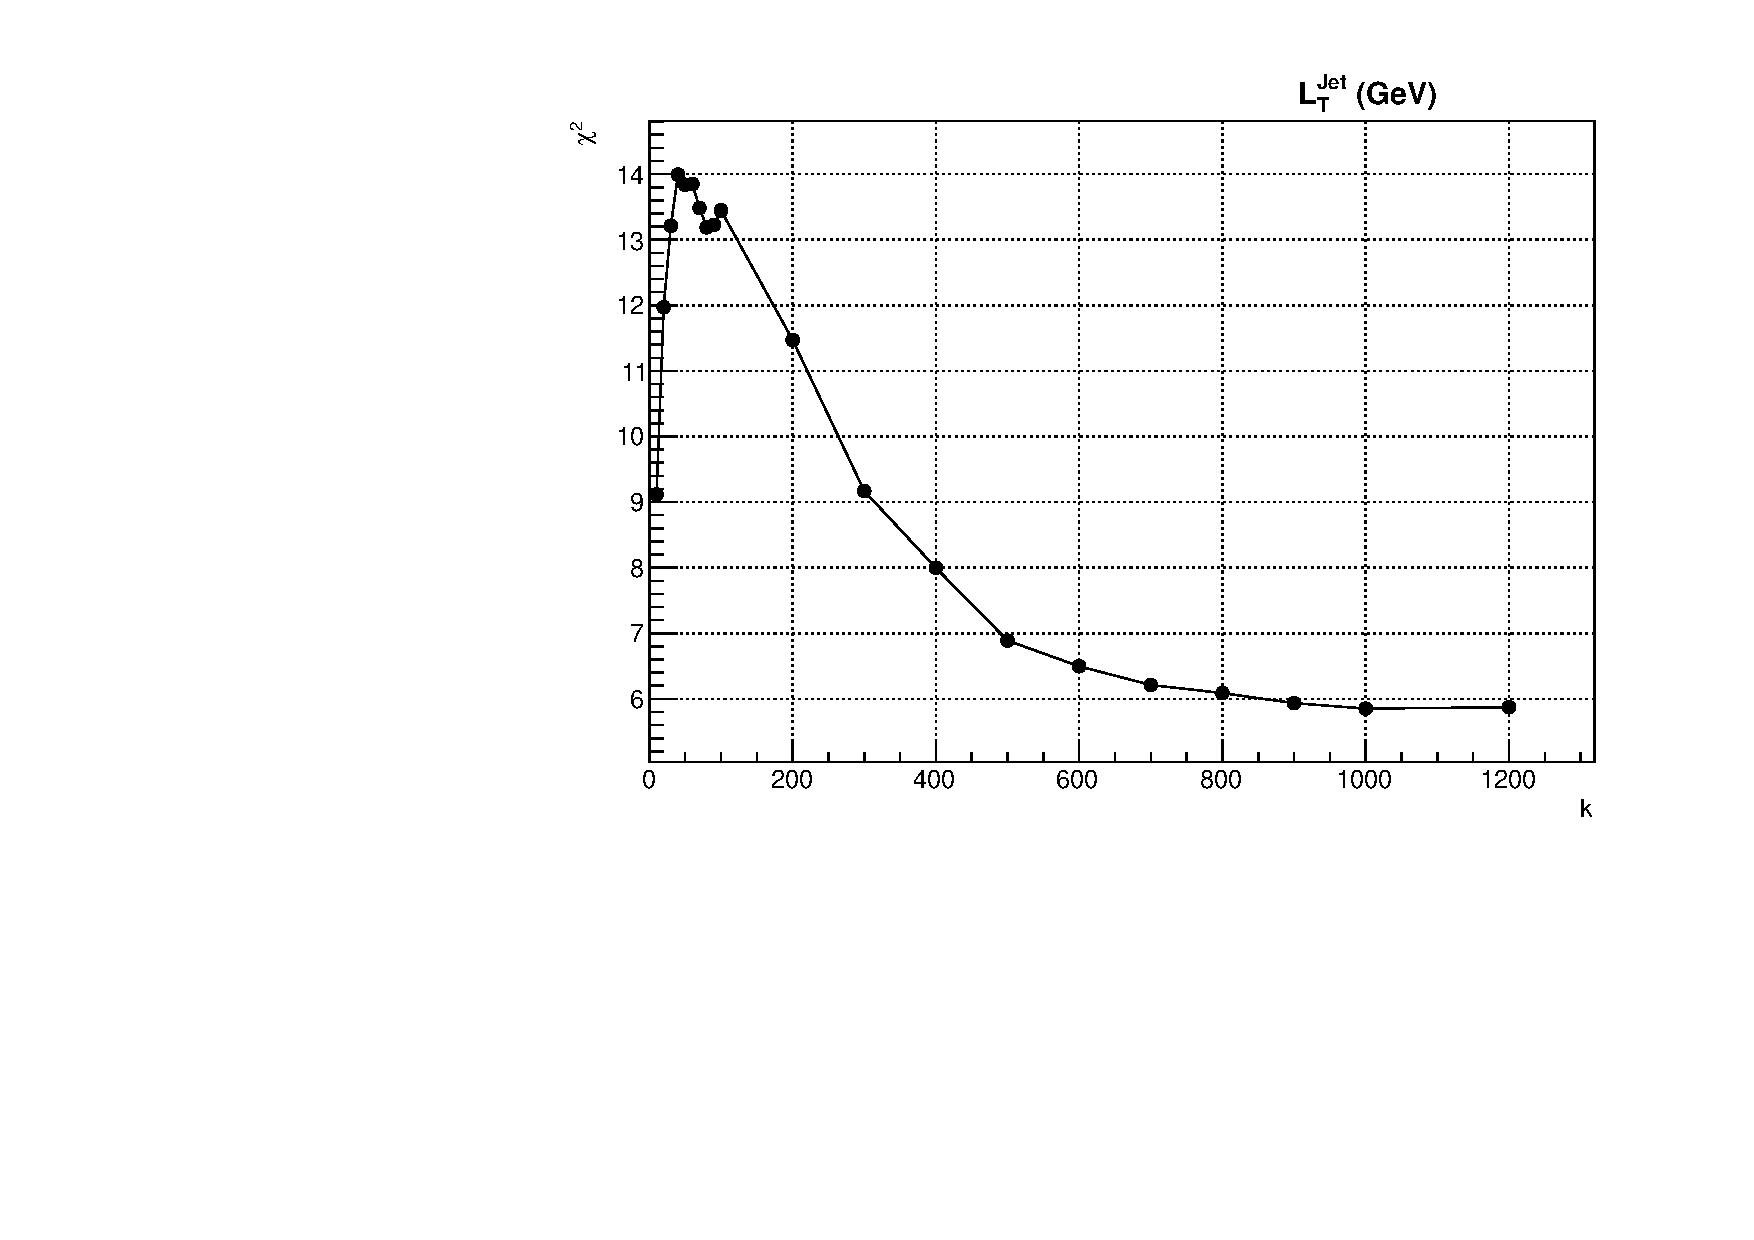
\includegraphics[width=0.5\textwidth]{4_Analisys/pics/8TeV/ProfileNeighbors/EM_Electron/eid12Medium_h2taucuts/LT_chi2.pdf}
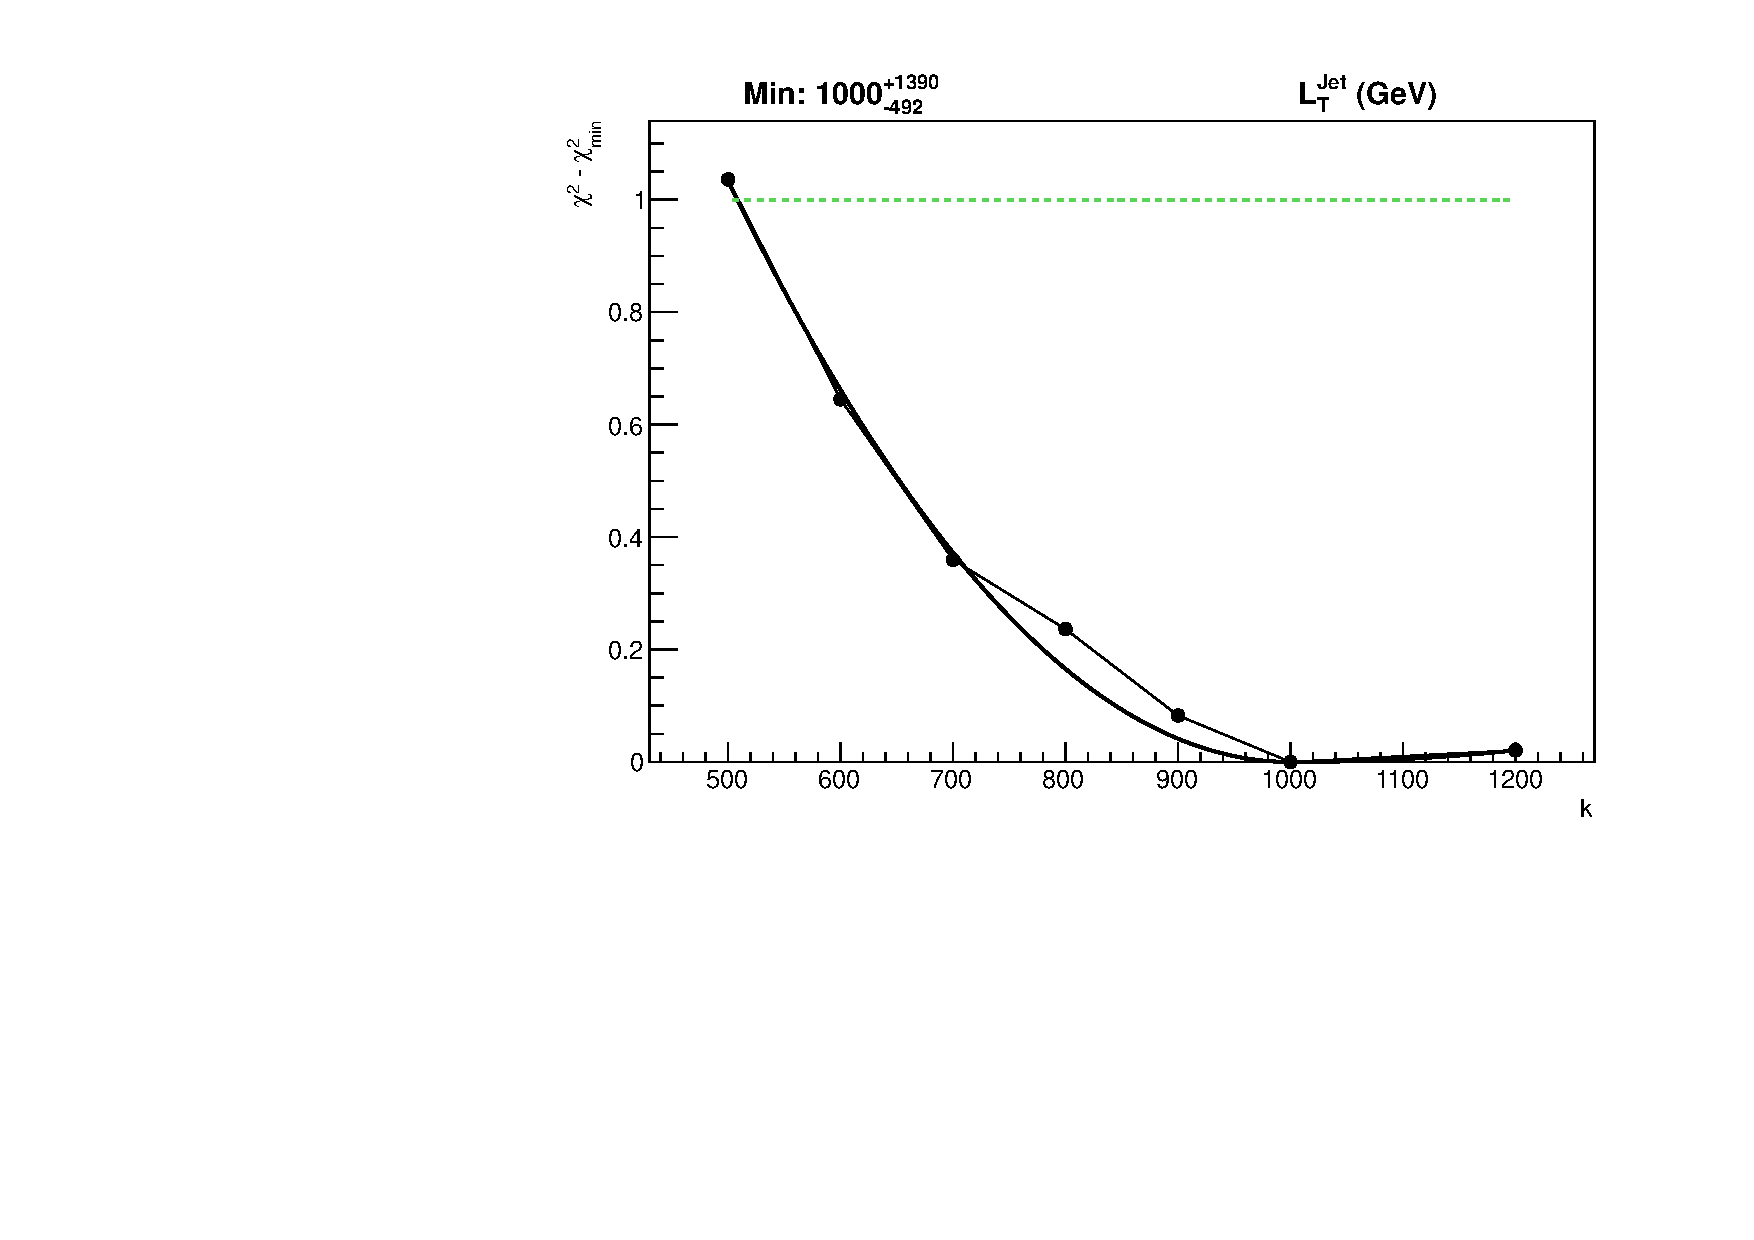
\includegraphics[width=0.5\textwidth]{4_Analisys/pics/8TeV/ProfileNeighbors/EM_Electron/eid12Medium_h2taucuts_LT.pdf} \\
\caption{\chisq scan of different neighbors value (left) and corresponding minima fit (right) for muon (top) and electron (bottom) in $e\mu\tau_h$ channel. The variable used for the scan is the scalar sum of the \pT of the two leptons and the jet}
\label{fig:kNN_minima_EMT}
\end{figure}

\begin{figure}
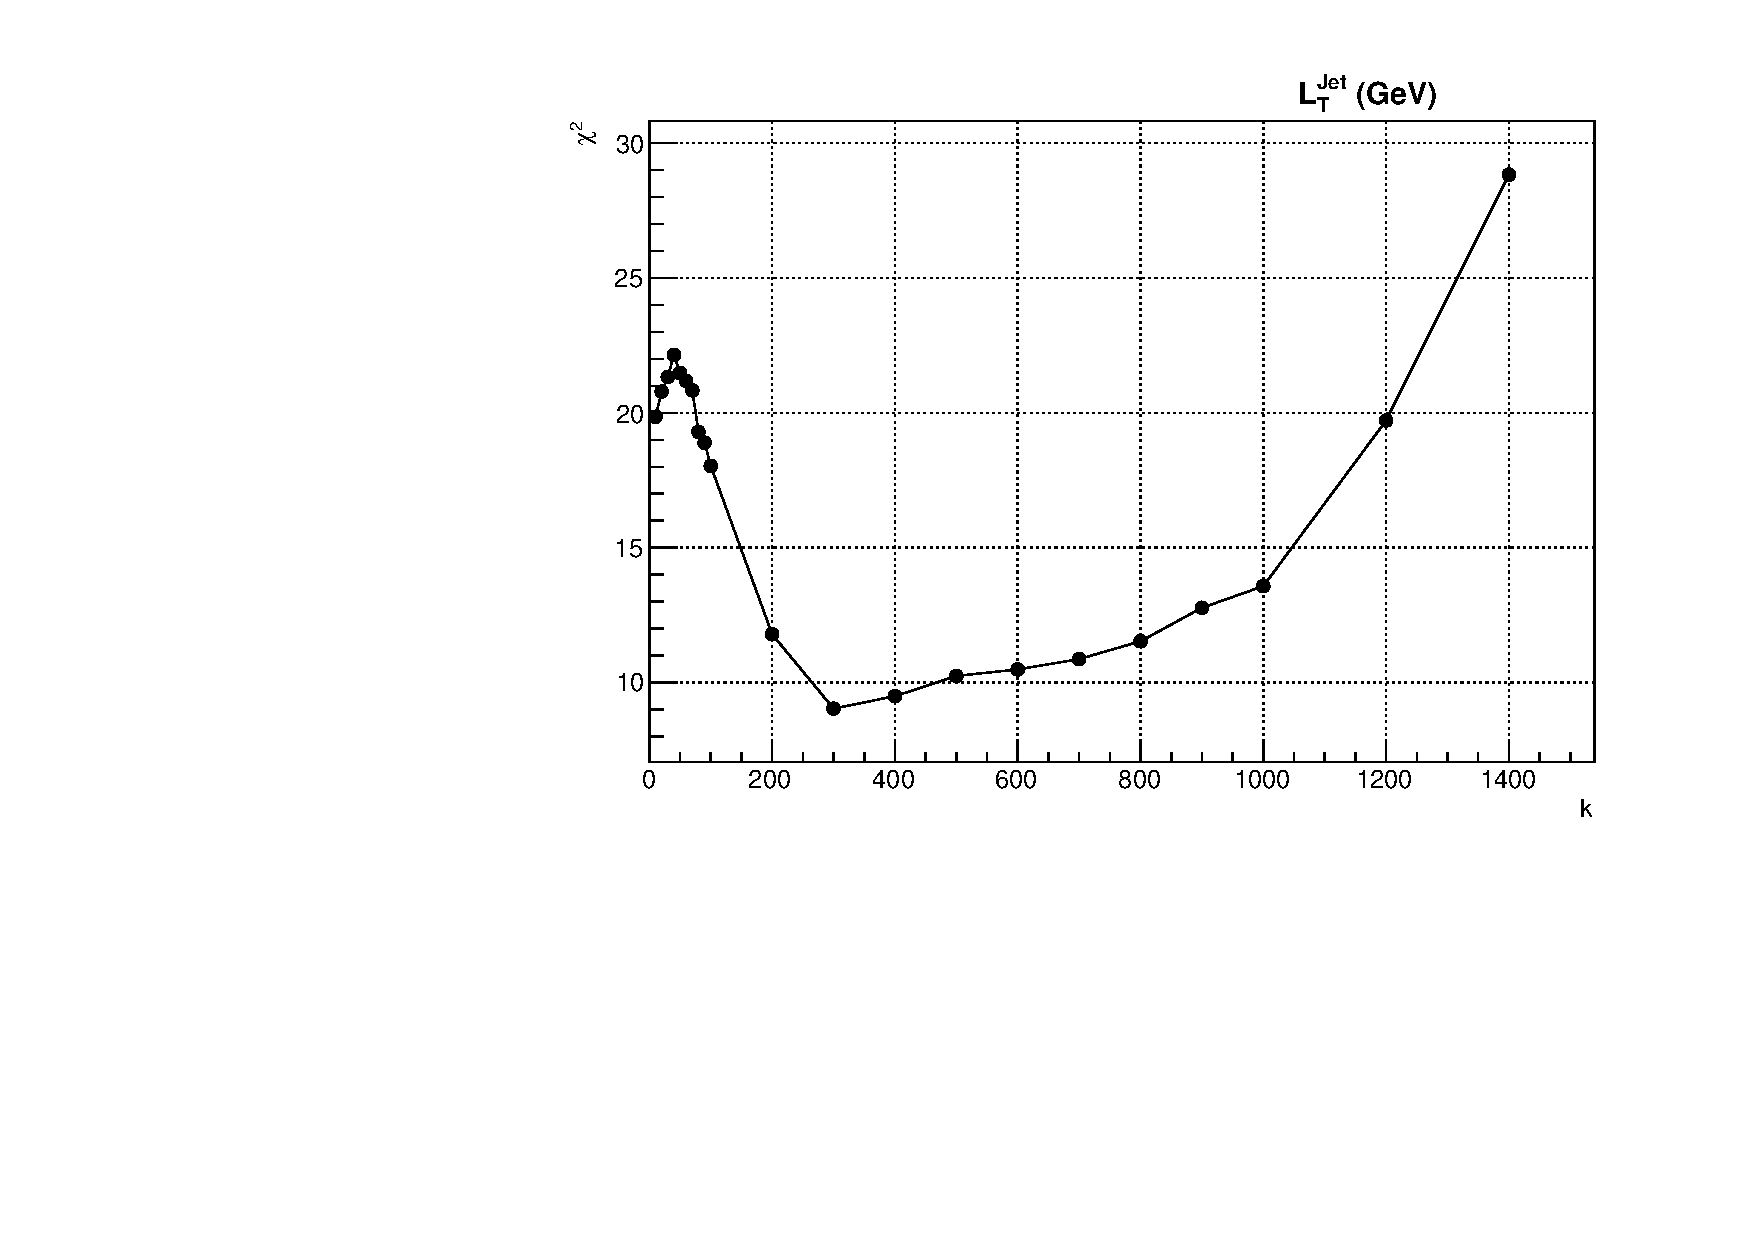
\includegraphics[width=0.5\textwidth]{4_Analisys/pics/8TeV/ProfileNeighbors/EE/eid12Tight_h2taucuts/LT_chi2.pdf}
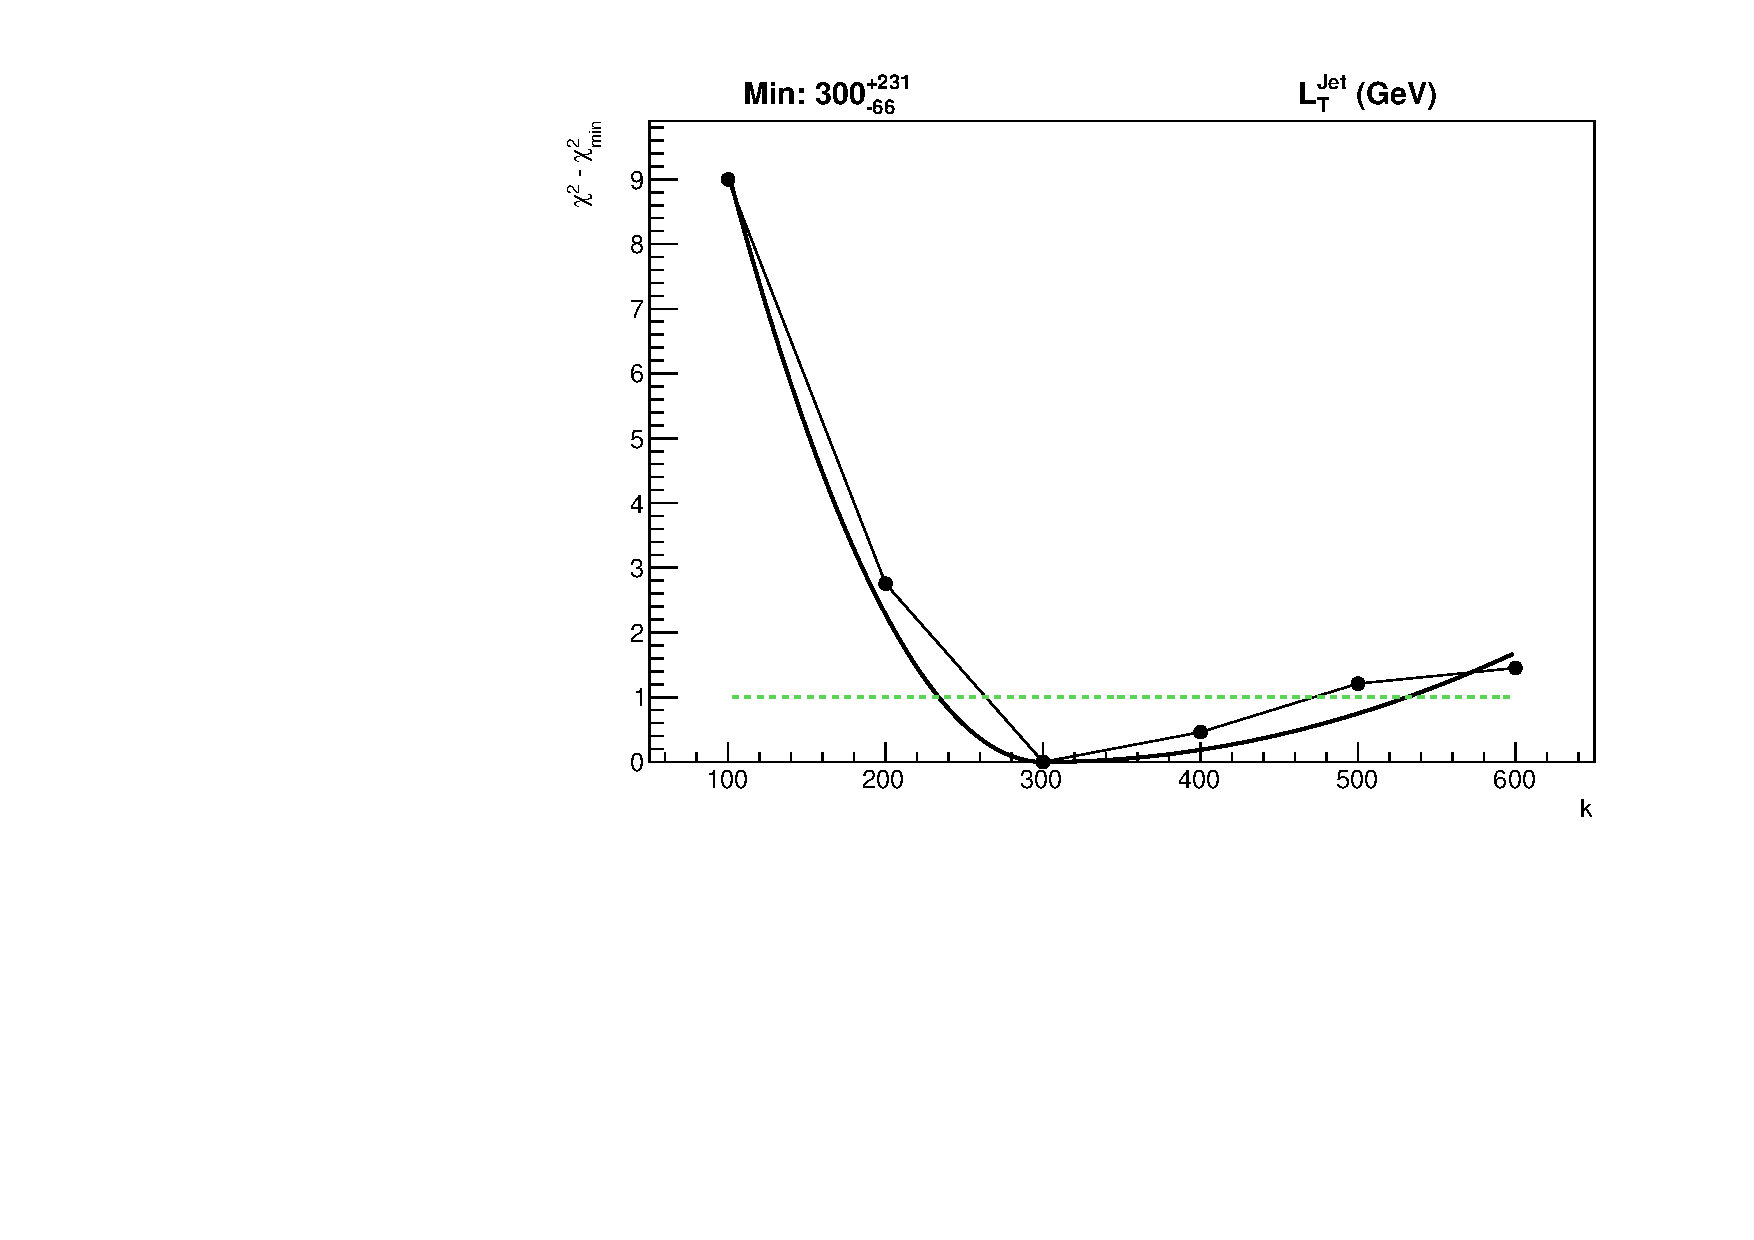
\includegraphics[width=0.5\textwidth]{4_Analisys/pics/8TeV/ProfileNeighbors/EE/eid12Tight_h2taucuts_LT.pdf} \\
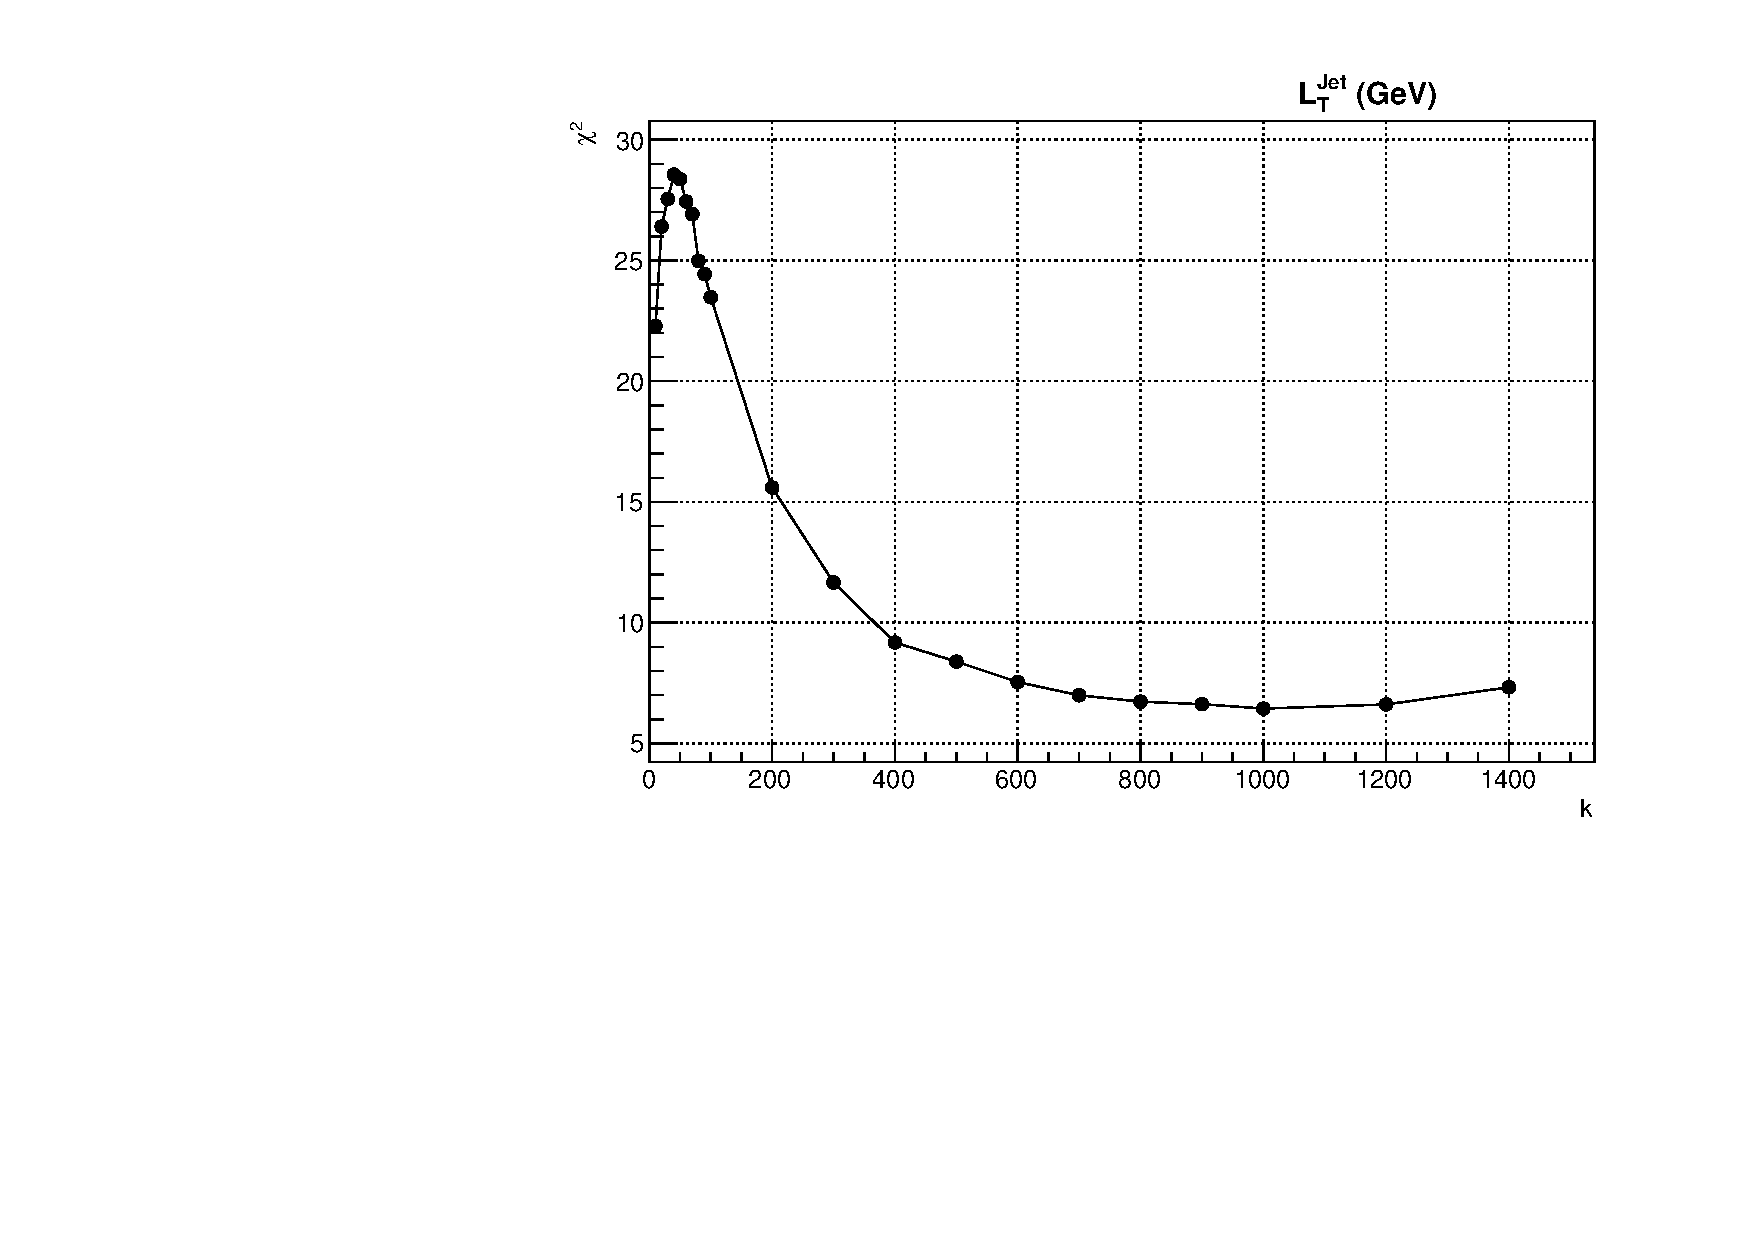
\includegraphics[width=0.5\textwidth]{4_Analisys/pics/8TeV/ProfileNeighbors/EE/eid12Medium_h2taucuts020/LT_chi2.pdf}
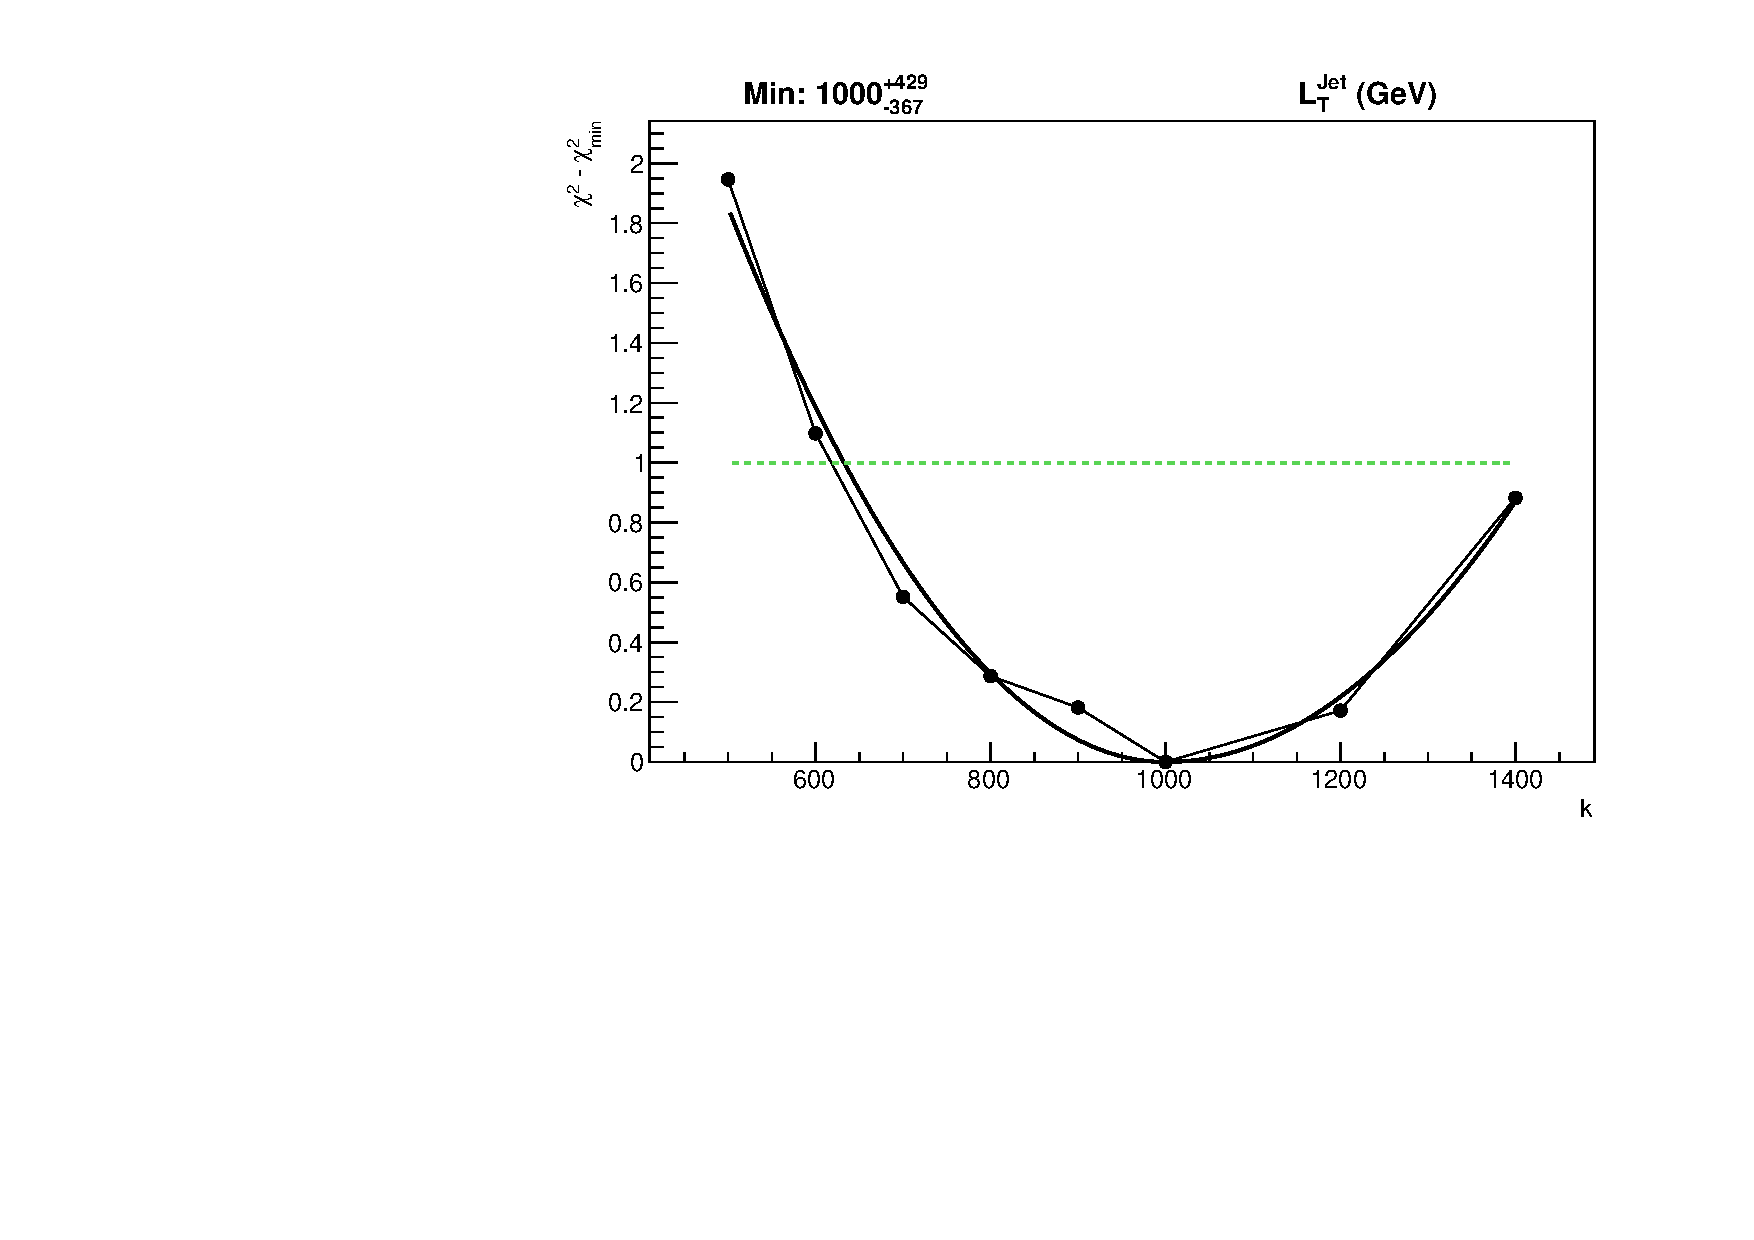
\includegraphics[width=0.5\textwidth]{4_Analisys/pics/8TeV/ProfileNeighbors/EE/eid12Medium_h2taucuts020_LT.pdf} \\
\caption{\chisq scan of different neighbors value (left) and corresponding minima fit (right) for leading (top) and sub-leading (bottom) electrons in $ee\tau_h$ channel. The variable used for the scan is the scalar sum of the \pT of the two leptons and the jet}
\label{fig:kNN_minima_EET}
\end{figure}

\begin{figure}
        \centering
        \begin{subfigure}[b]{0.33\textwidth}
		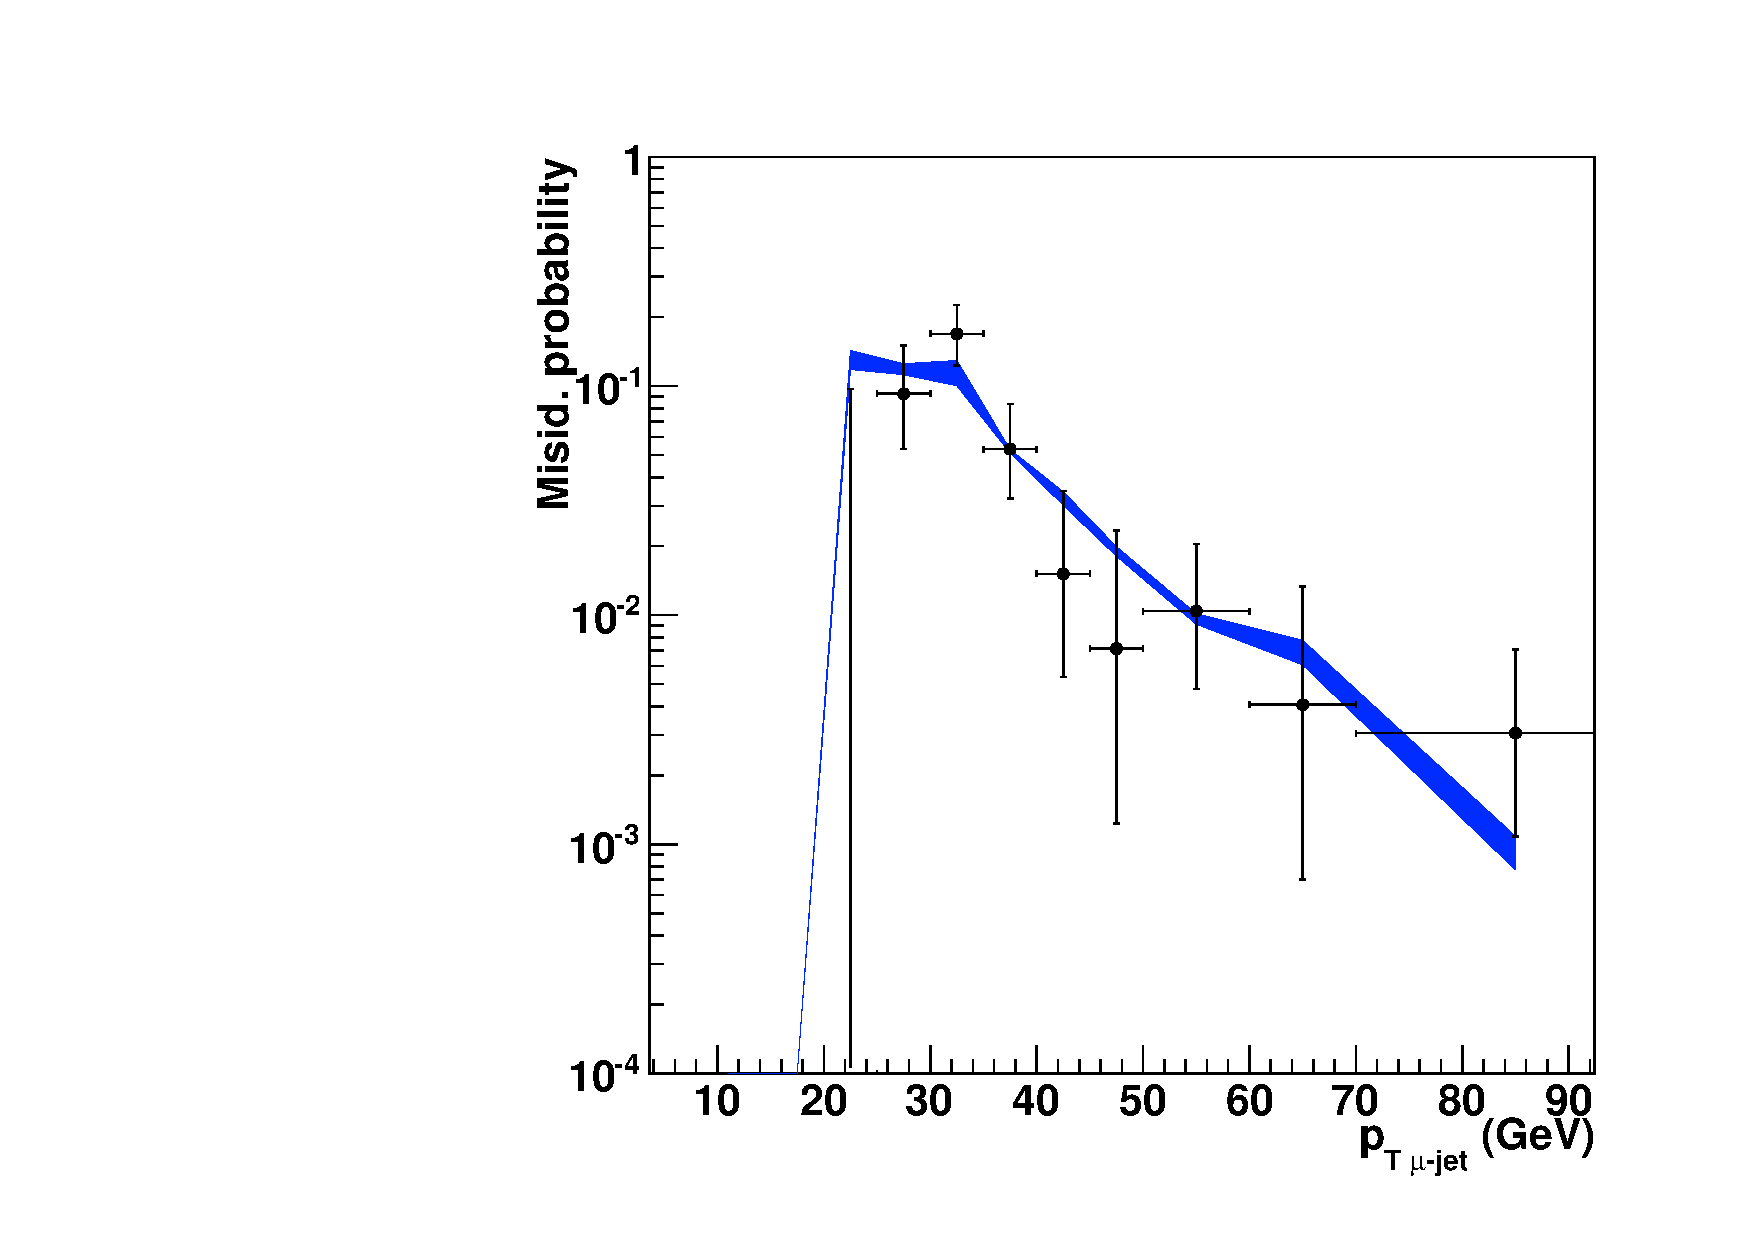
\includegraphics[width=\textwidth]{4_Analisys/pics/8TeV/plots/fakerates/m_mmt_leading_kNN_muonJetPt.pdf}
                \caption{}
        \end{subfigure}%
        \begin{subfigure}[b]{0.33\textwidth}
                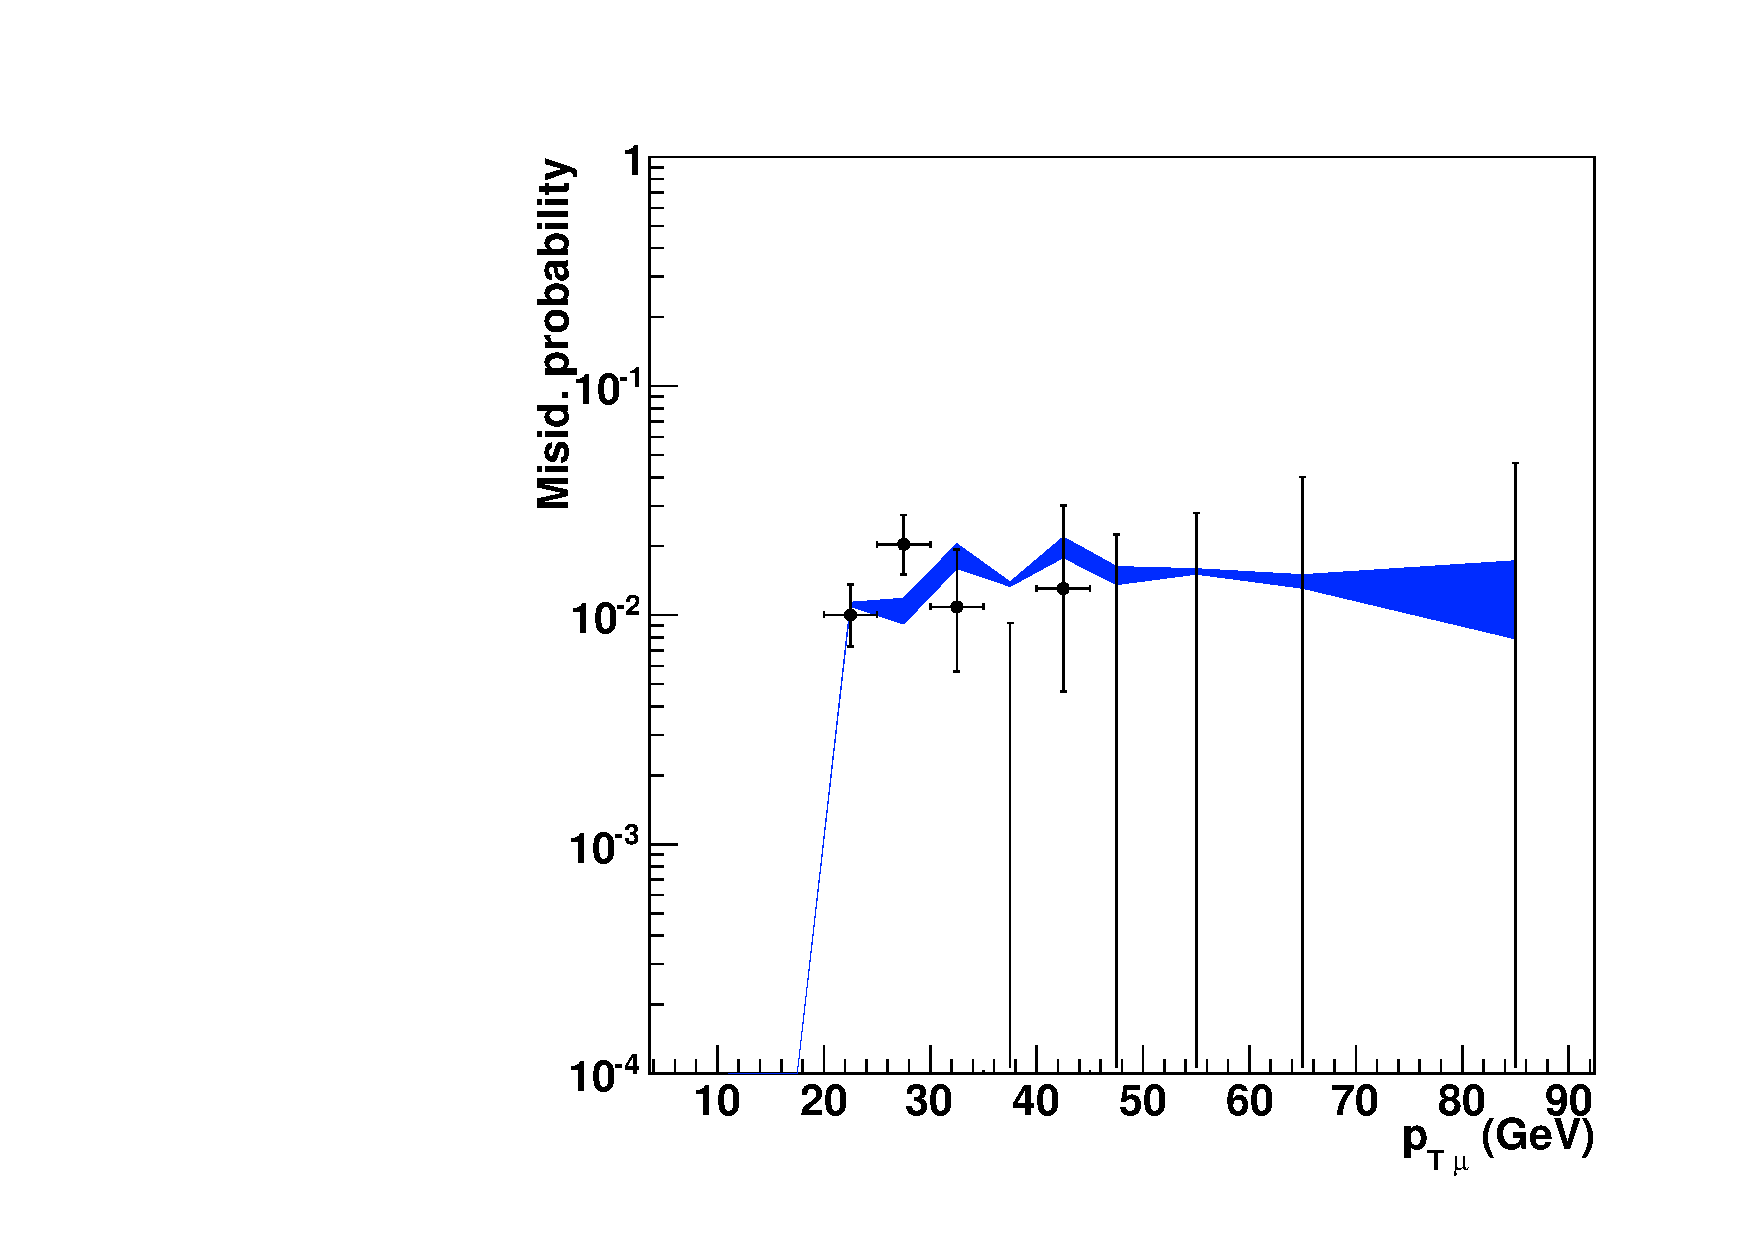
\includegraphics[width=\textwidth]{4_Analisys/pics/8TeV/plots/fakerates/m_mmt_leading_kNN_muonPt.pdf}
                \caption{}
        \end{subfigure}
        \begin{subfigure}[b]{0.33\textwidth}
                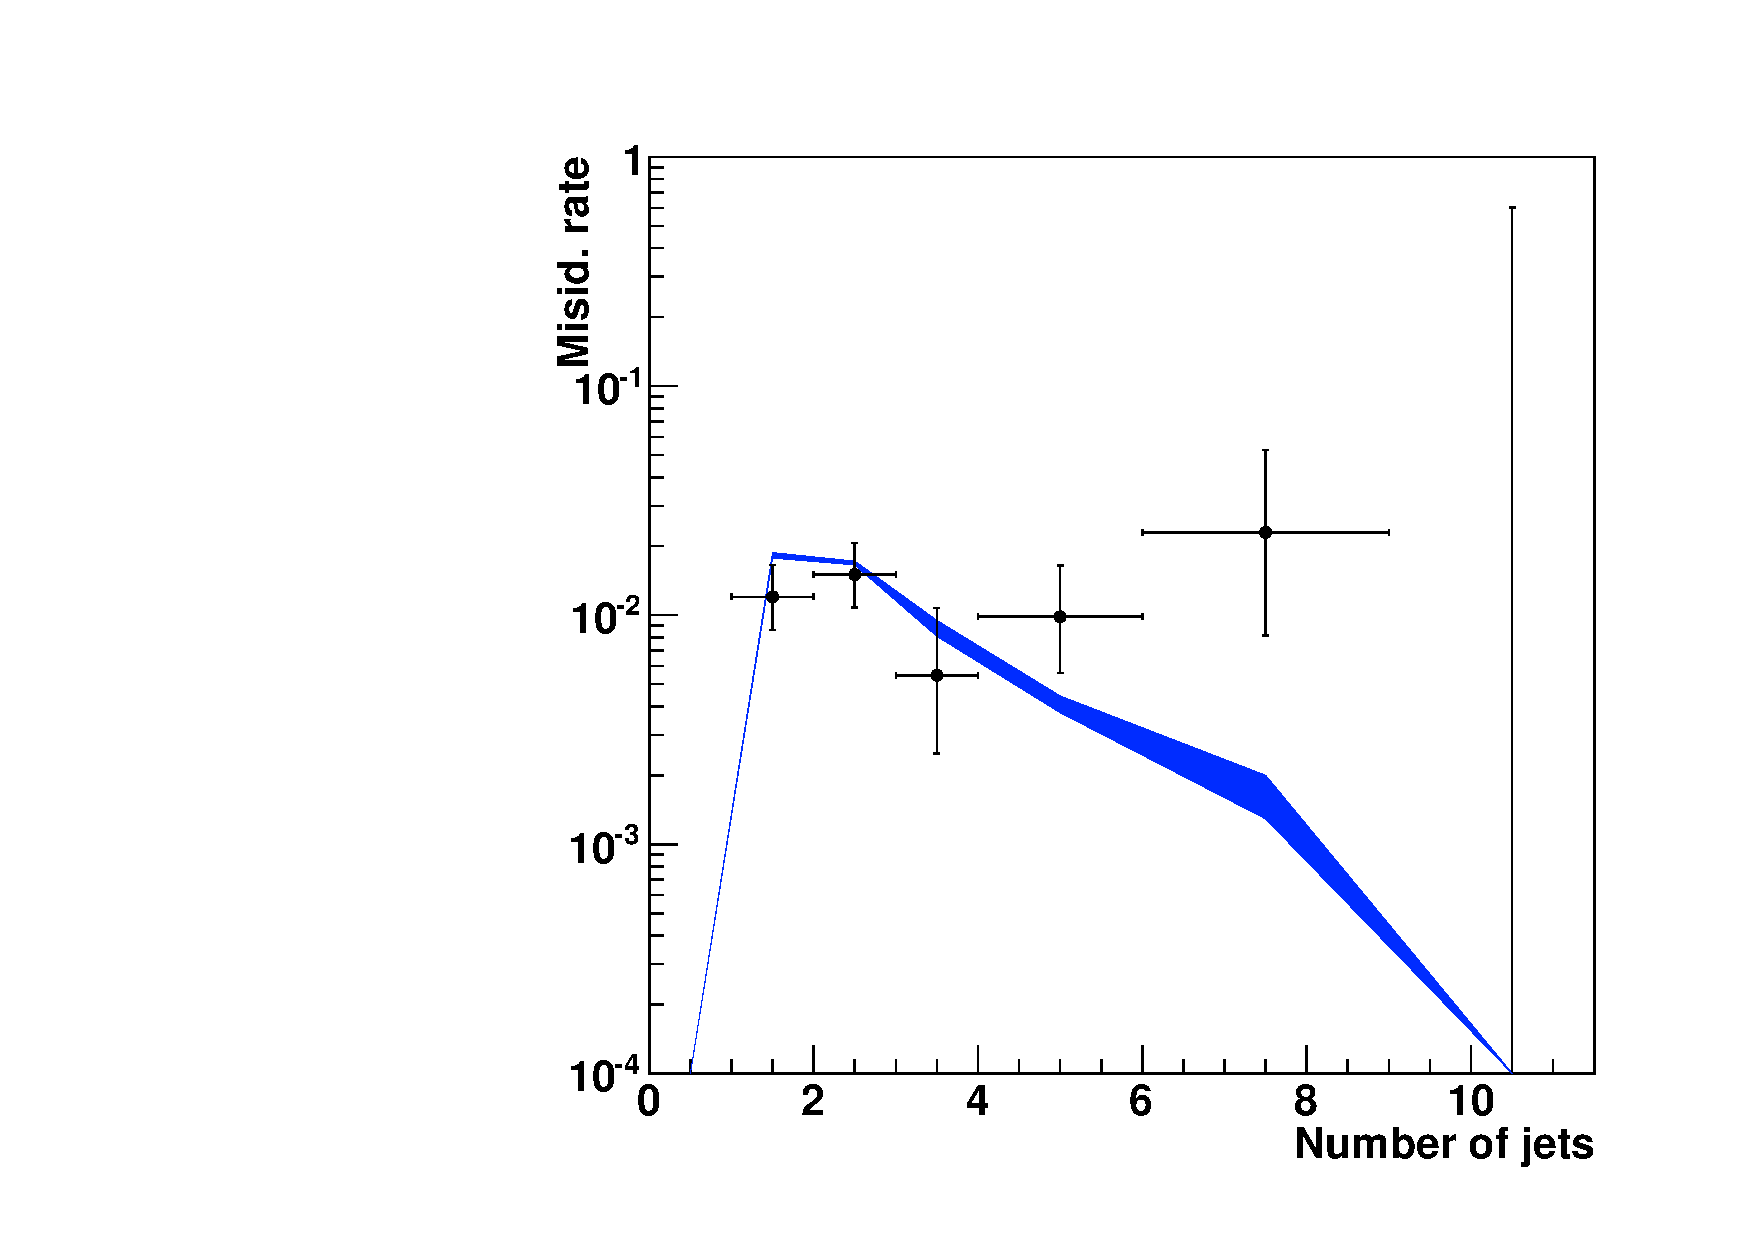
\includegraphics[width=\textwidth]{4_Analisys/pics/8TeV/plots/fakerates/m_mmt_leading_kNN_numJets20.pdf}
                \caption{}
        \end{subfigure}

        \begin{subfigure}[b]{0.33\textwidth}
		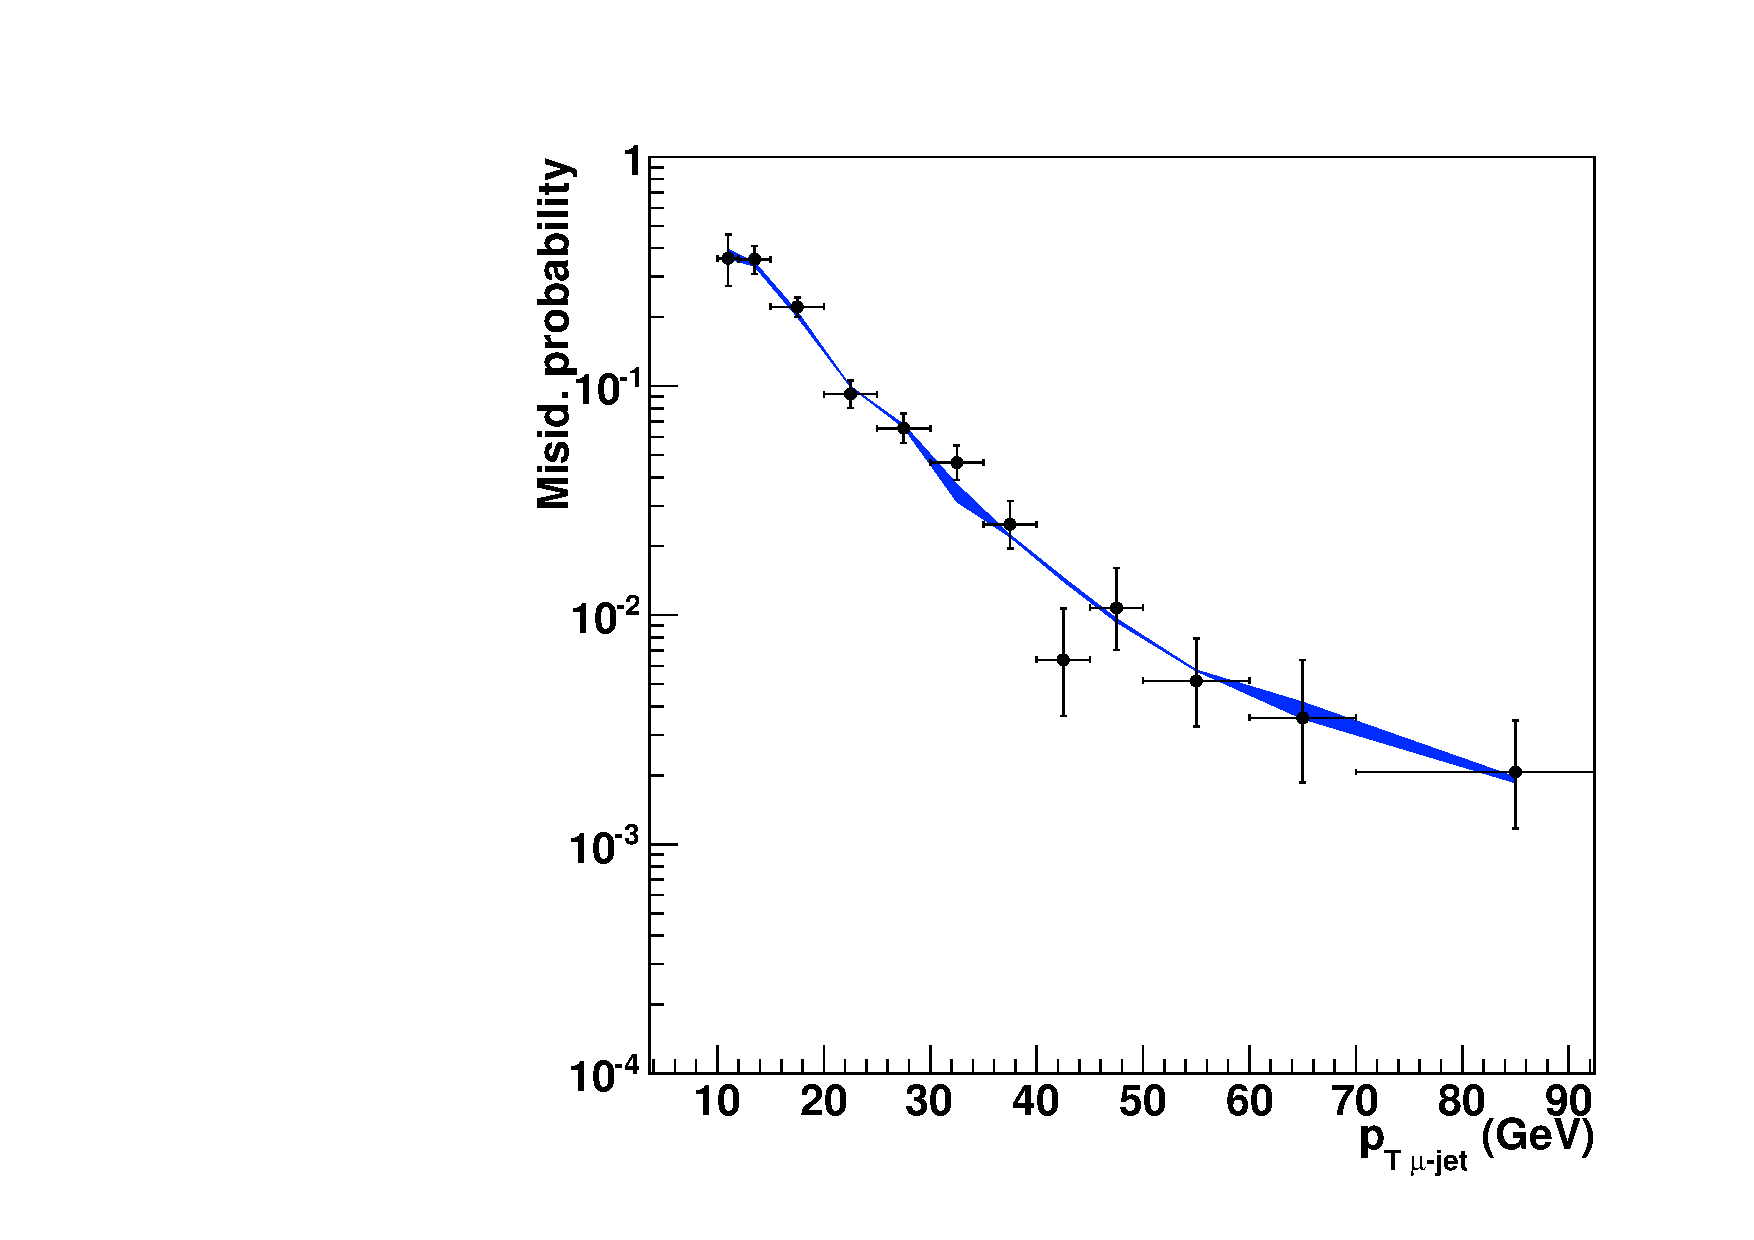
\includegraphics[width=\textwidth]{4_Analisys/pics/8TeV/plots/fakerates/m_mmt_subleading_kNN_muonJetPt.pdf}
                \caption{}
        \end{subfigure}%
        \begin{subfigure}[b]{0.33\textwidth}
                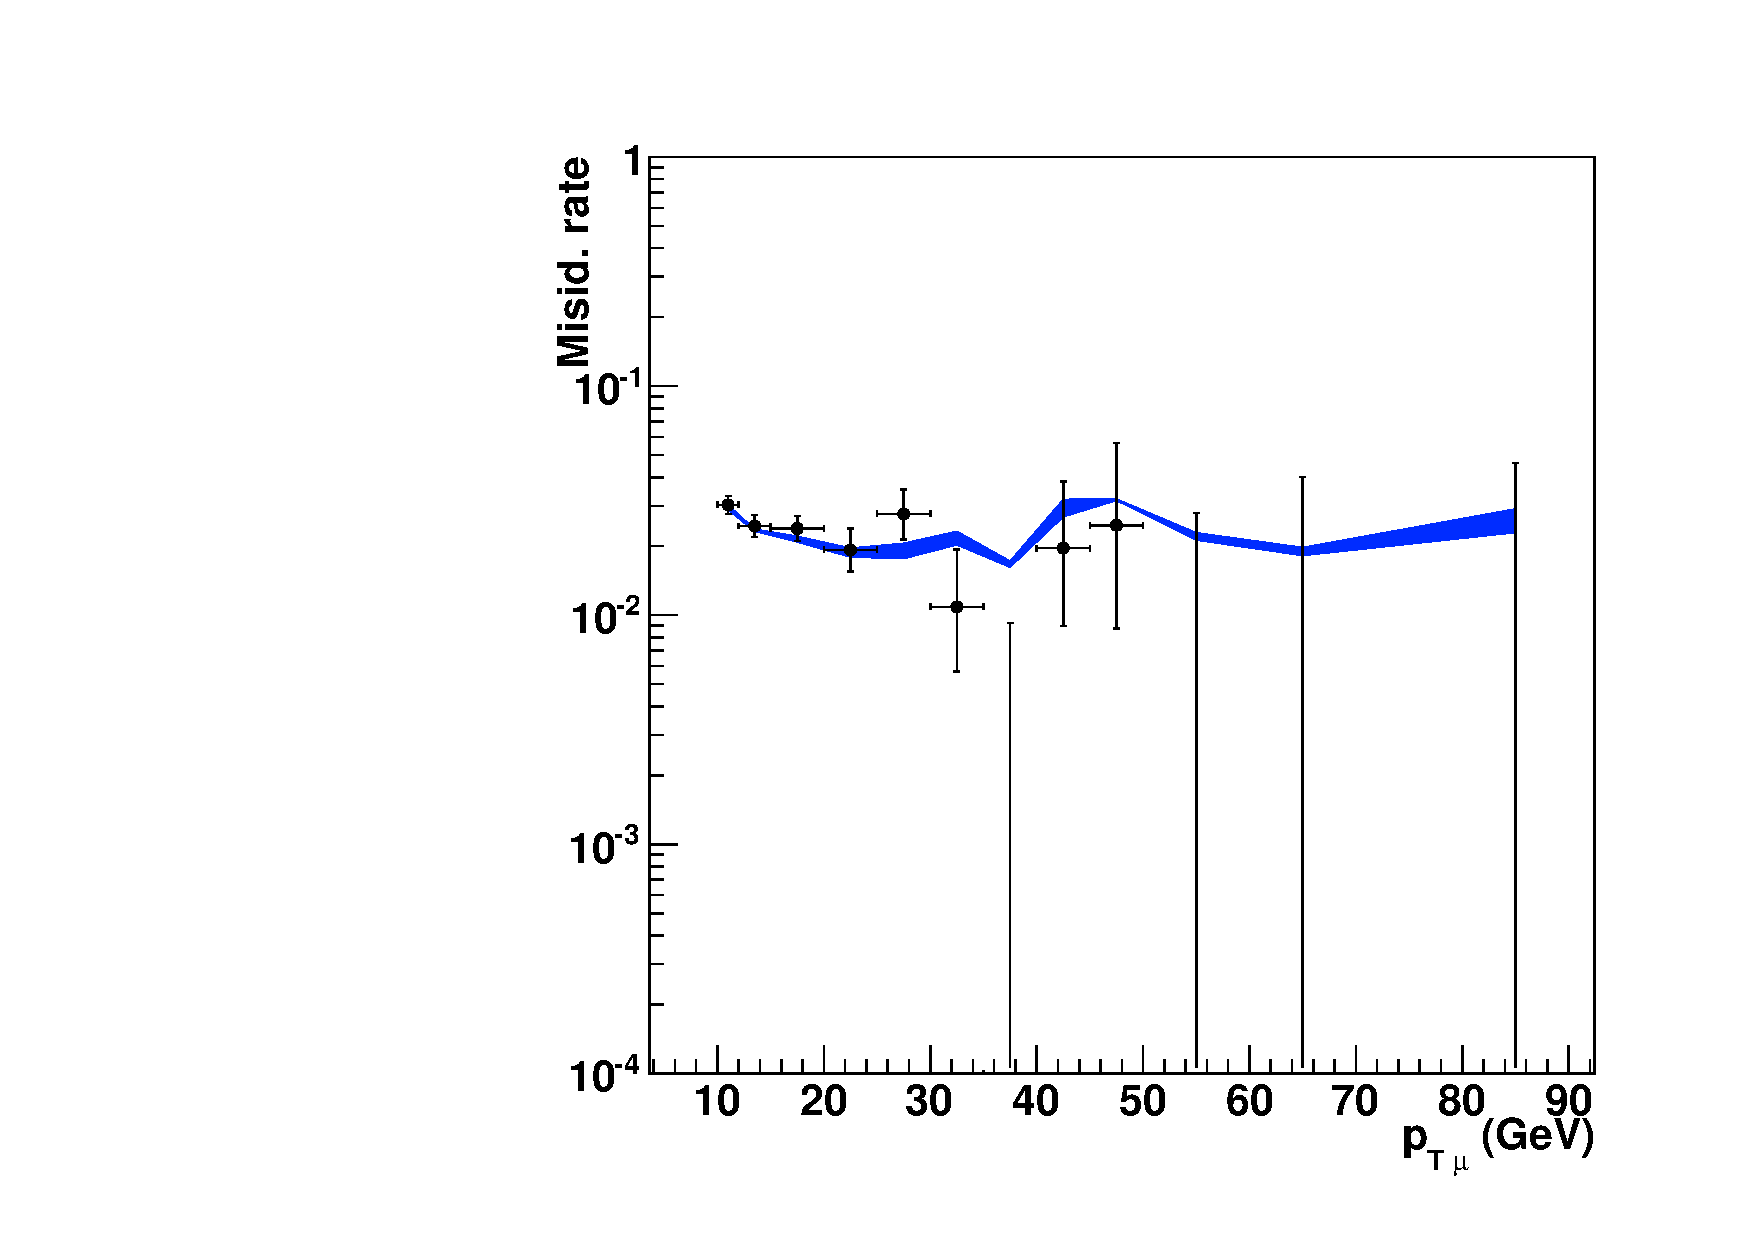
\includegraphics[width=\textwidth]{4_Analisys/pics/8TeV/plots/fakerates/m_mmt_subleading_kNN_muonPt.pdf}
                \caption{}
        \end{subfigure}
        \begin{subfigure}[b]{0.33\textwidth}
                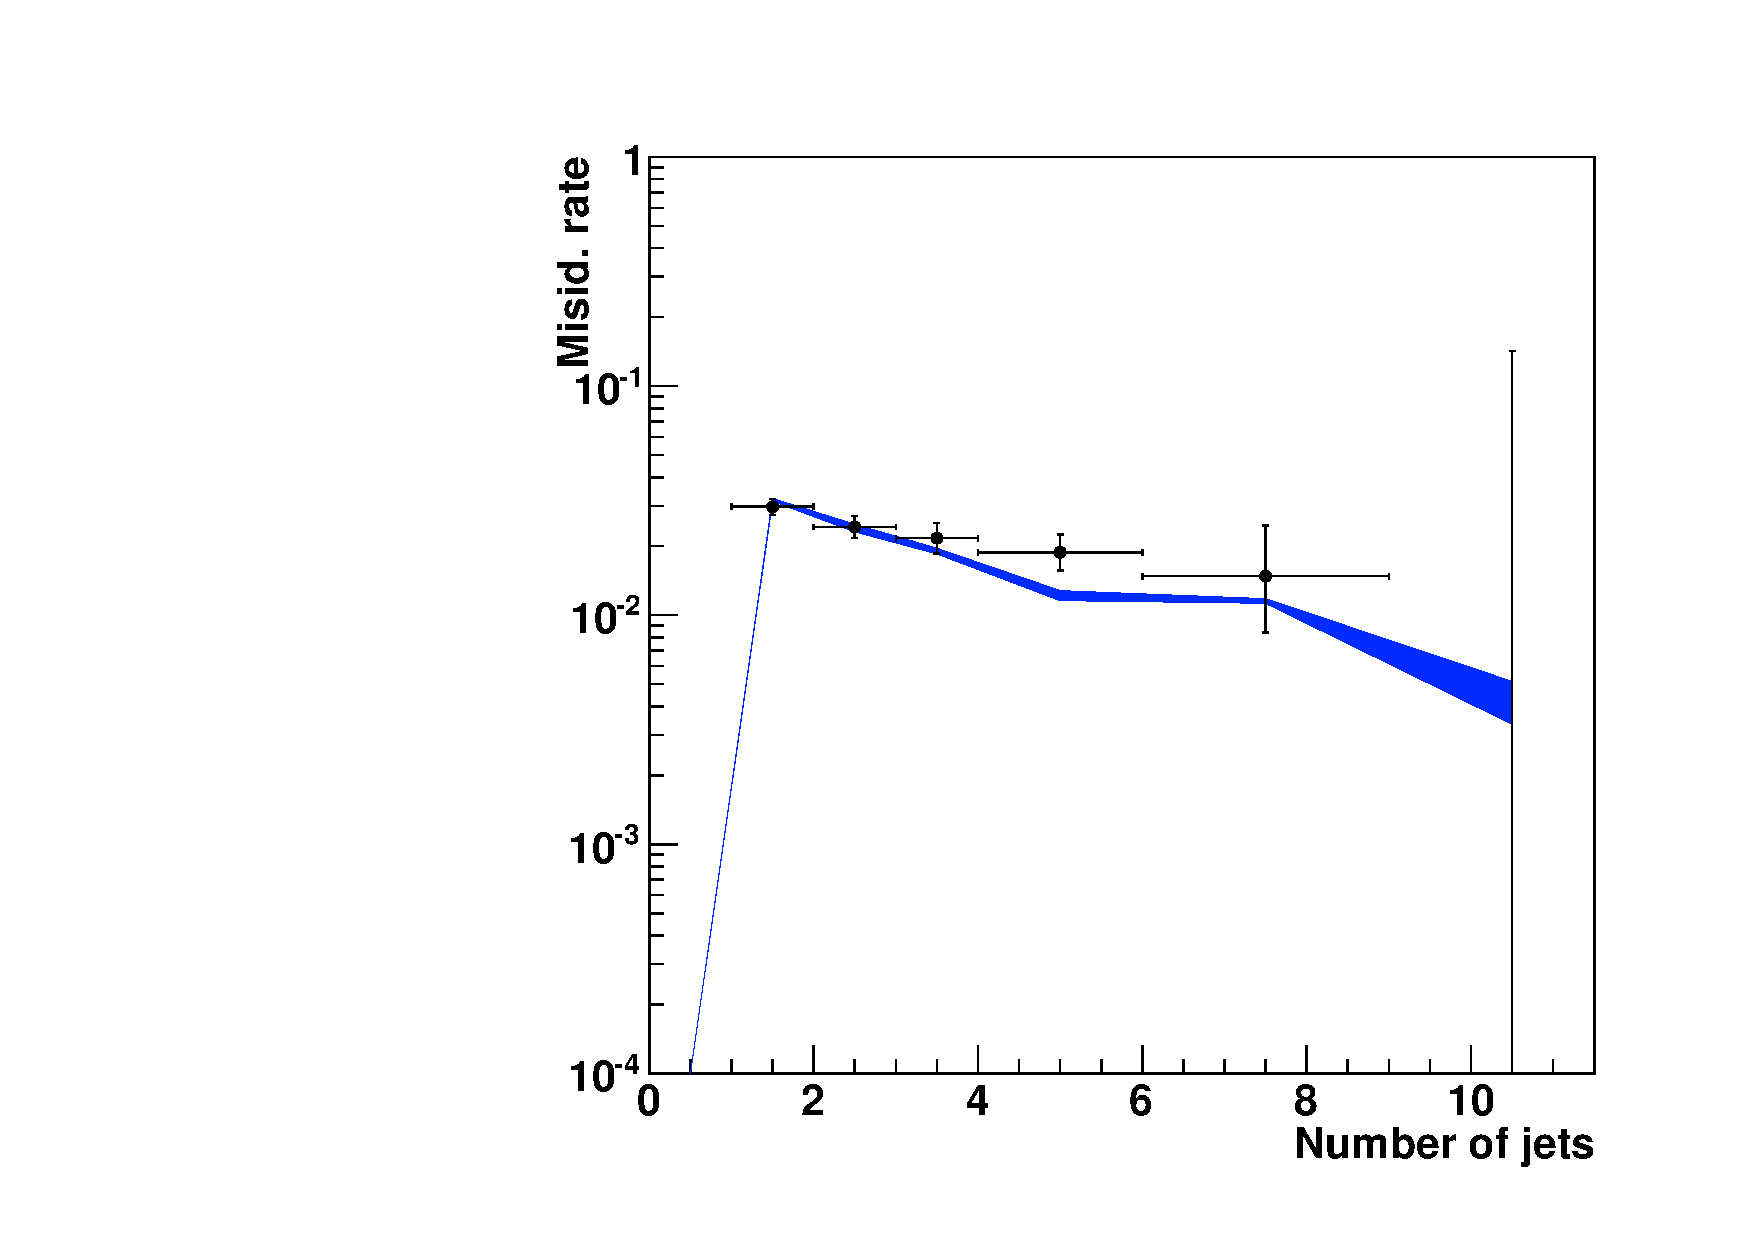
\includegraphics[width=\textwidth]{4_Analisys/pics/8TeV/plots/fakerates/m_mmt_subleading_kNN_numJets20.pdf}
                \caption{}
        \end{subfigure}
        \caption{Measured misidentification probability for leading (top) and sub-leading (bottom) muons in the training sample dedicated to the $\mu\mu\tau_h$ channel. The blue band represents the output of the kNN algorithm and its related uncertainty.}\label{fig:fake_rate_mmt}
\end{figure}

\begin{figure}
        \centering
        \begin{subfigure}[b]{0.33\textwidth}
		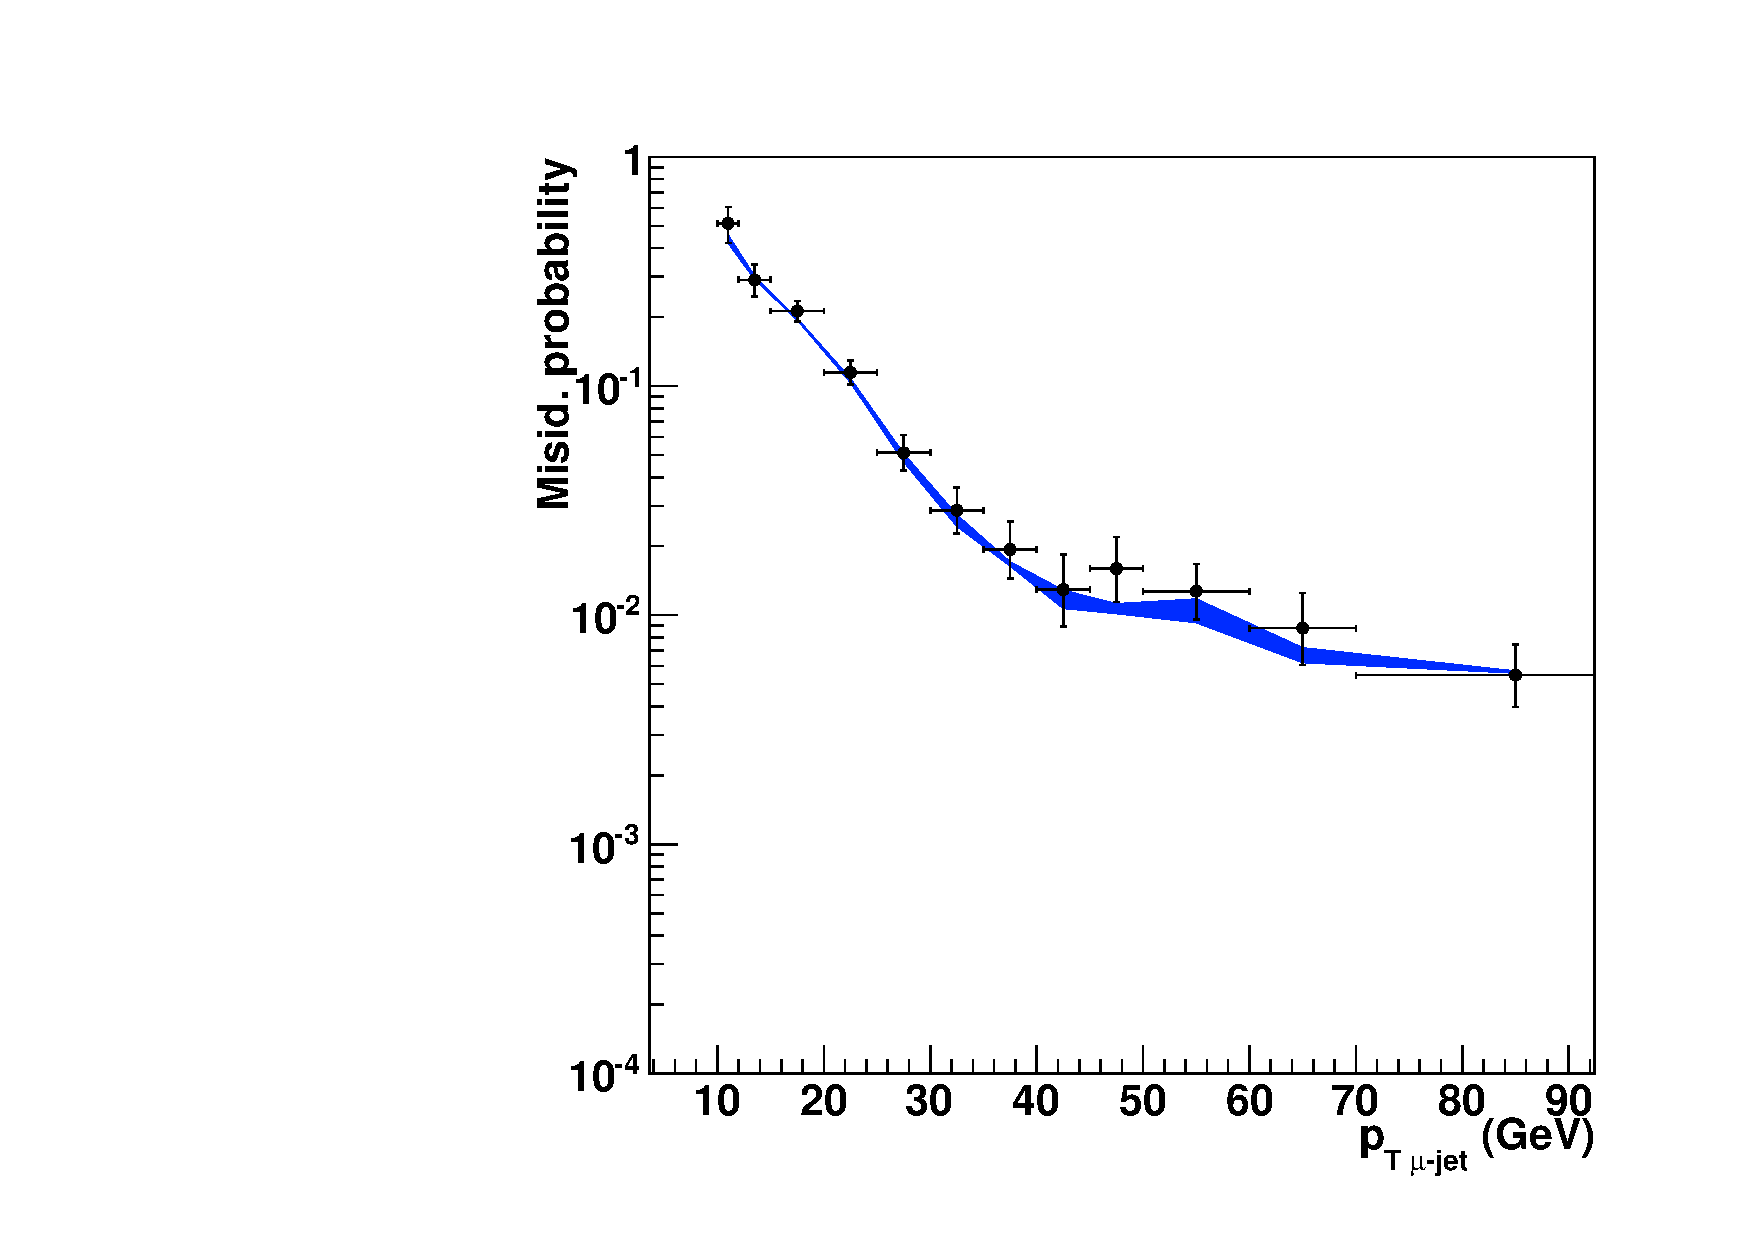
\includegraphics[width=\textwidth]{4_Analisys/pics/8TeV/plots/fakerates/m_emt_kNN_muonJetPt.pdf}
                \caption{}
        \end{subfigure}%
        \begin{subfigure}[b]{0.33\textwidth}
                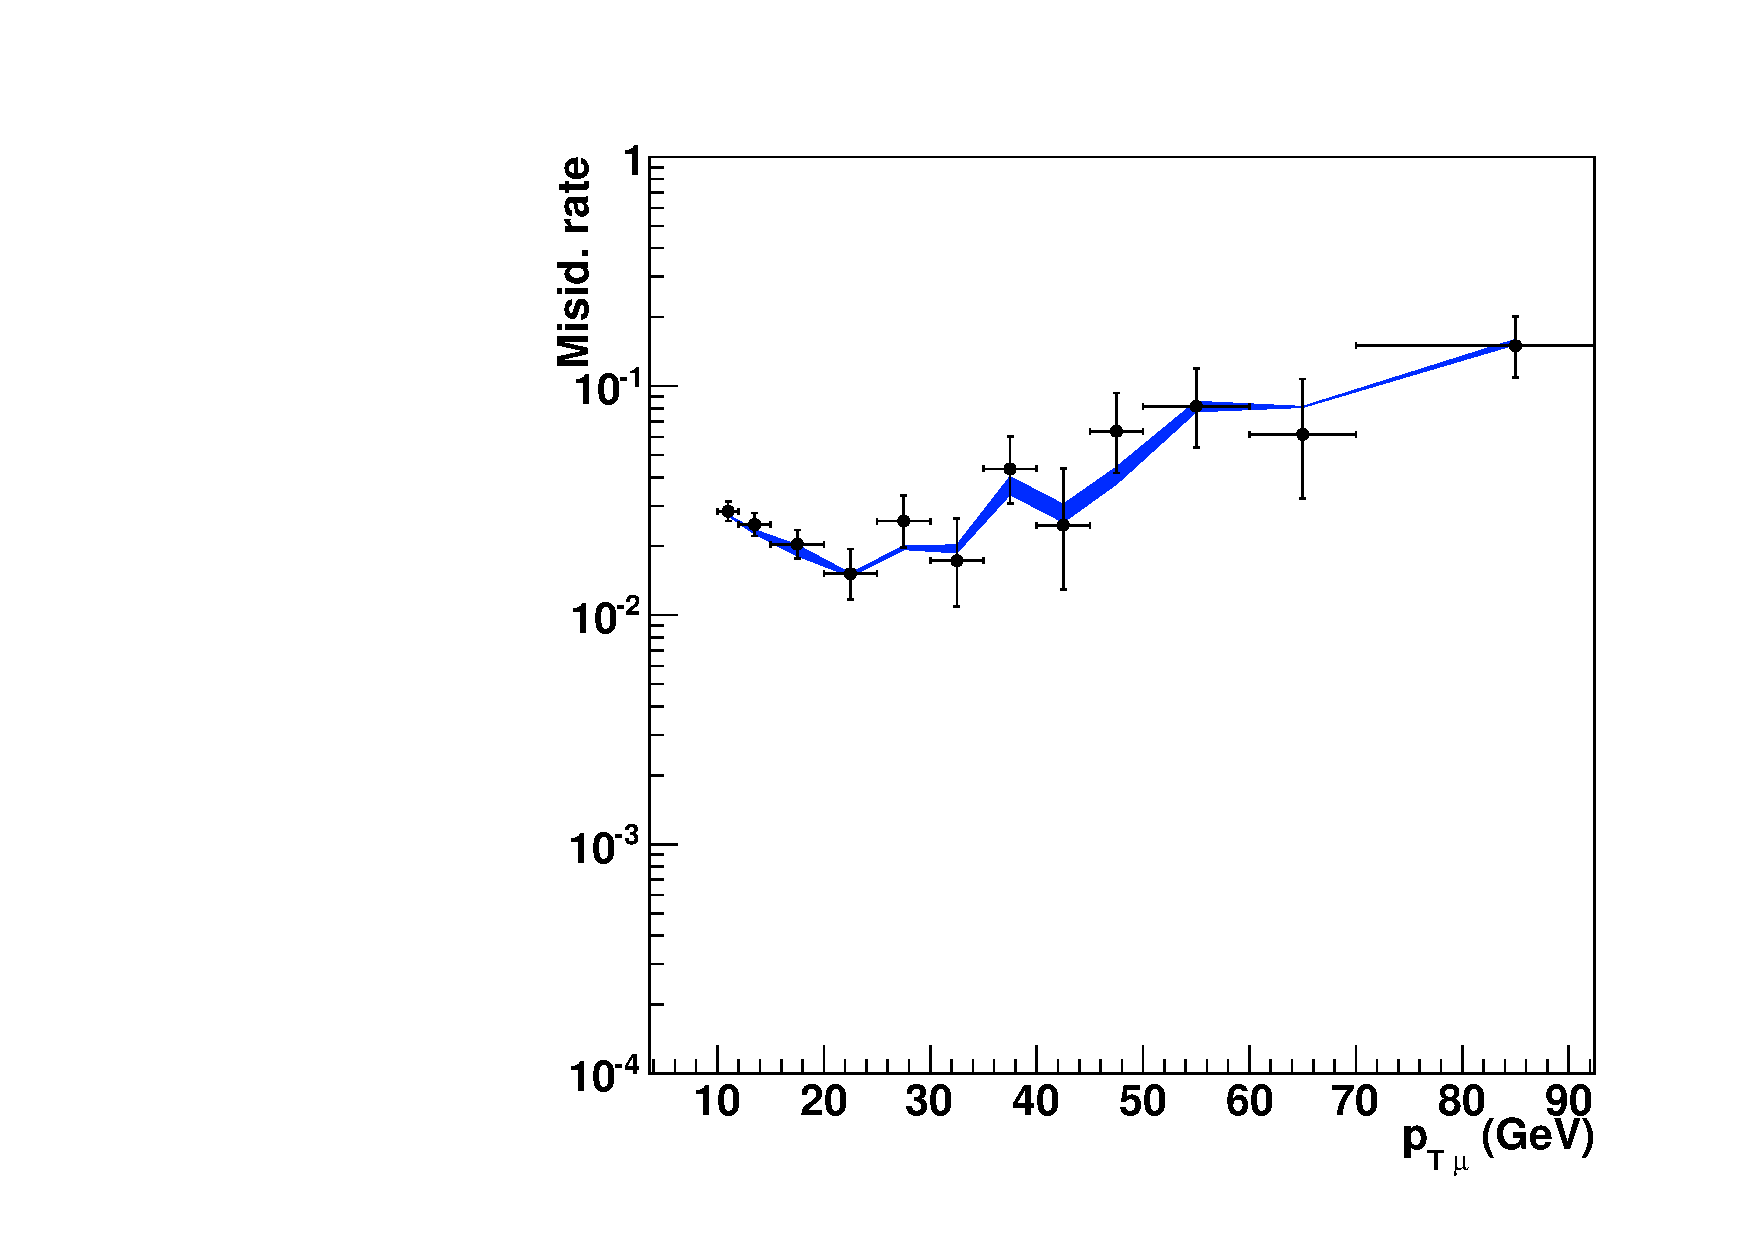
\includegraphics[width=\textwidth]{4_Analisys/pics/8TeV/plots/fakerates/m_emt_kNN_muonPt.pdf}
                \caption{}
        \end{subfigure}
        \begin{subfigure}[b]{0.33\textwidth}
                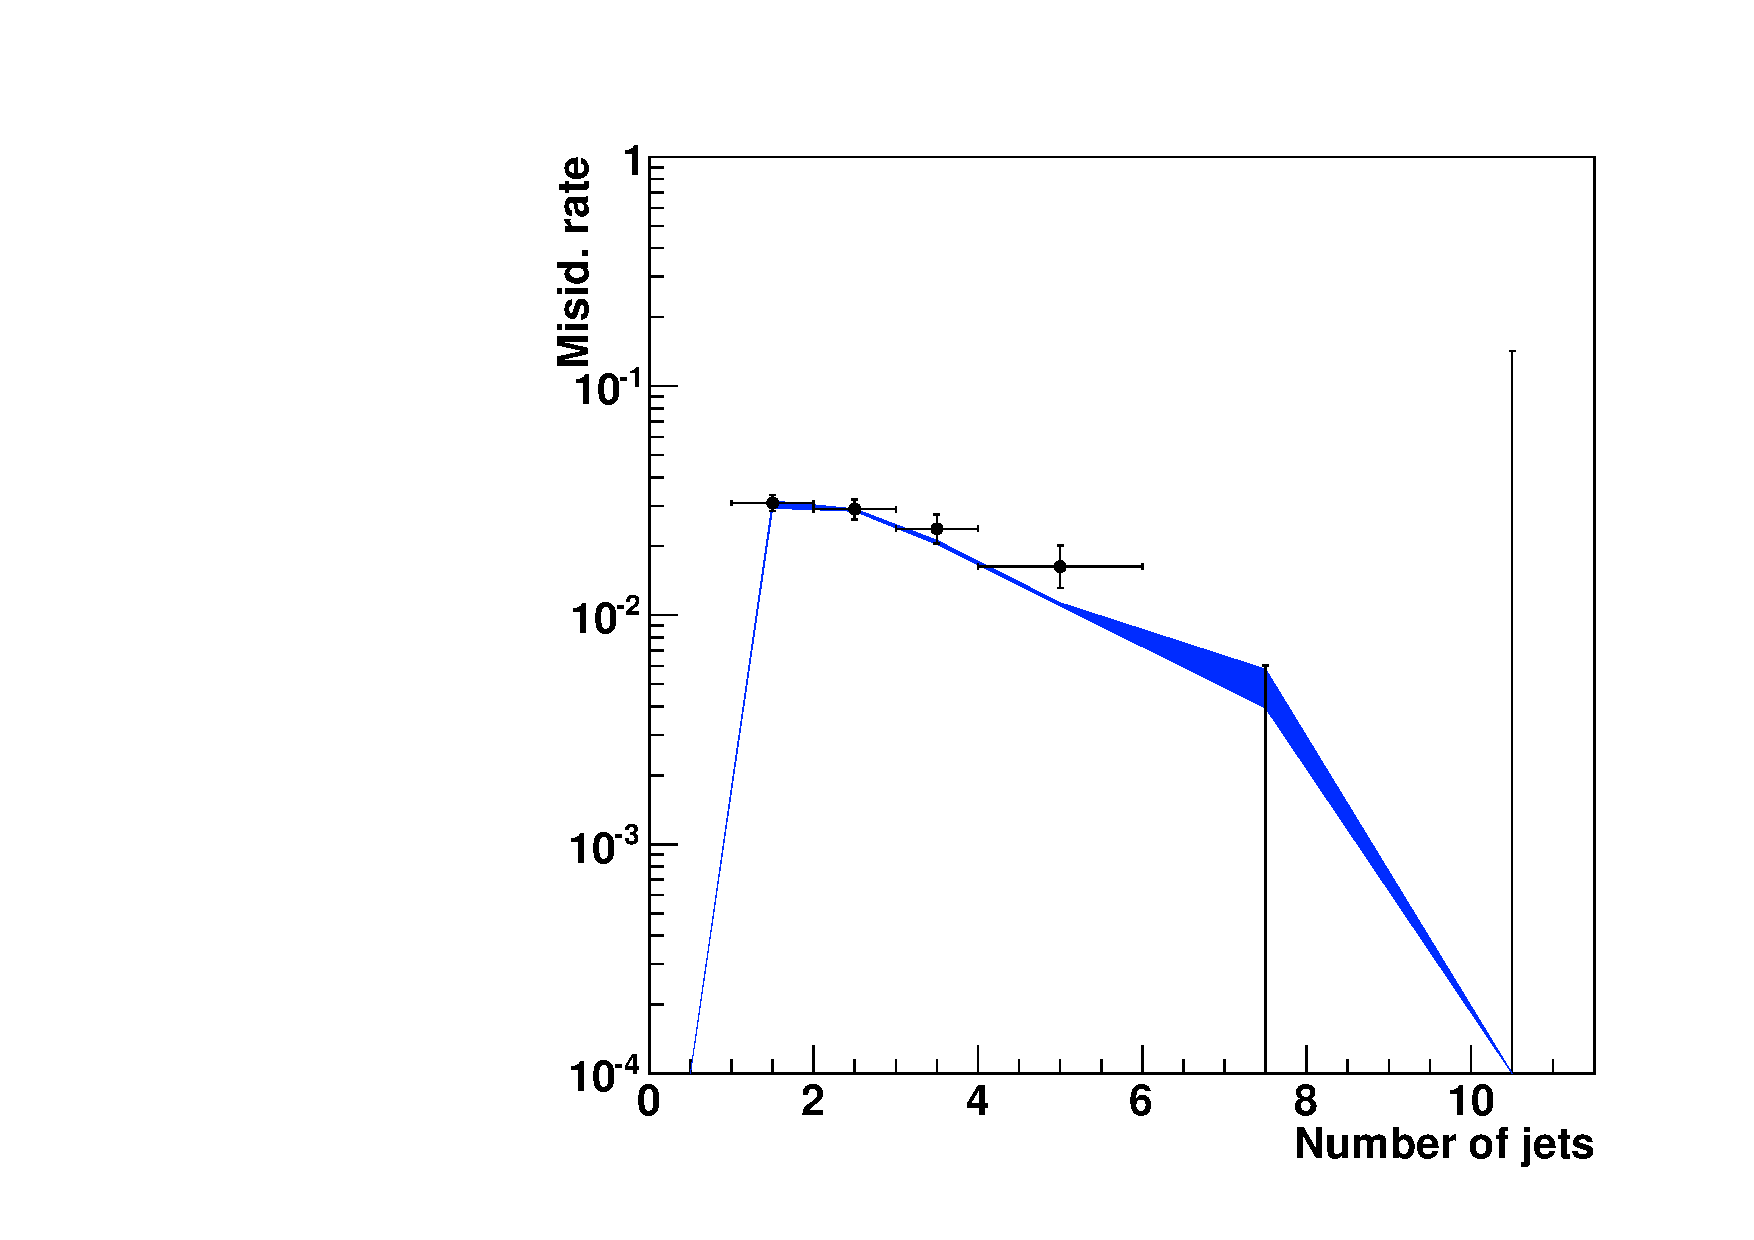
\includegraphics[width=\textwidth]{4_Analisys/pics/8TeV/plots/fakerates/m_emt_kNN_numJets20.pdf}
                \caption{}
        \end{subfigure}

        \begin{subfigure}[b]{0.33\textwidth}
		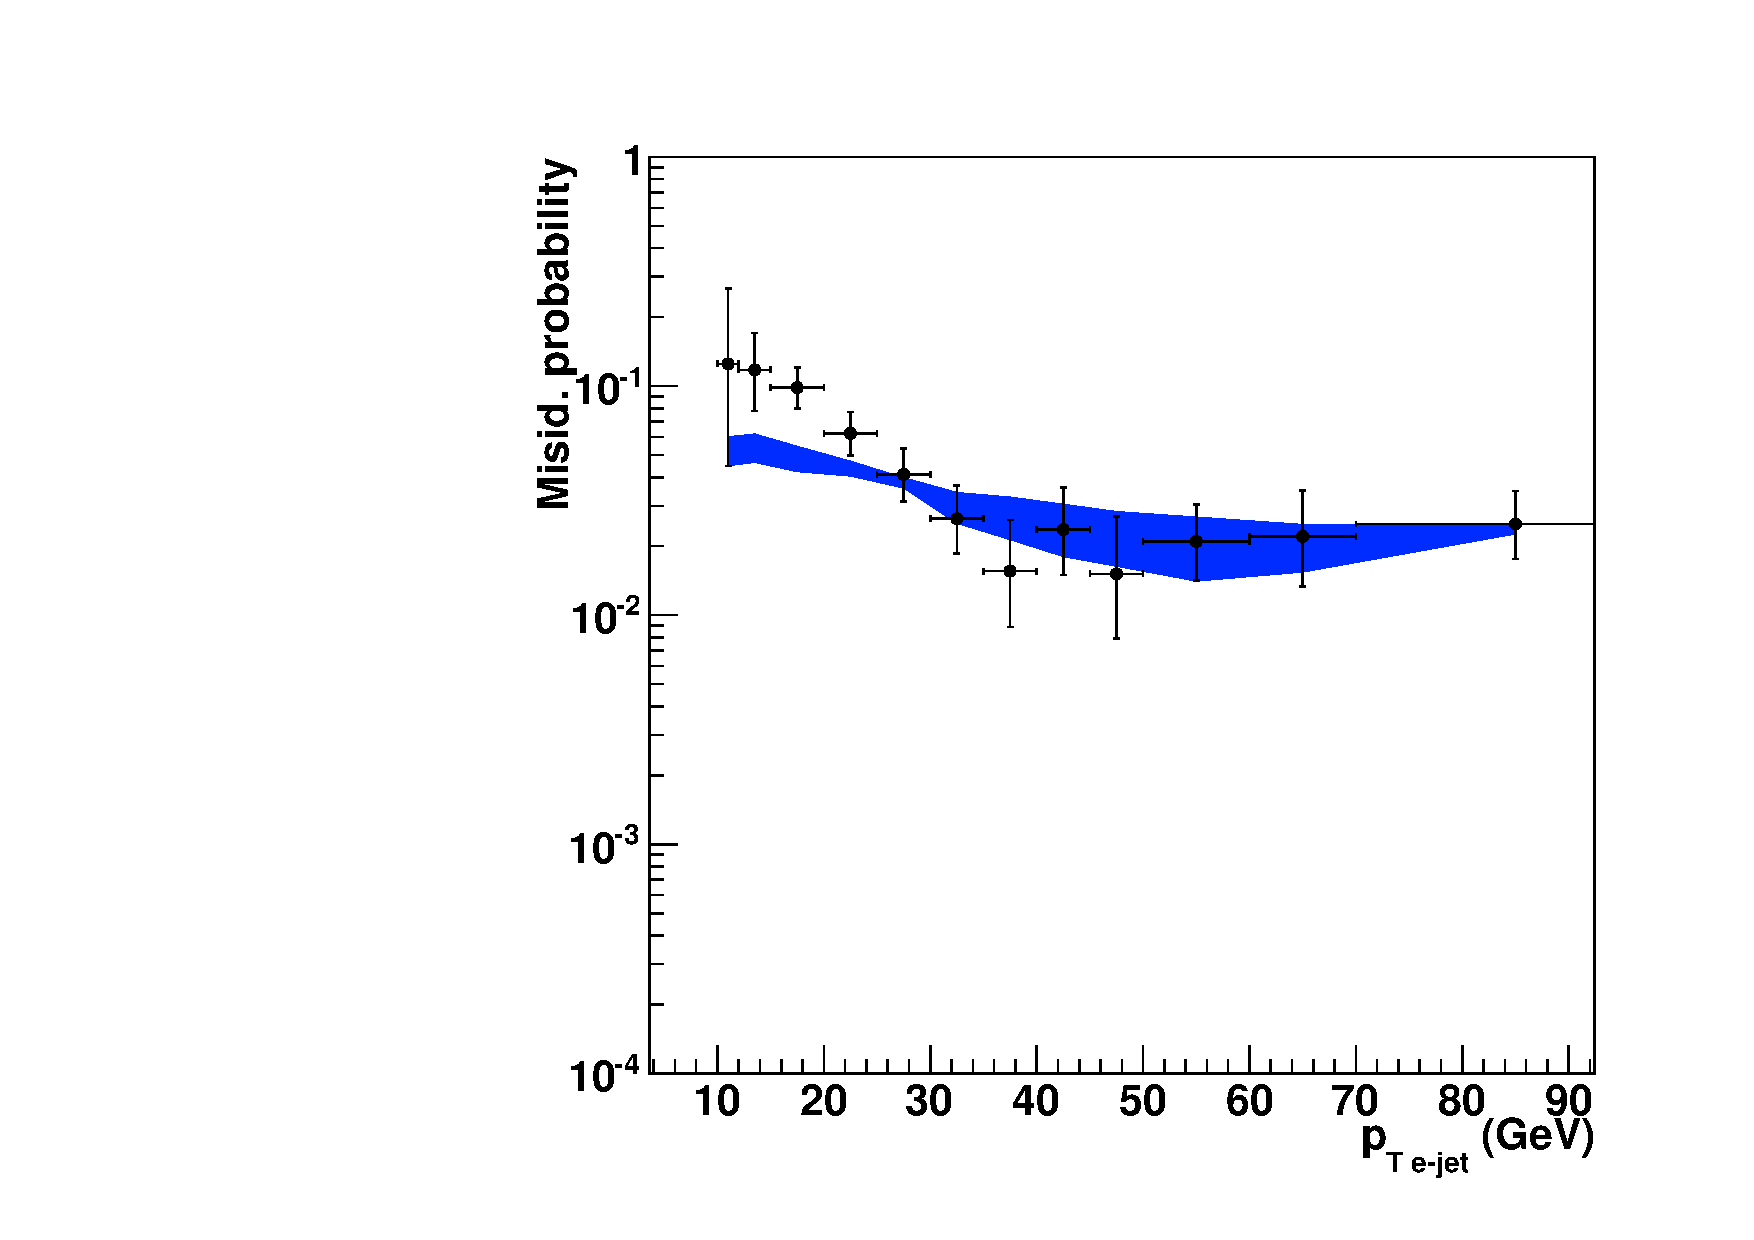
\includegraphics[width=\textwidth]{4_Analisys/pics/8TeV/plots/fakerates/e_emt_kNN_electronJetPt.pdf}
                \caption{}
        \end{subfigure}%
        \begin{subfigure}[b]{0.33\textwidth}
                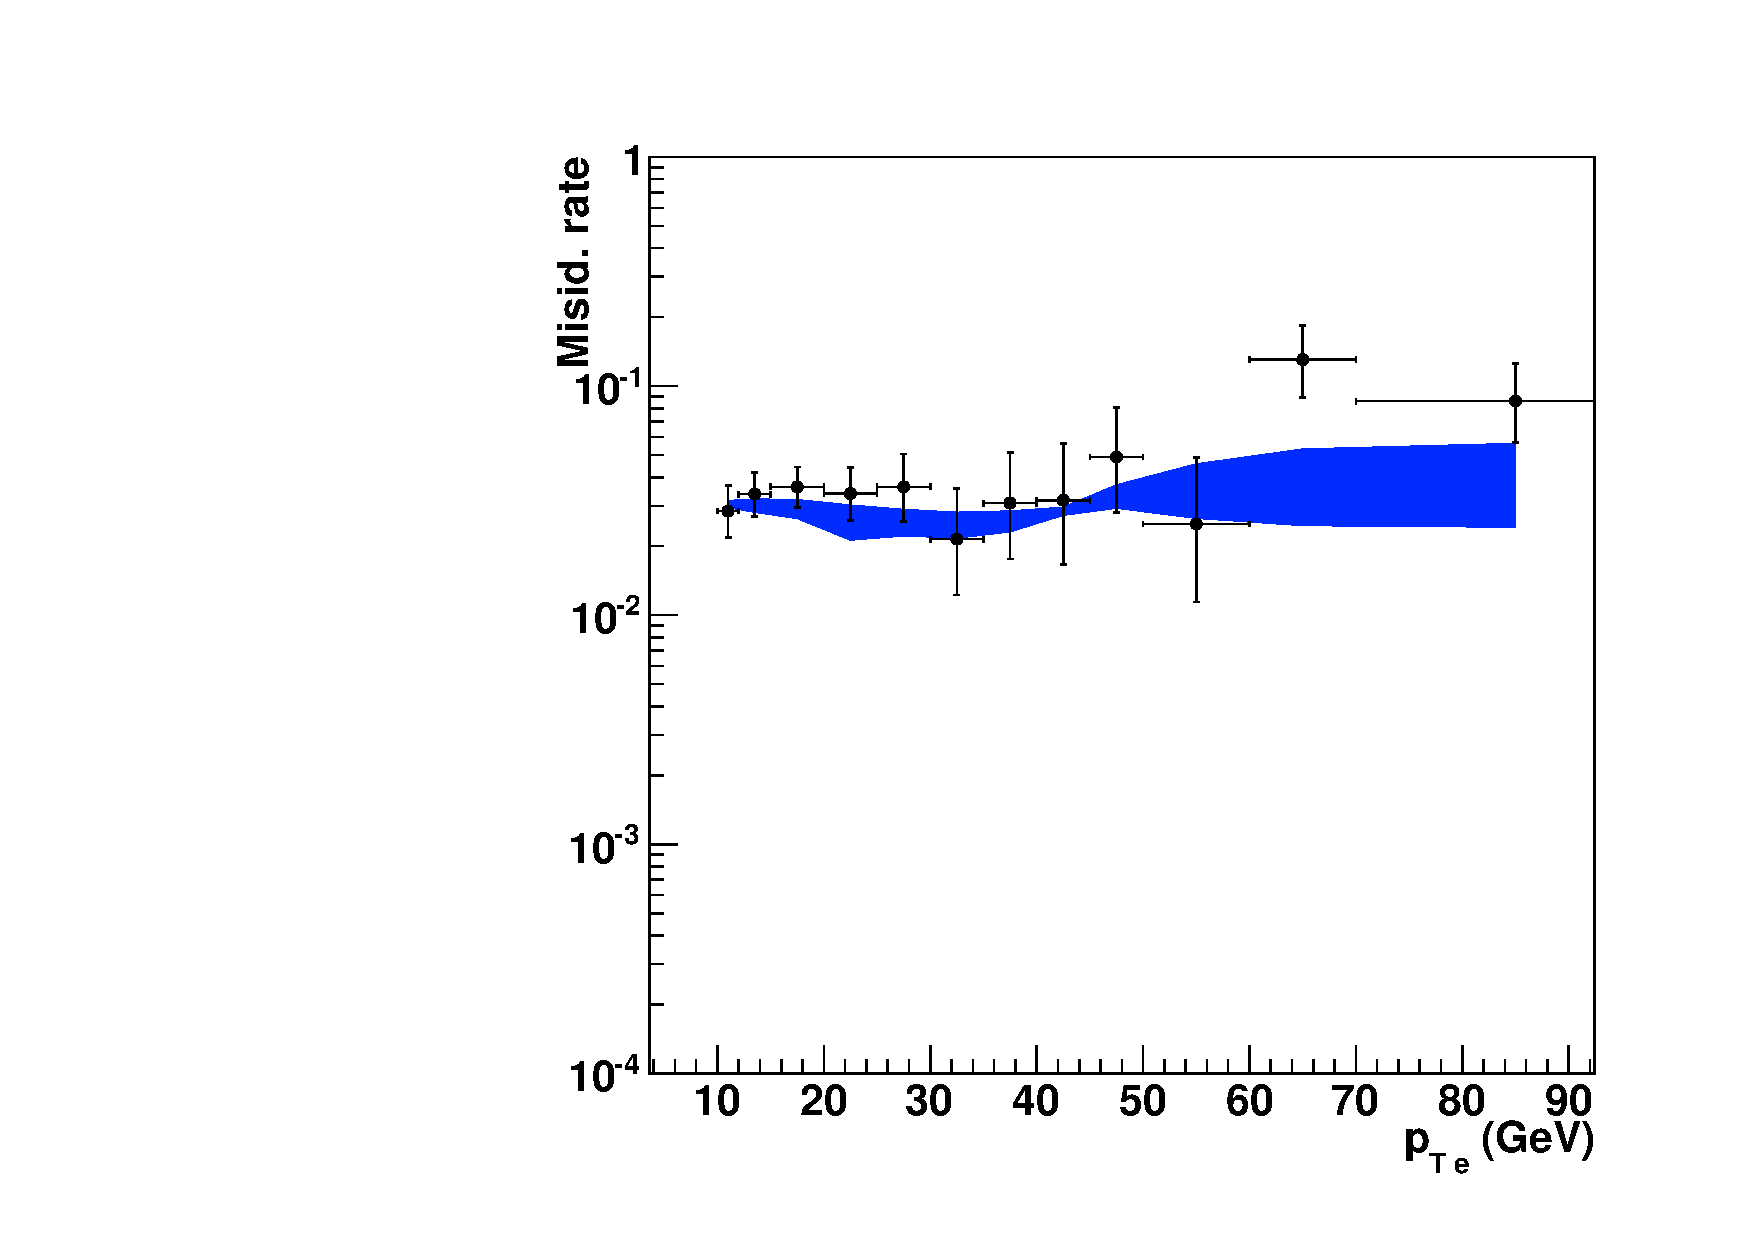
\includegraphics[width=\textwidth]{4_Analisys/pics/8TeV/plots/fakerates/e_emt_kNN_electronPt.pdf}
                \caption{}
        \end{subfigure}
        \begin{subfigure}[b]{0.33\textwidth}
                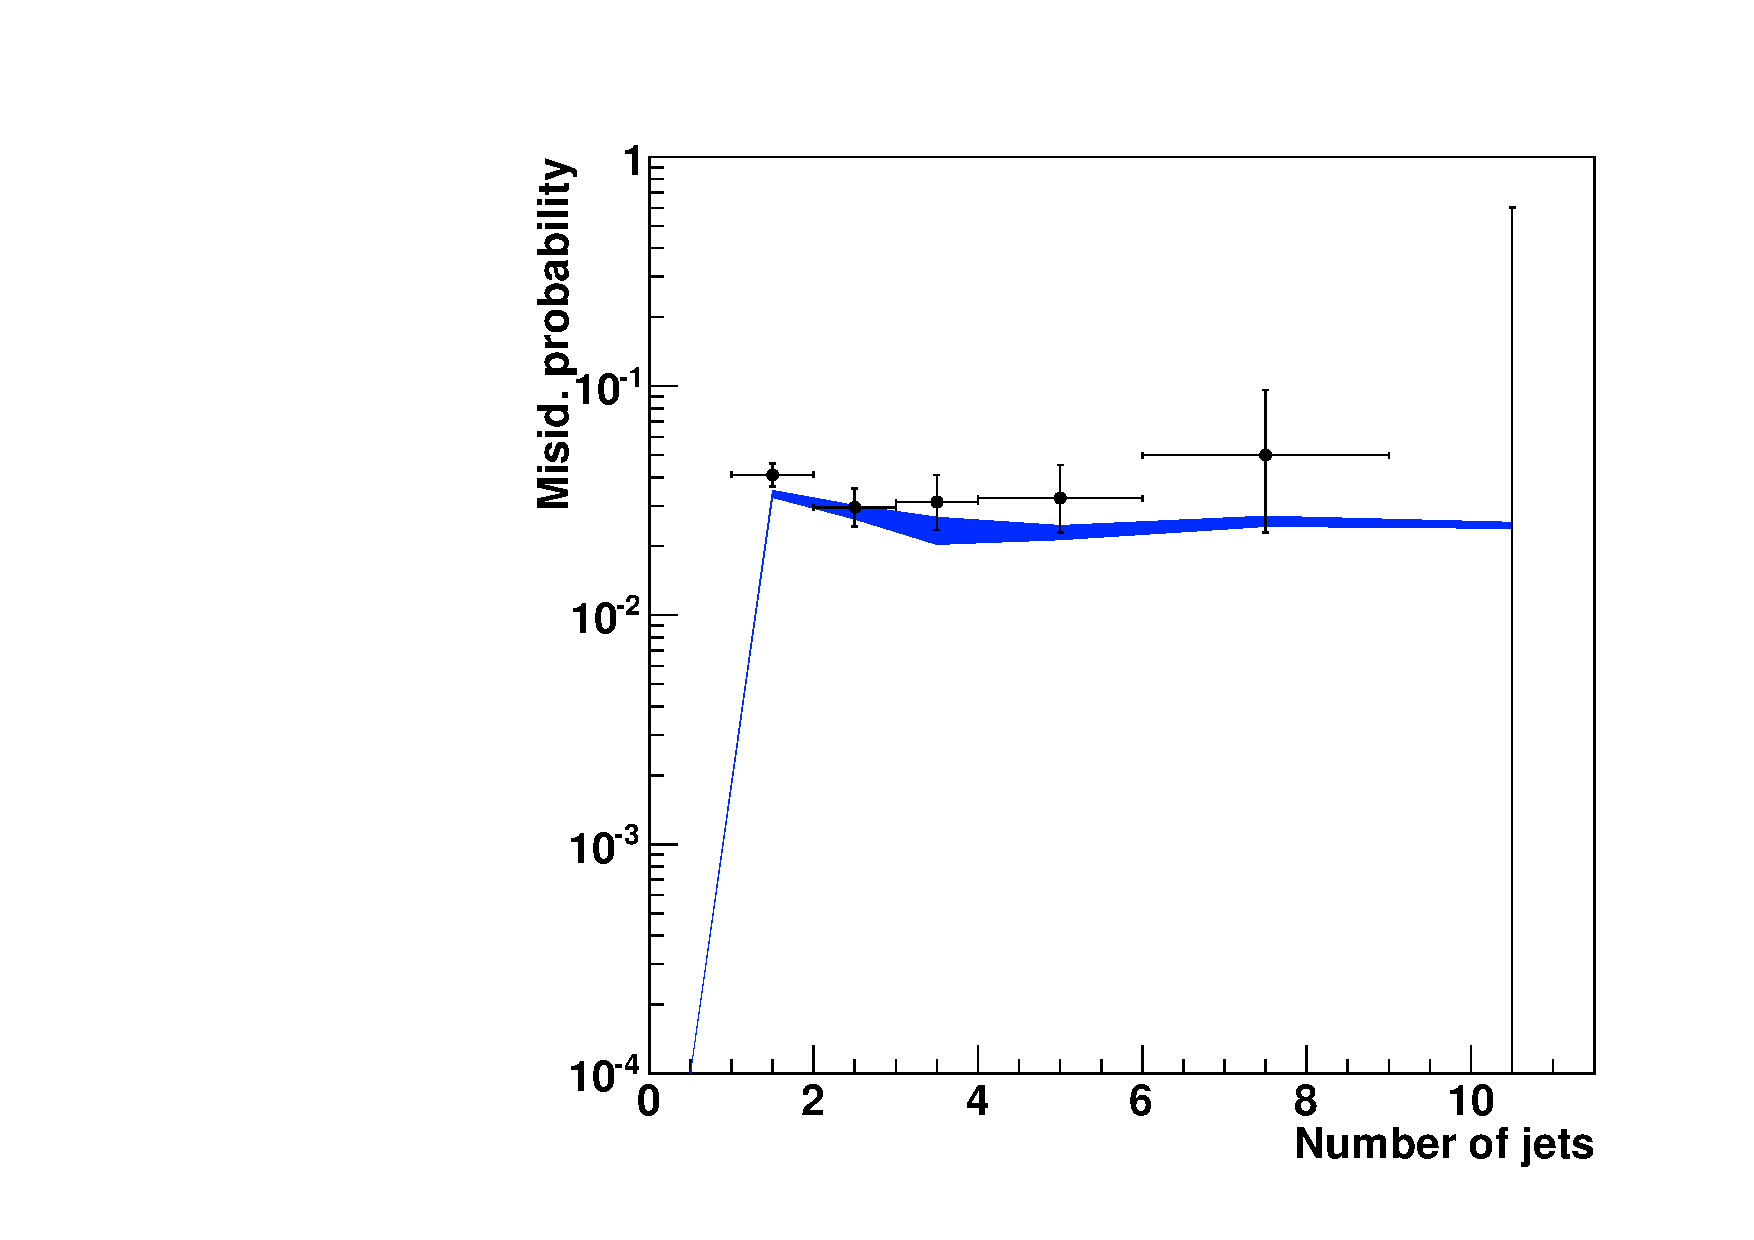
\includegraphics[width=\textwidth]{4_Analisys/pics/8TeV/plots/fakerates/e_emt_kNN_numJets20.pdf}
                \caption{}
        \end{subfigure}
        \caption{Measured misidentification probability for muons (top) and electrons (bottom) in the training sample dedicated to the $e\mu\tau_h$ channel. The blue band represents the output of the kNN algorithm and its related uncertainty.}\label{fig:fake_rate_emt}
\end{figure}

\begin{figure}
        \centering
        \begin{subfigure}[b]{0.33\textwidth}
		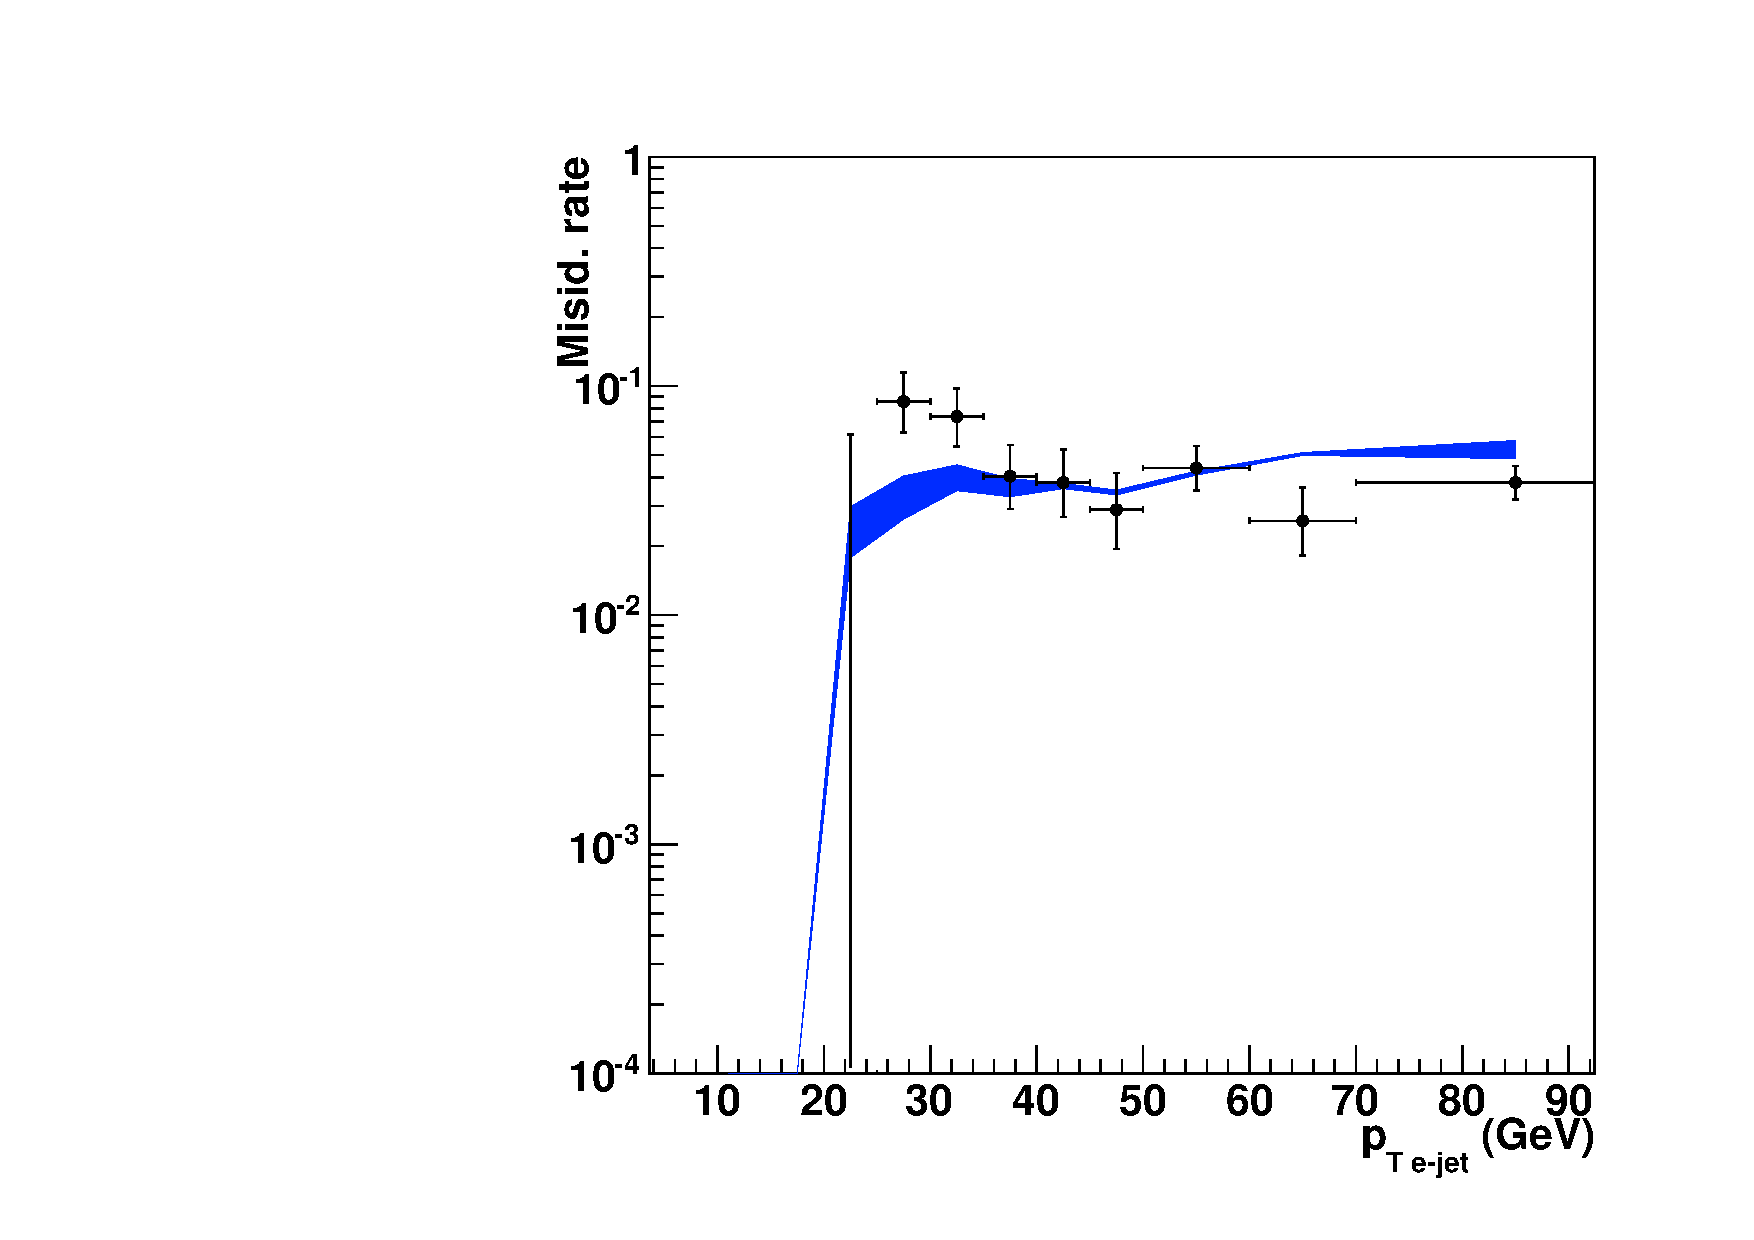
\includegraphics[width=\textwidth]{4_Analisys/pics/8TeV/plots/fakerates/e_eet_leading_kNN_electronJetPt.pdf}
                \caption{}
        \end{subfigure}%
        \begin{subfigure}[b]{0.33\textwidth}
                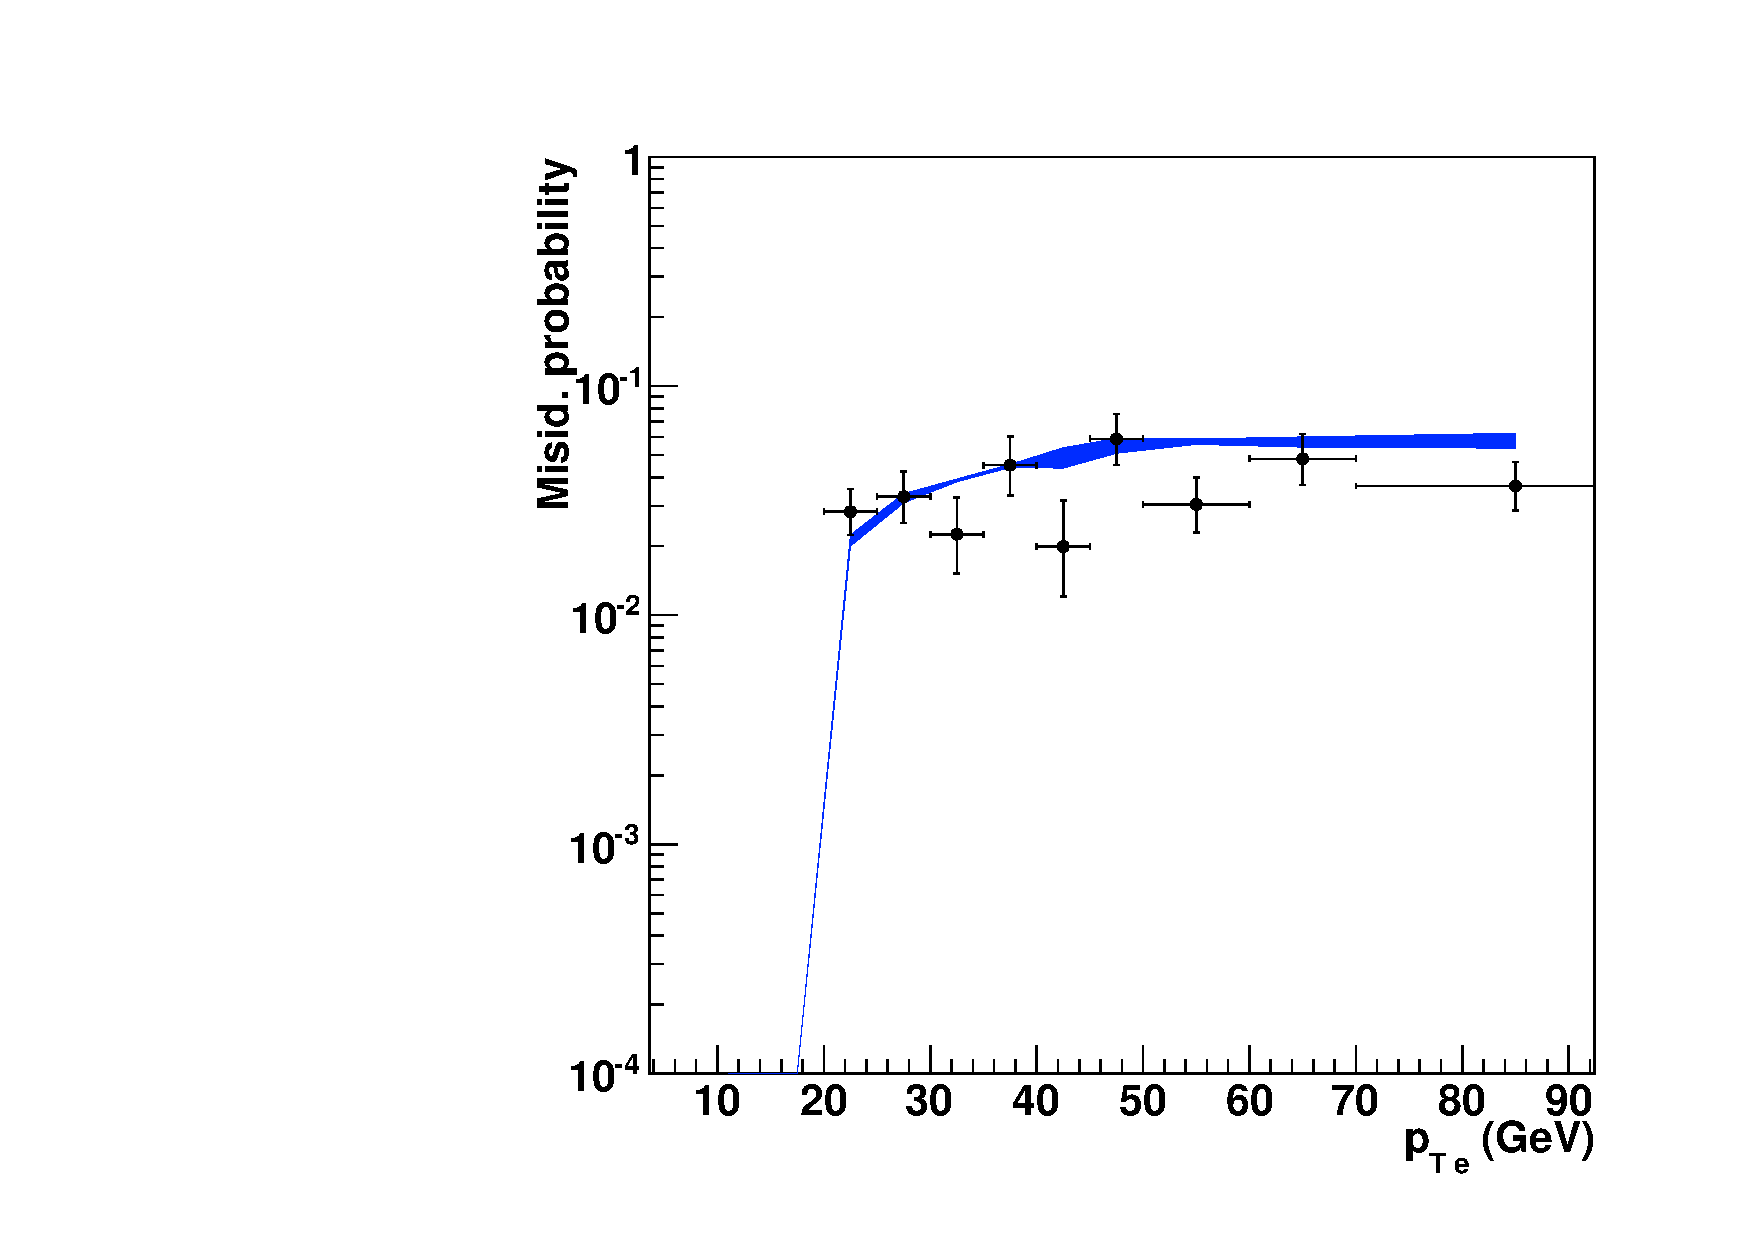
\includegraphics[width=\textwidth]{4_Analisys/pics/8TeV/plots/fakerates/e_eet_leading_kNN_electronPt.pdf}
                \caption{}
        \end{subfigure}
        \begin{subfigure}[b]{0.33\textwidth}
                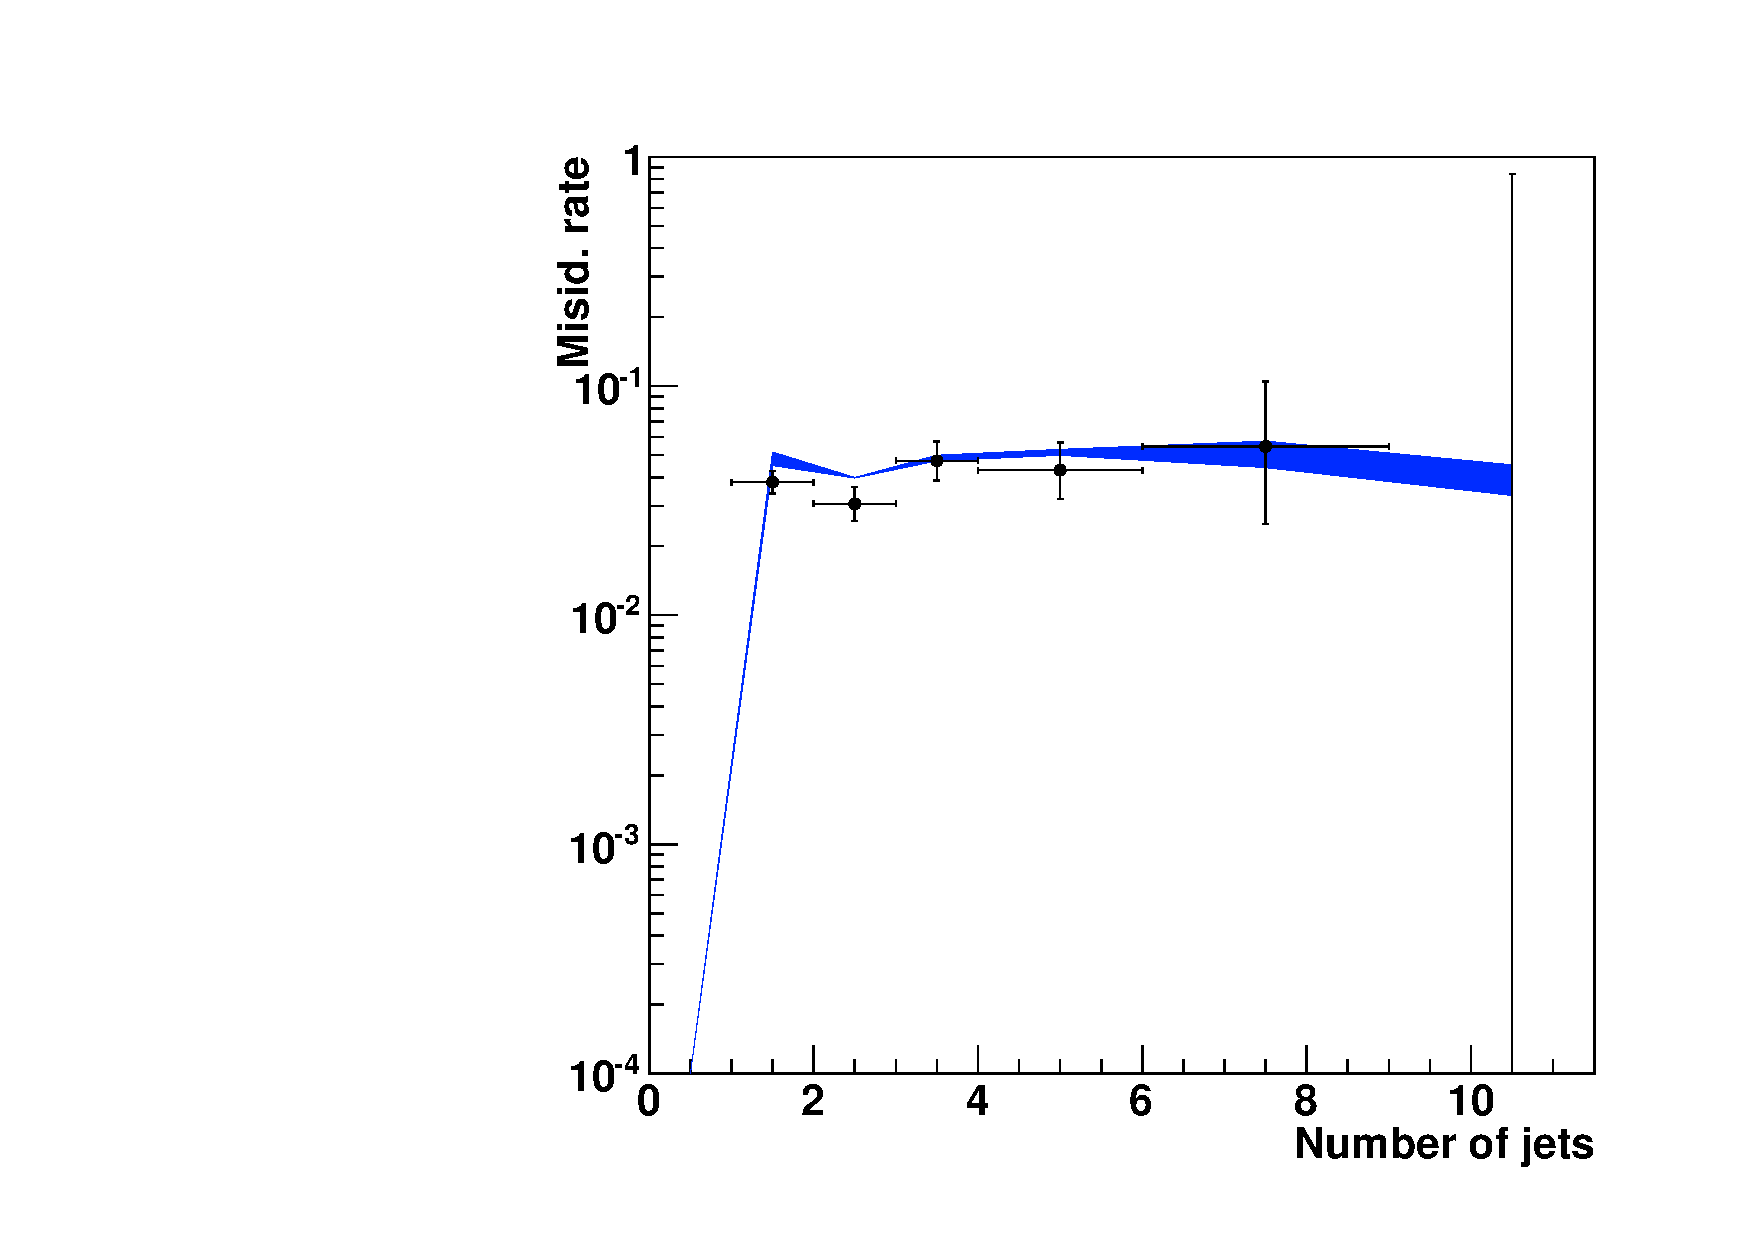
\includegraphics[width=\textwidth]{4_Analisys/pics/8TeV/plots/fakerates/e_eet_leading_kNN_numJets20.pdf}
                \caption{}
        \end{subfigure}

        \begin{subfigure}[b]{0.33\textwidth}
		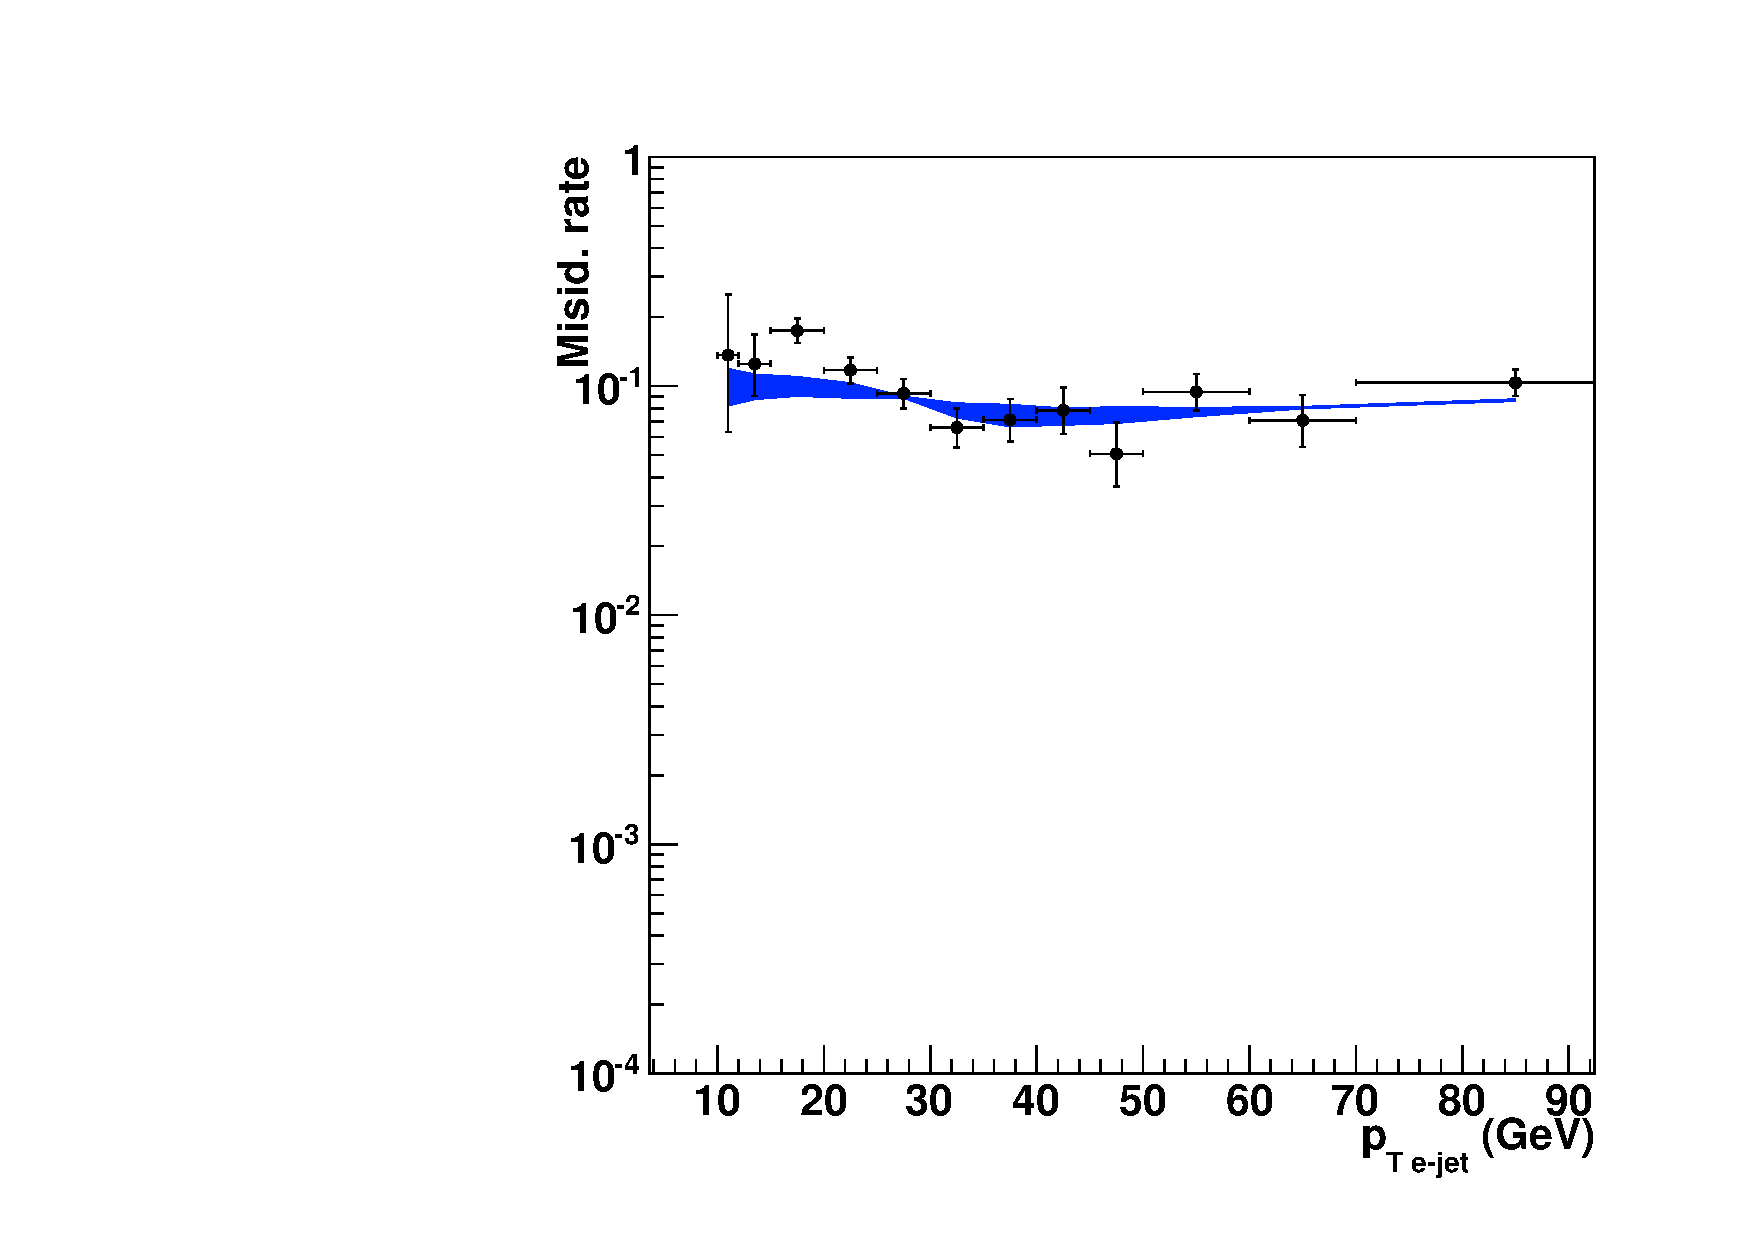
\includegraphics[width=\textwidth]{4_Analisys/pics/8TeV/plots/fakerates/e_eet_subleading_kNN_electronJetPt.pdf}
                \caption{}
        \end{subfigure}%
        \begin{subfigure}[b]{0.33\textwidth}
                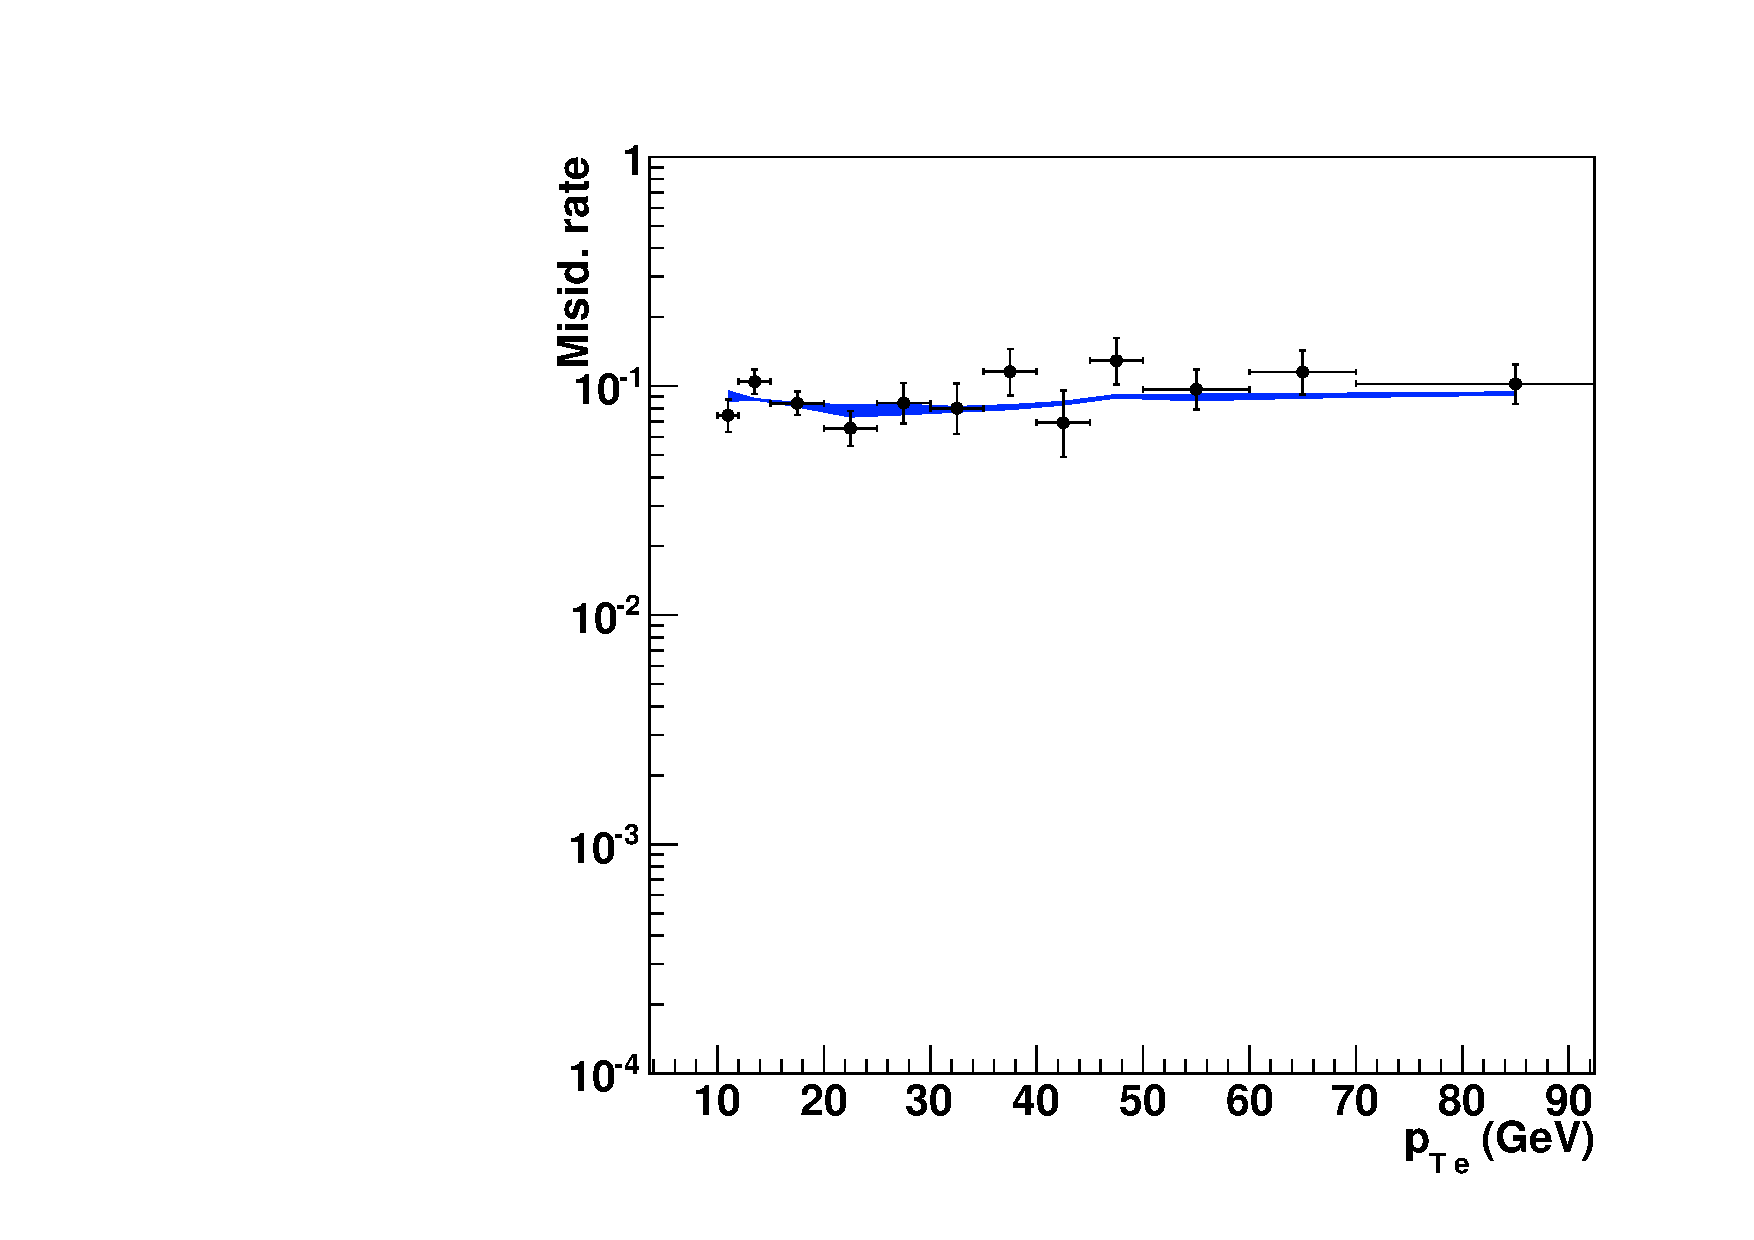
\includegraphics[width=\textwidth]{4_Analisys/pics/8TeV/plots/fakerates/e_eet_subleading_kNN_electronPt.pdf}
                \caption{}
        \end{subfigure}
        \begin{subfigure}[b]{0.33\textwidth}
                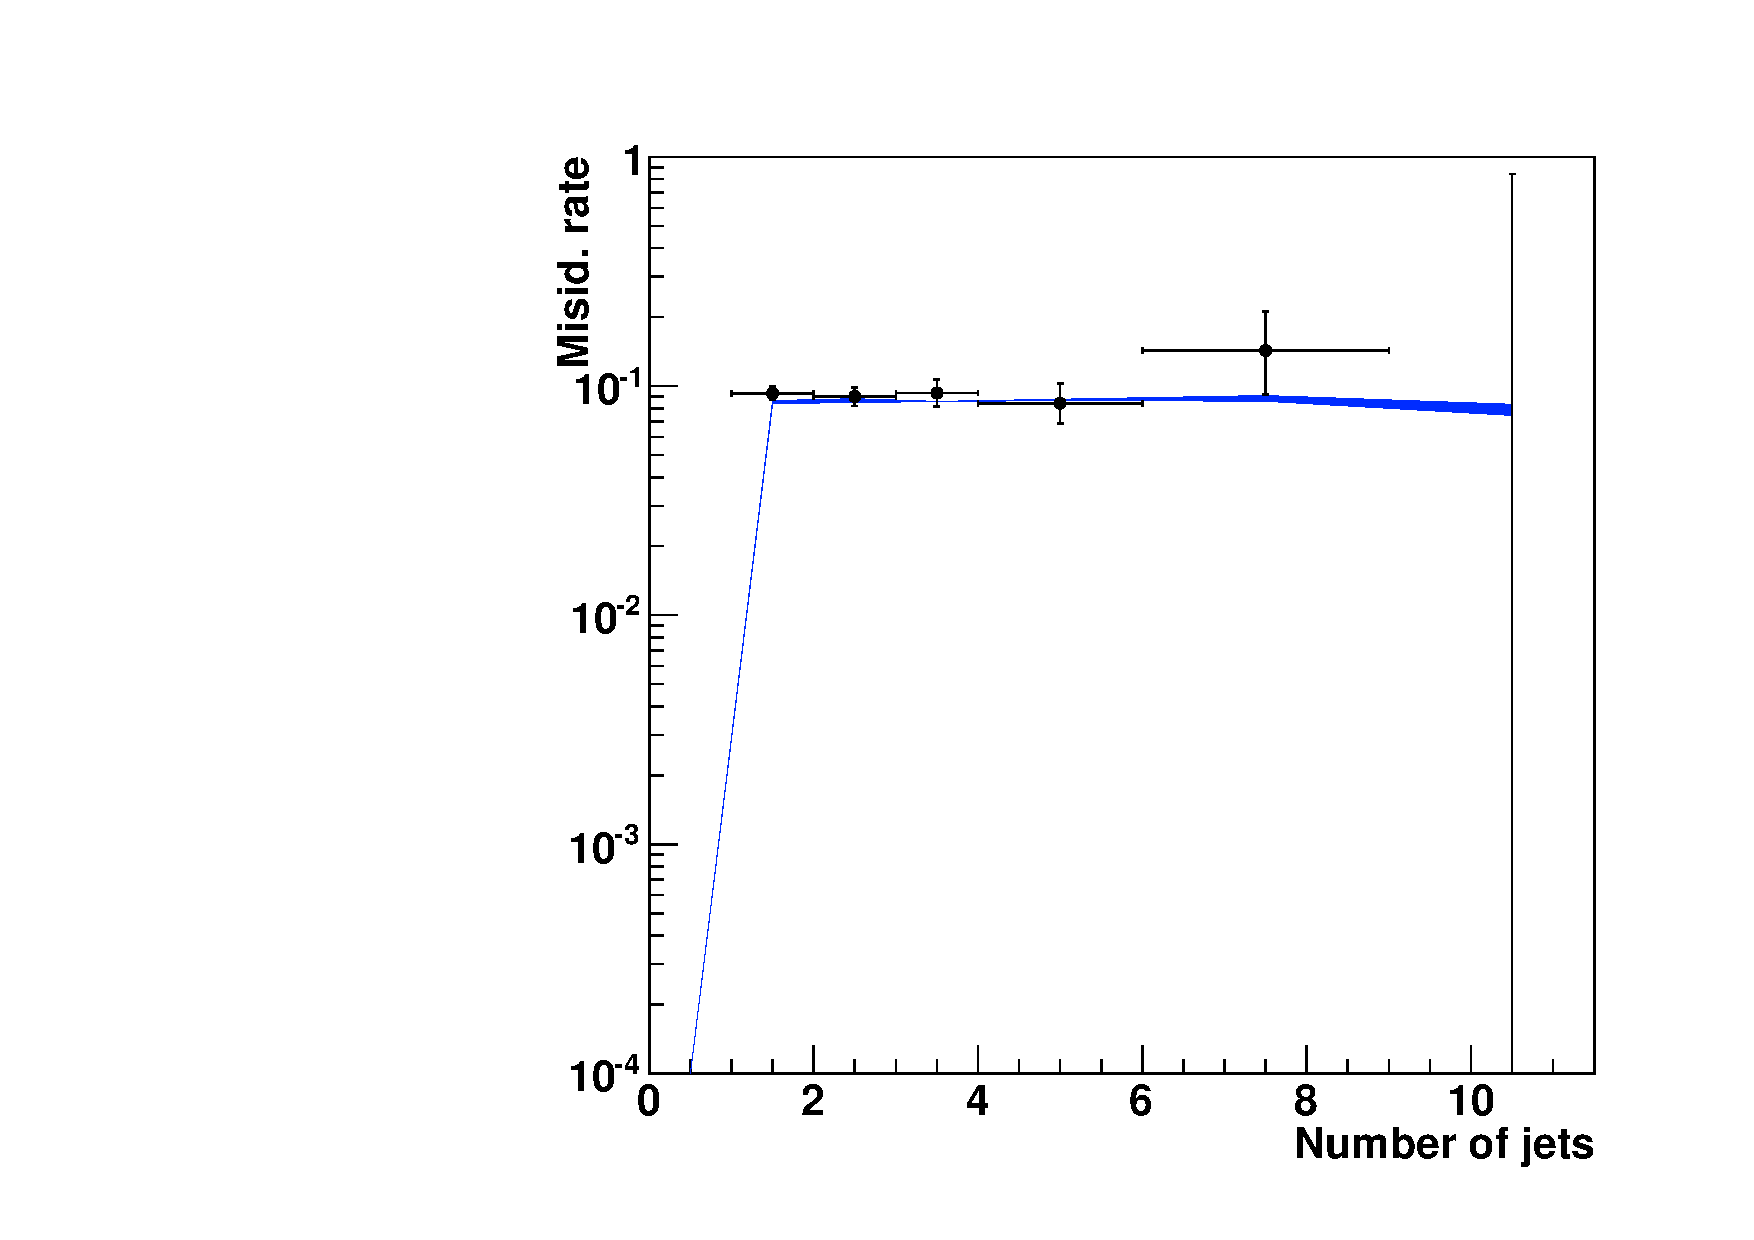
\includegraphics[width=\textwidth]{4_Analisys/pics/8TeV/plots/fakerates/e_eet_subleading_kNN_numJets20.pdf}
                \caption{}
        \end{subfigure}
        \caption{Measured misidentification probability for leading (top) and sub-leading (bottom) electrons in the training sample dedicated to the $ee\tau_h$ channel. The blue band represents the output of the kNN algorithm and its related uncertainty.}\label{fig:fake_rate_eet}
\end{figure}

\section{Background control regions}

Figures~\ref{fig:LLT_mmt_f3_charge3_control_7TeV}--\ref{fig:LLT_eet_f3_charge3_control_8TeV} show the agreement obtained in the control regions with same selection as the signal region but inverted tau isolation and with the requirements that the three objects have the same measured electric charge.

It can be noted that the population of this region is inferior to the one shown in the section~\ref{sec:f3_validation} as the contribution from Z+jets and $t\bar{t}$ is absent in this region, which is also the cause for the slightly worse agreement between observed data and expected backgrounds.

\begin{figure}
\begin{center}
  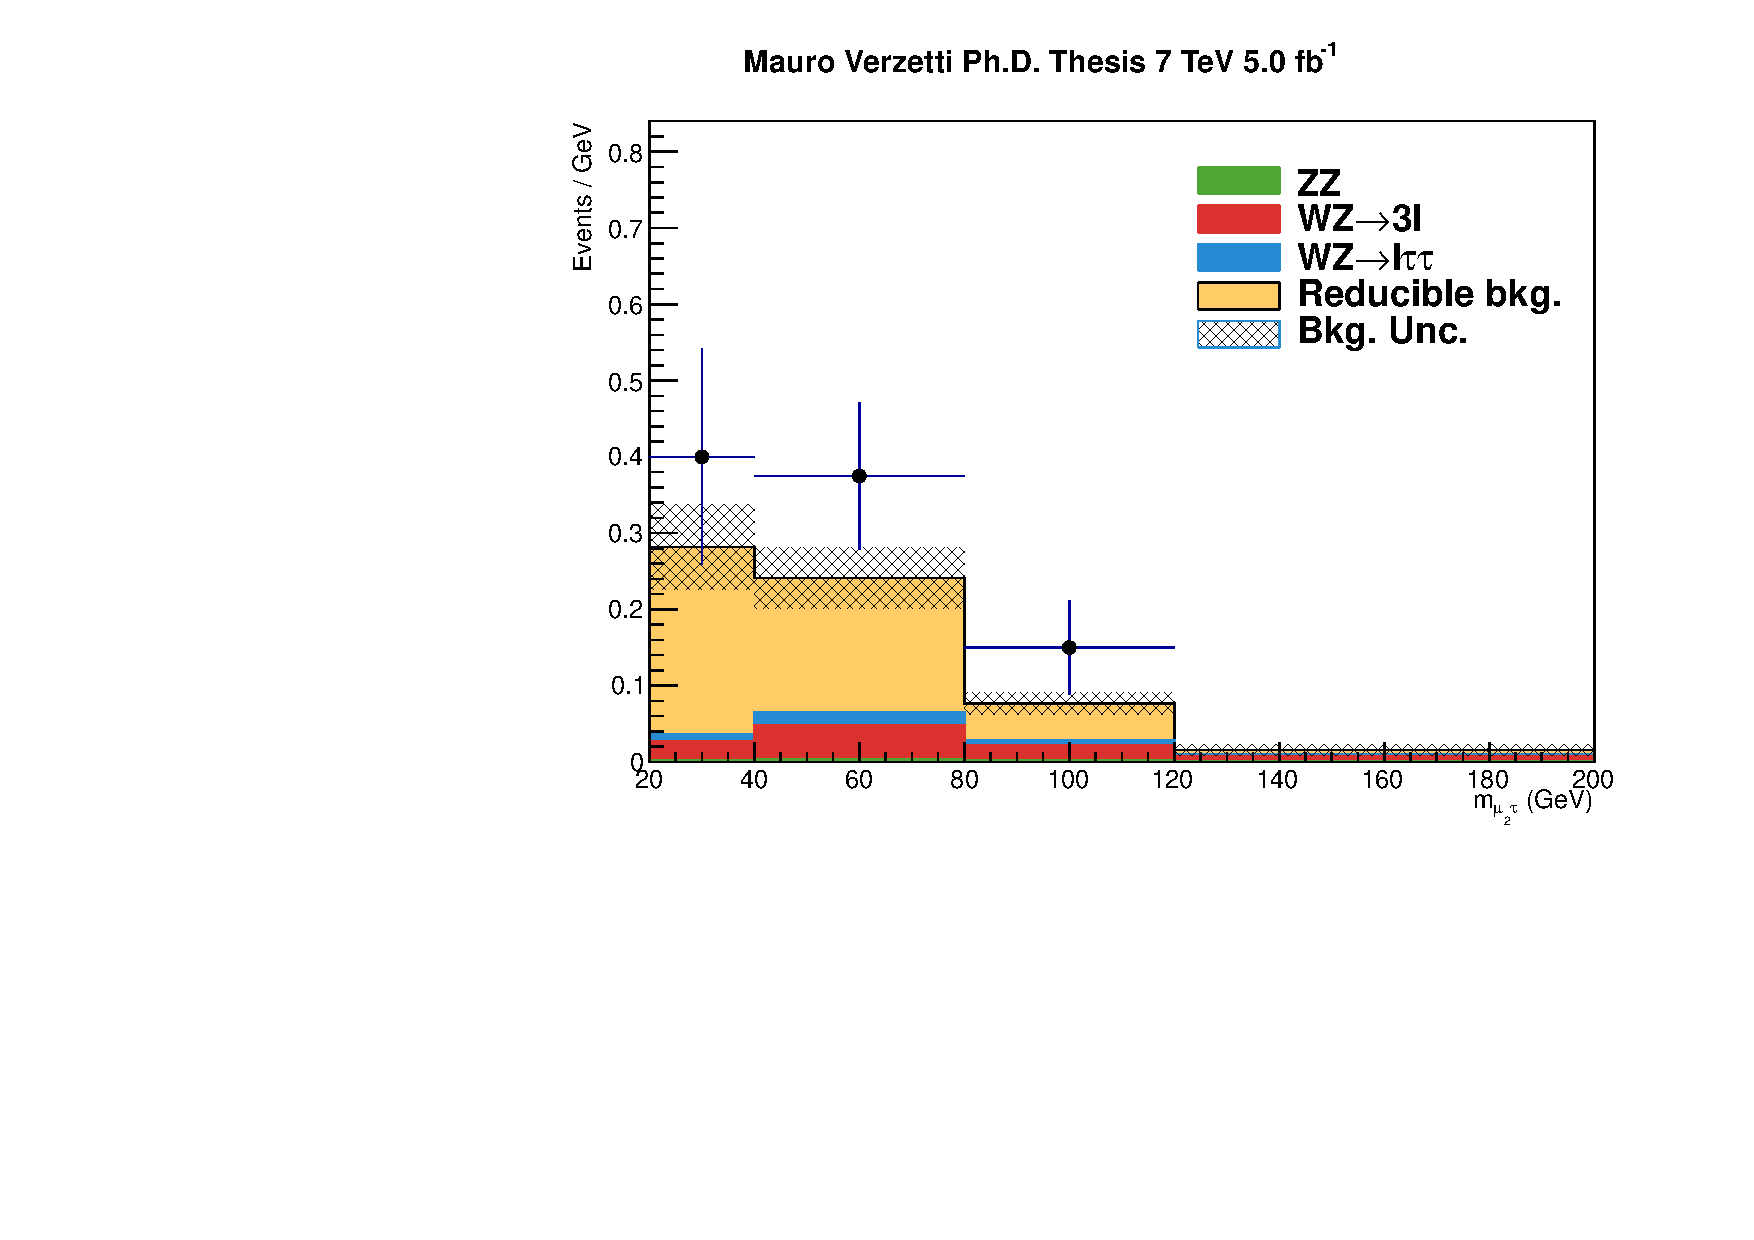
\includegraphics[width=0.49\textwidth]{4_Analisys/pics/7TeV/plots/mmt/f3/Full_charge3/final-f3-subMass-Full.pdf}
  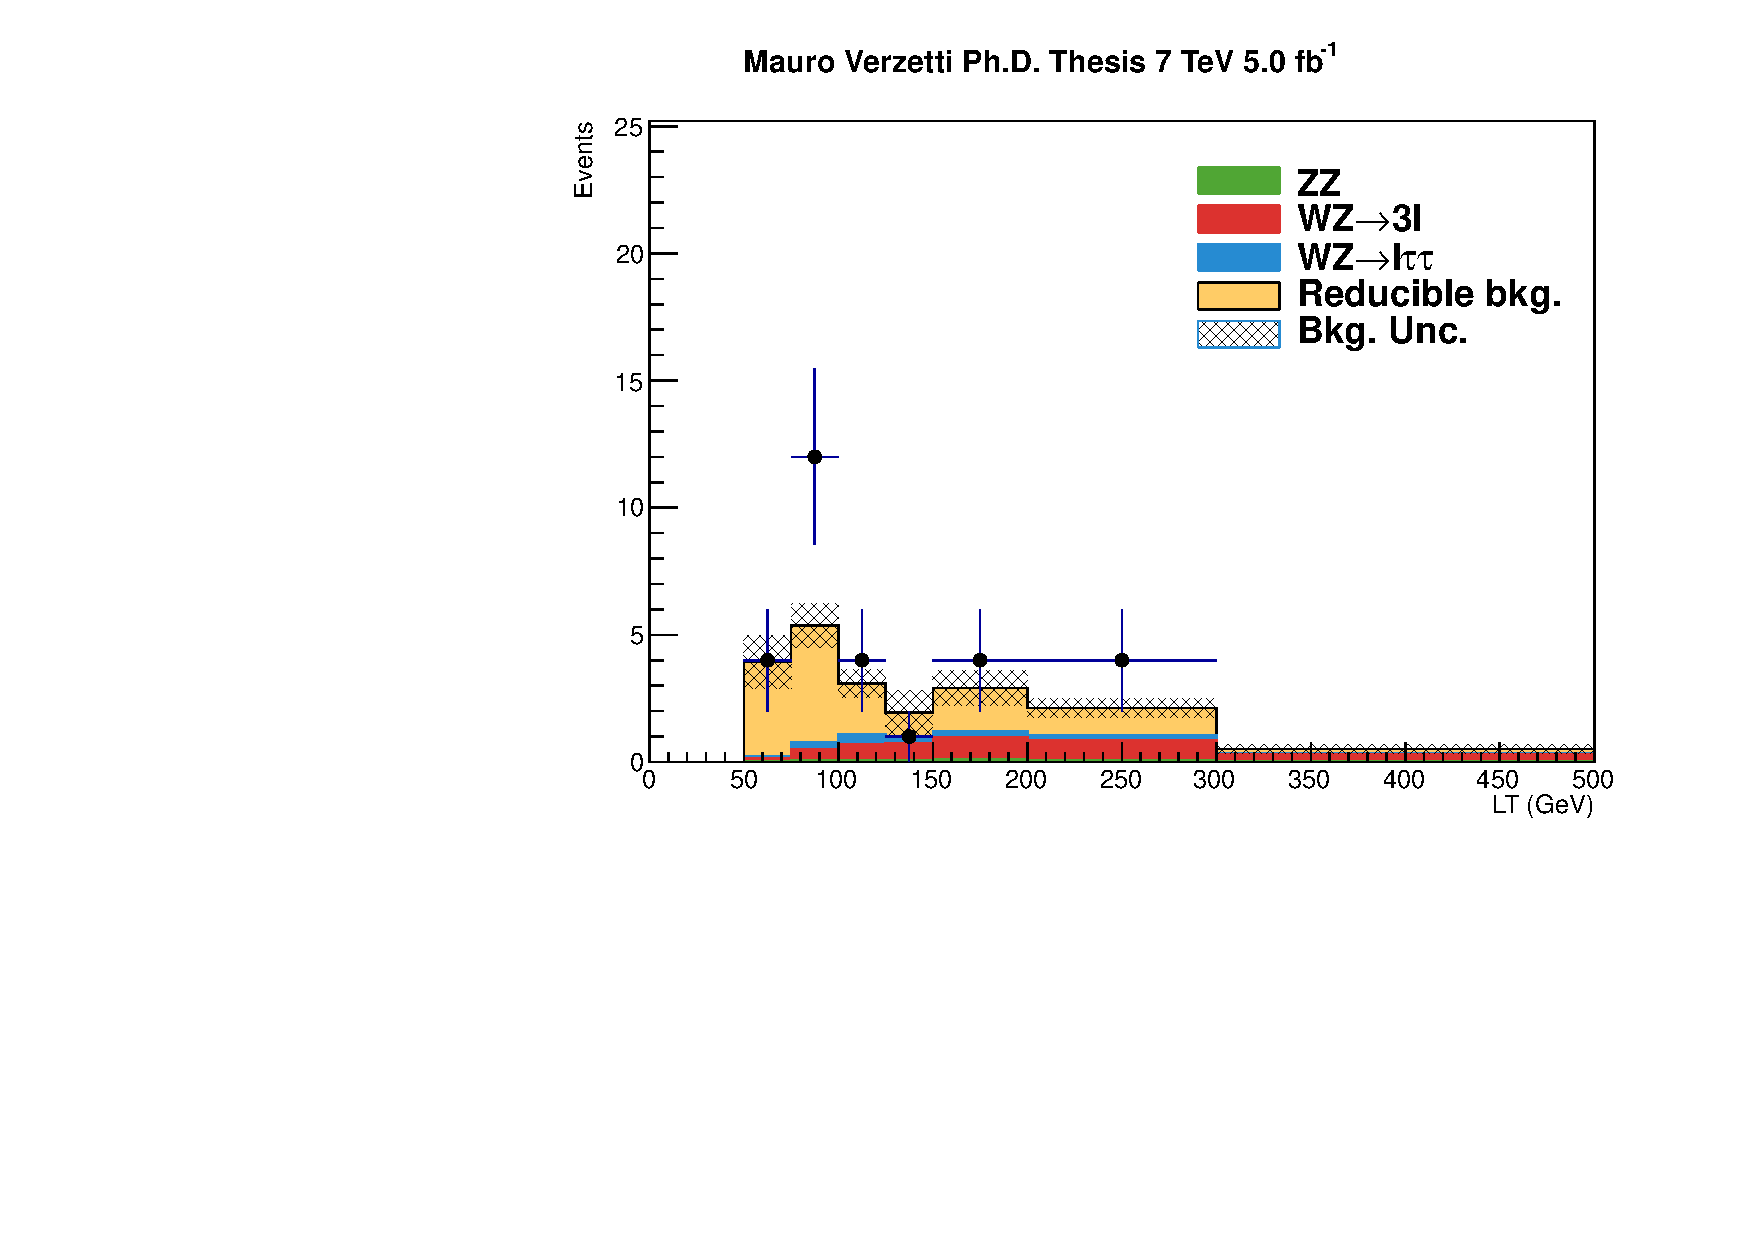
\includegraphics[width=0.49\textwidth]{4_Analisys/pics/7TeV/plots/mmt/f3/final-LT-charge3.pdf}\\
  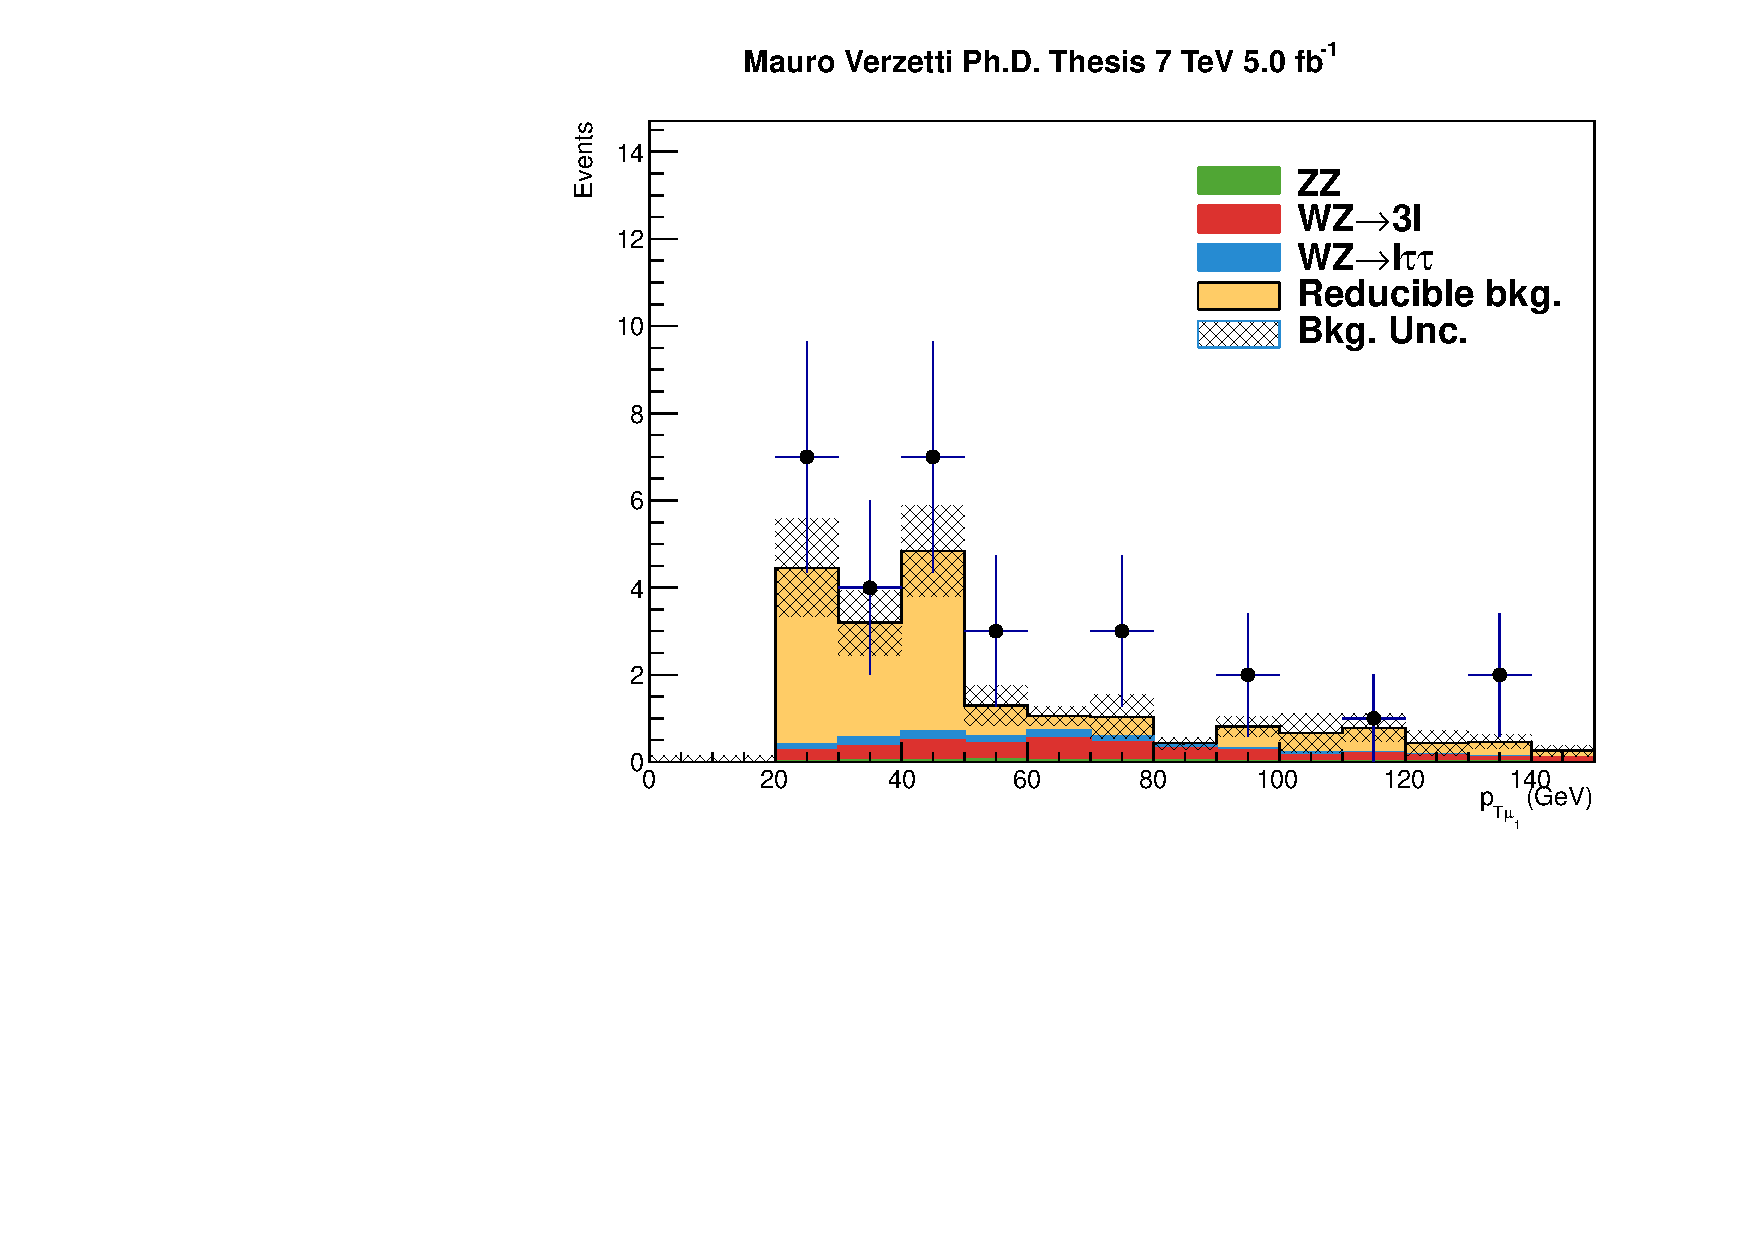
\includegraphics[width=0.49\textwidth]{4_Analisys/pics/7TeV/plots/mmt/f3/Full_charge3/final-f3-m1Pt-Full.pdf}
  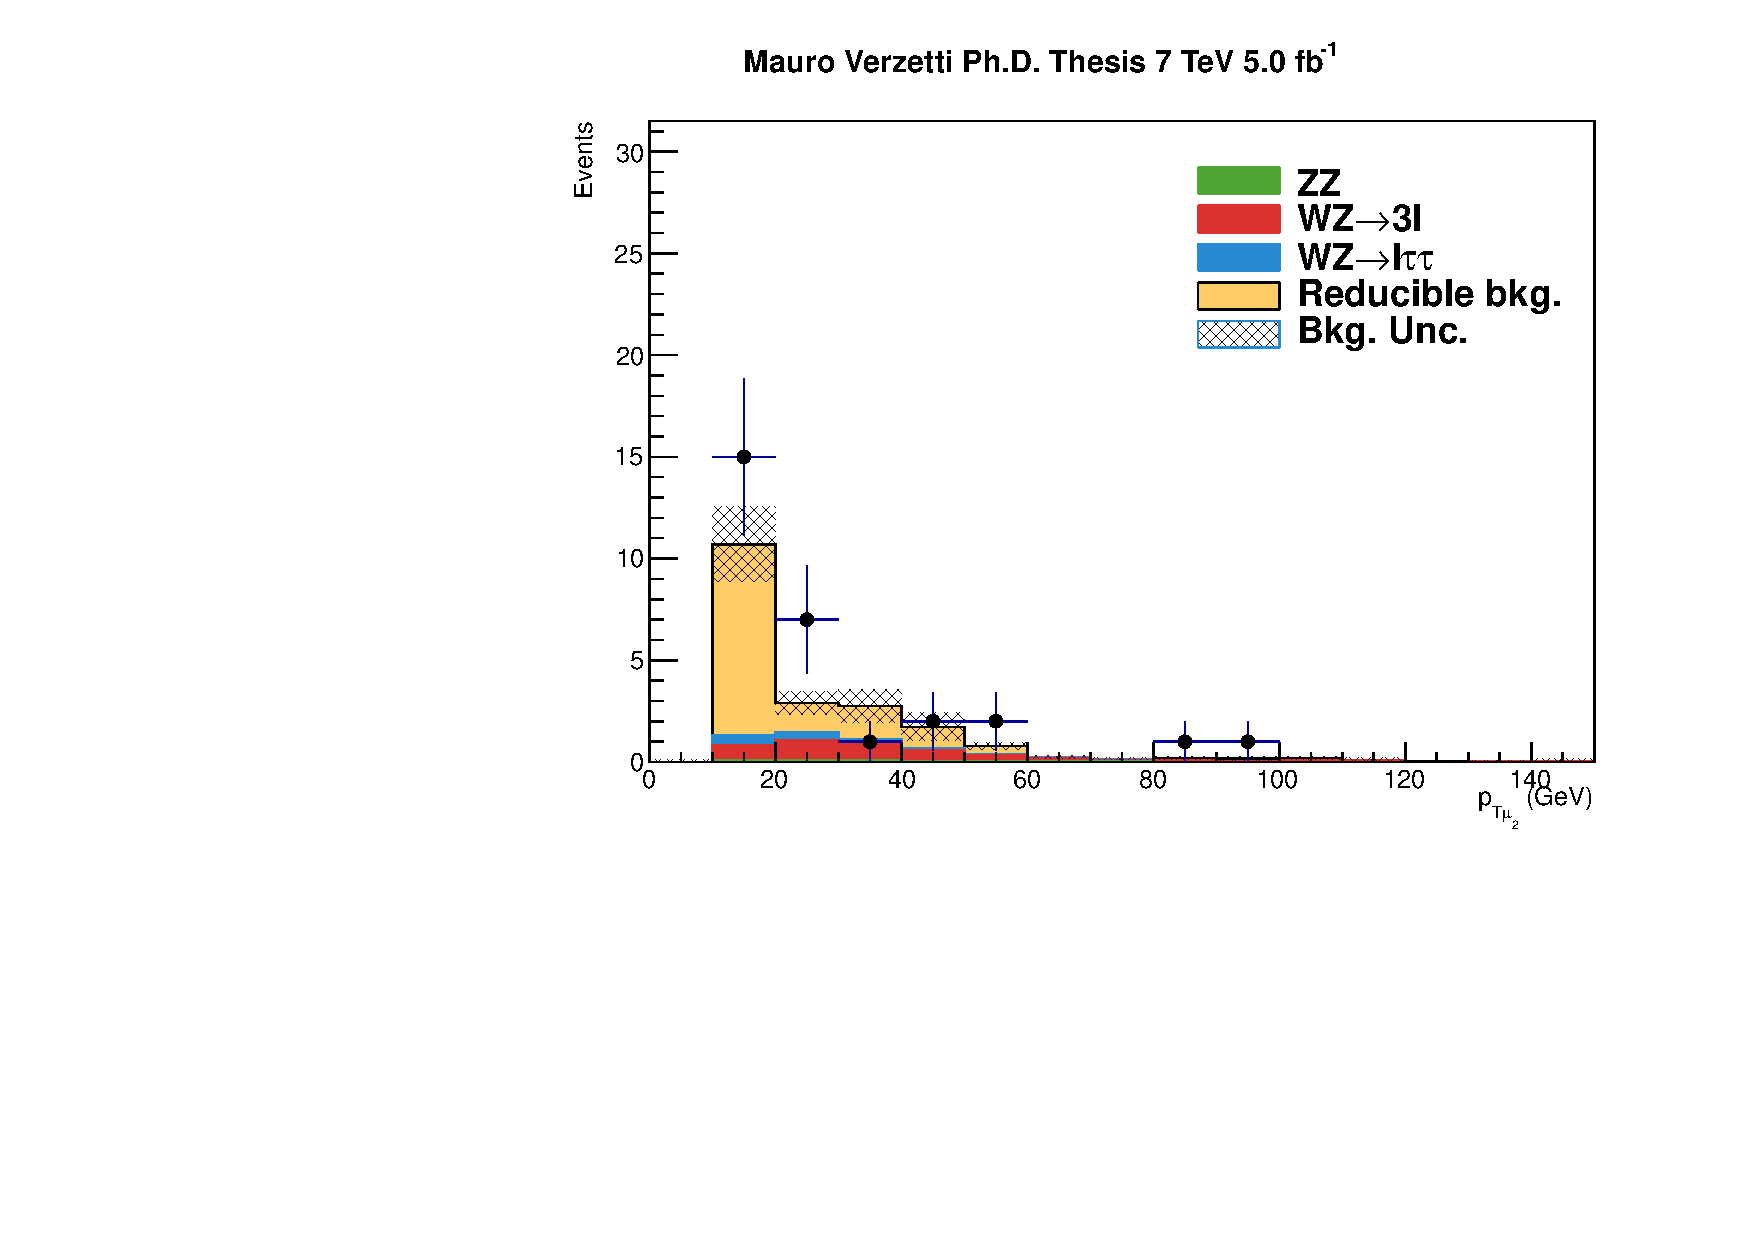
\includegraphics[width=0.49\textwidth]{4_Analisys/pics/7TeV/plots/mmt/f3/Full_charge3/final-f3-m2Pt-Full.pdf}\\
  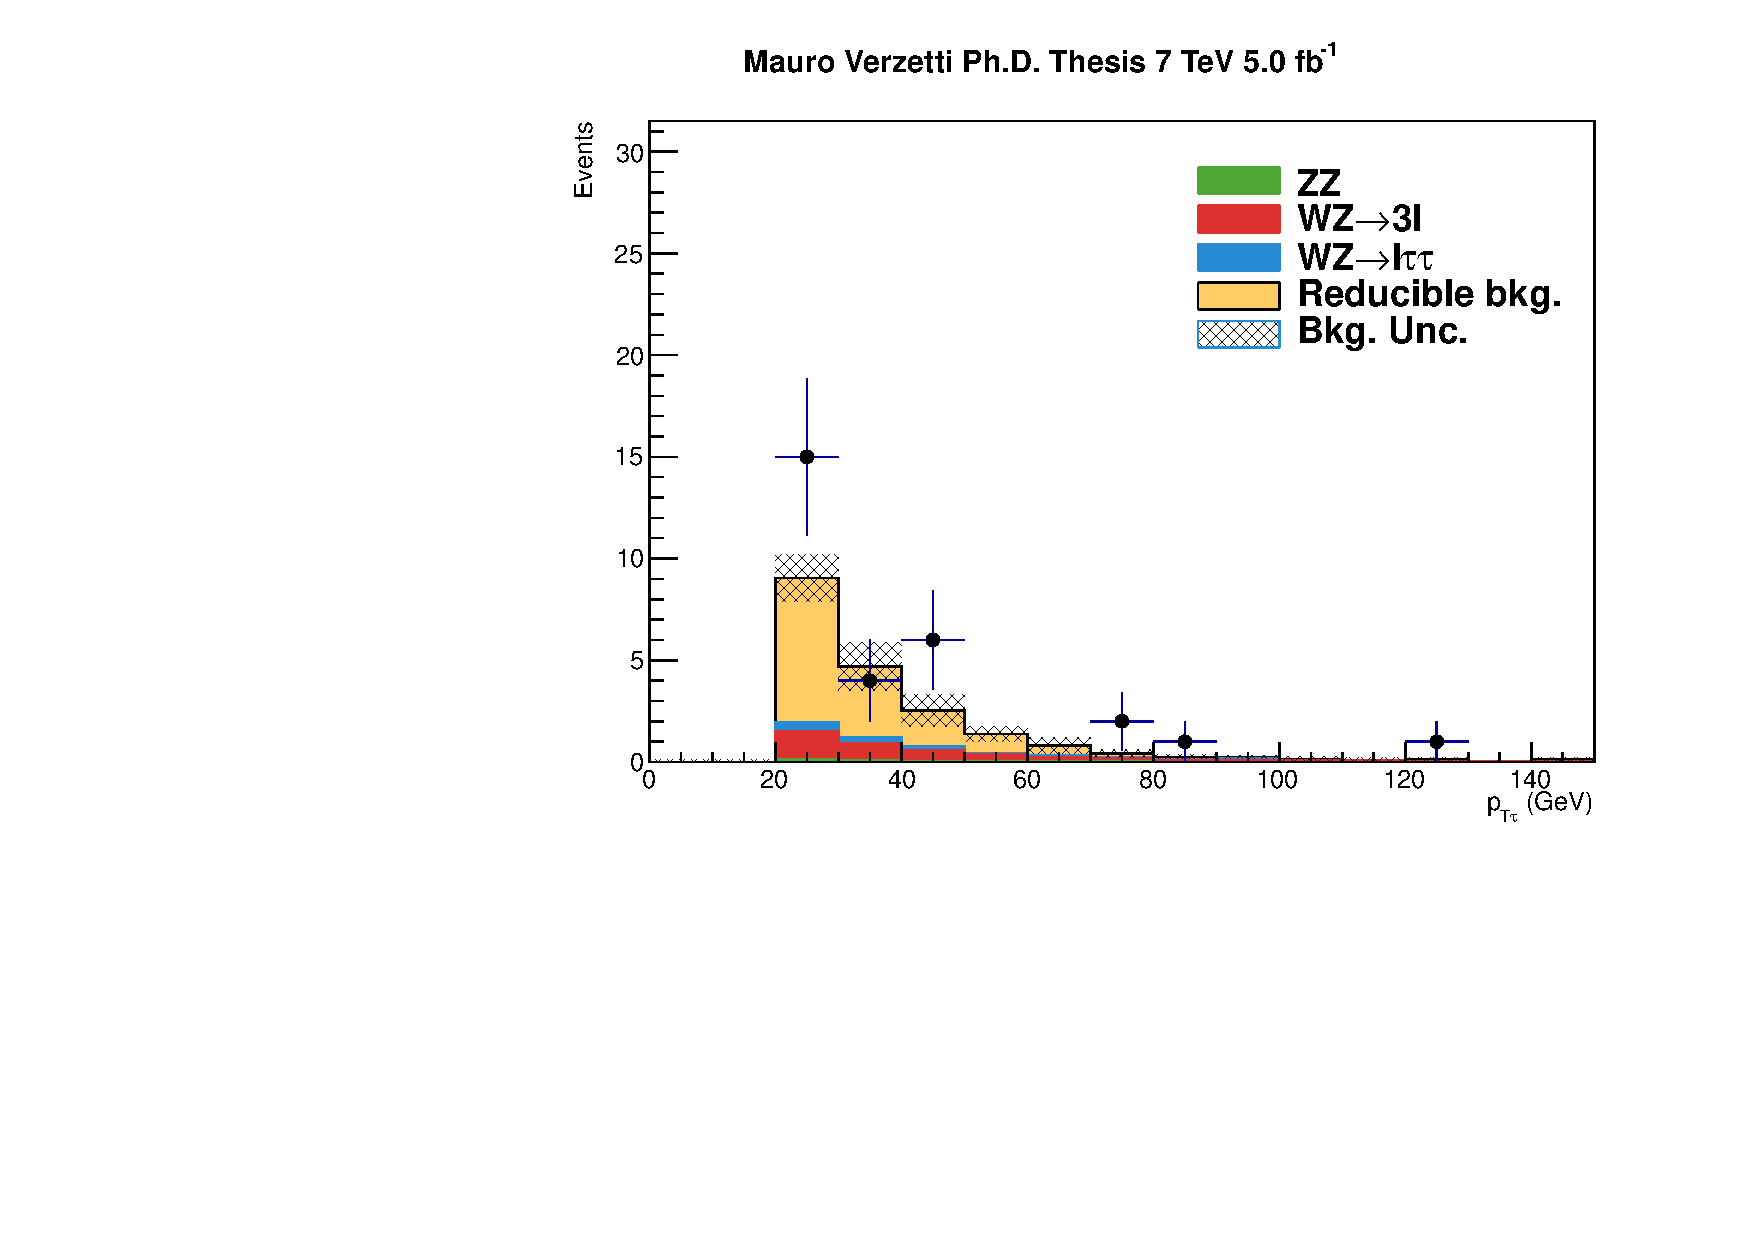
\includegraphics[width=0.49\textwidth]{4_Analisys/pics/7TeV/plots/mmt/f3/Full_charge3/final-f3-tPt-Full.pdf}
  \caption{Comparison of measured and predicted backgrounds in the $\mu\mu\tau_h$ ``fake tau, charge $\pm3$'' control region for 7 TeV data.
  From top left to bottom: mass of the sub-leading muon and the tau system, scalar sum of the leptons \pT ($L_T$), \pT of the leading and sub-leading muon, and \pT of the hadronic tau.
  The reducible background contribution is estimated by the kNN method, in the same manner as in the signal region.
  The shaded band represents the uncertainty on the sum of the background contributions.
  }
  \label{fig:LLT_mmt_f3_charge3_control_7TeV}
\end{center}
\end{figure}

\begin{figure}
\begin{center}
  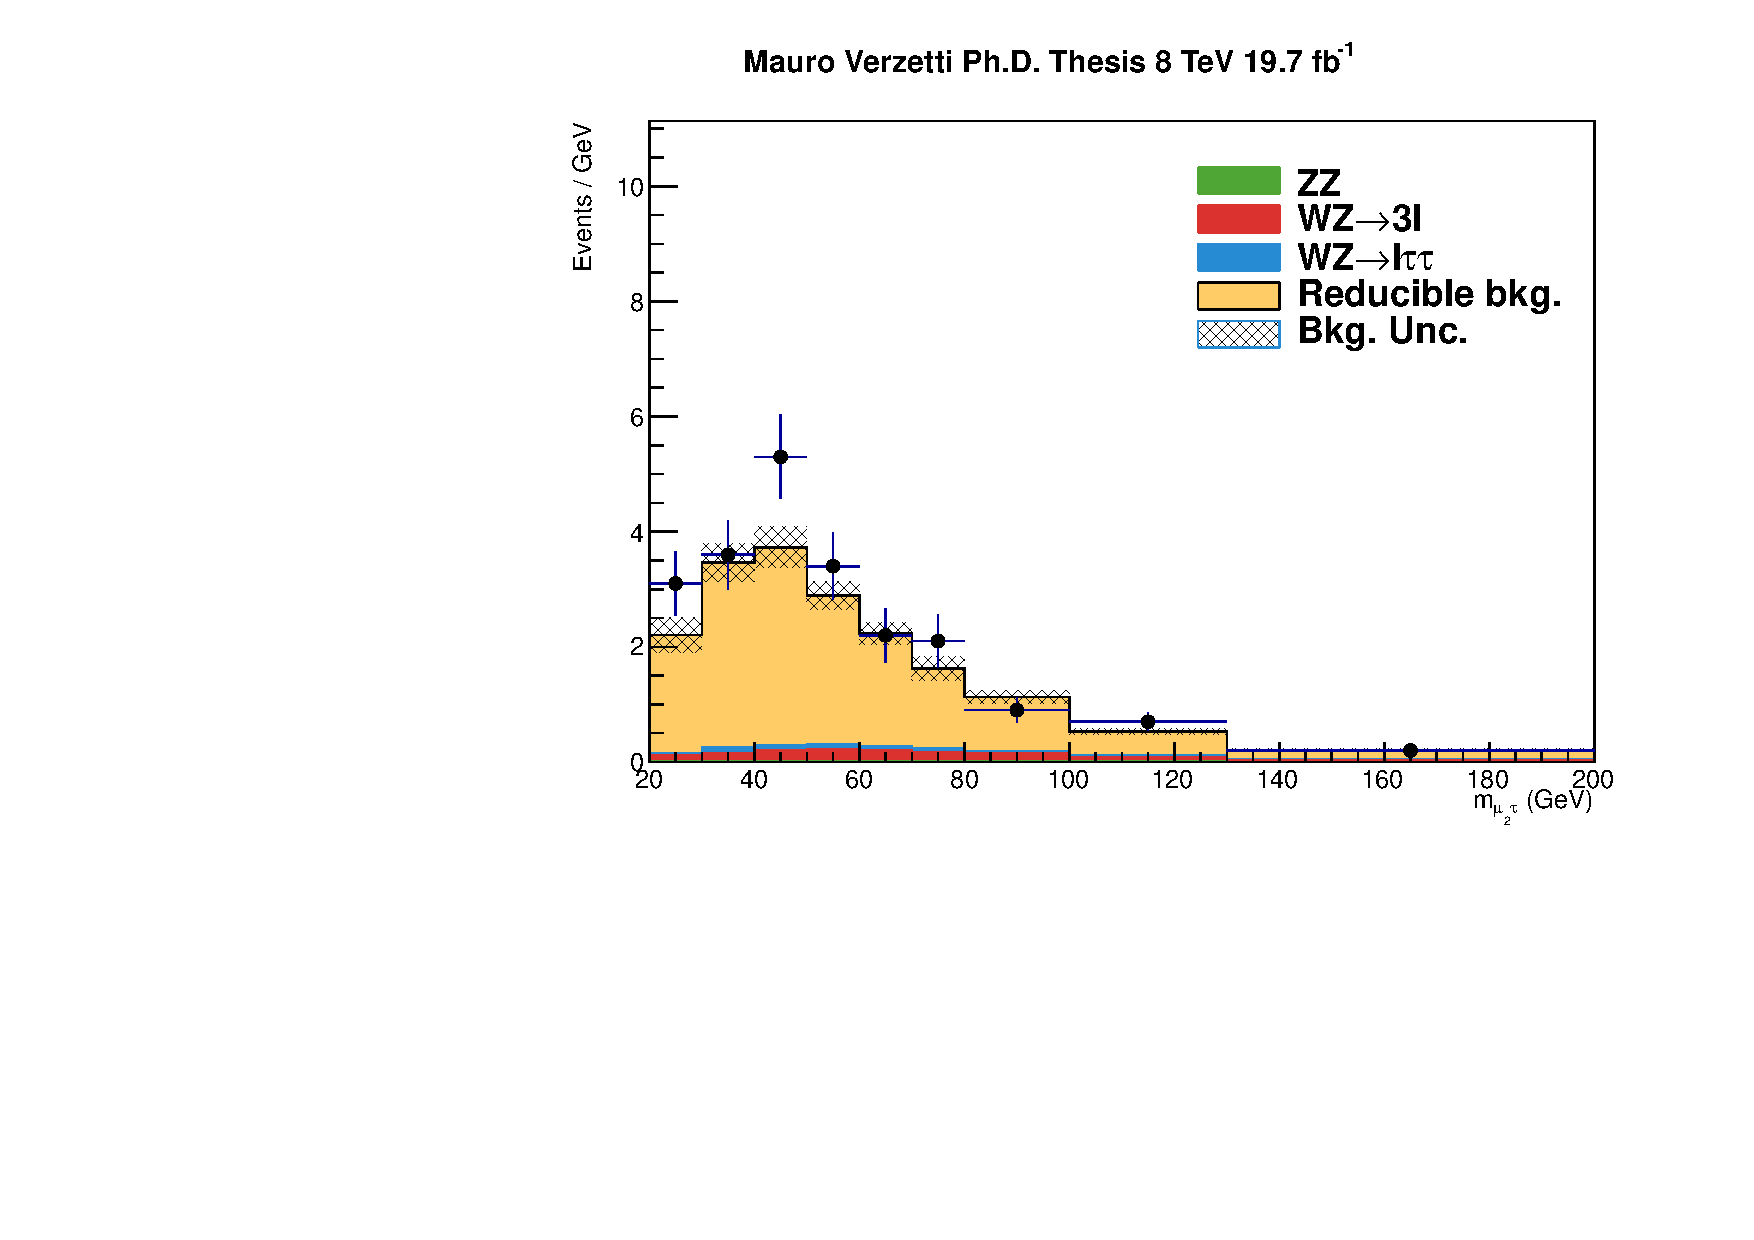
\includegraphics[width=0.49\textwidth]{4_Analisys/pics/8TeV/plots/mmt/f3/Full_charge3/final-f3-subMass-Full.pdf}
  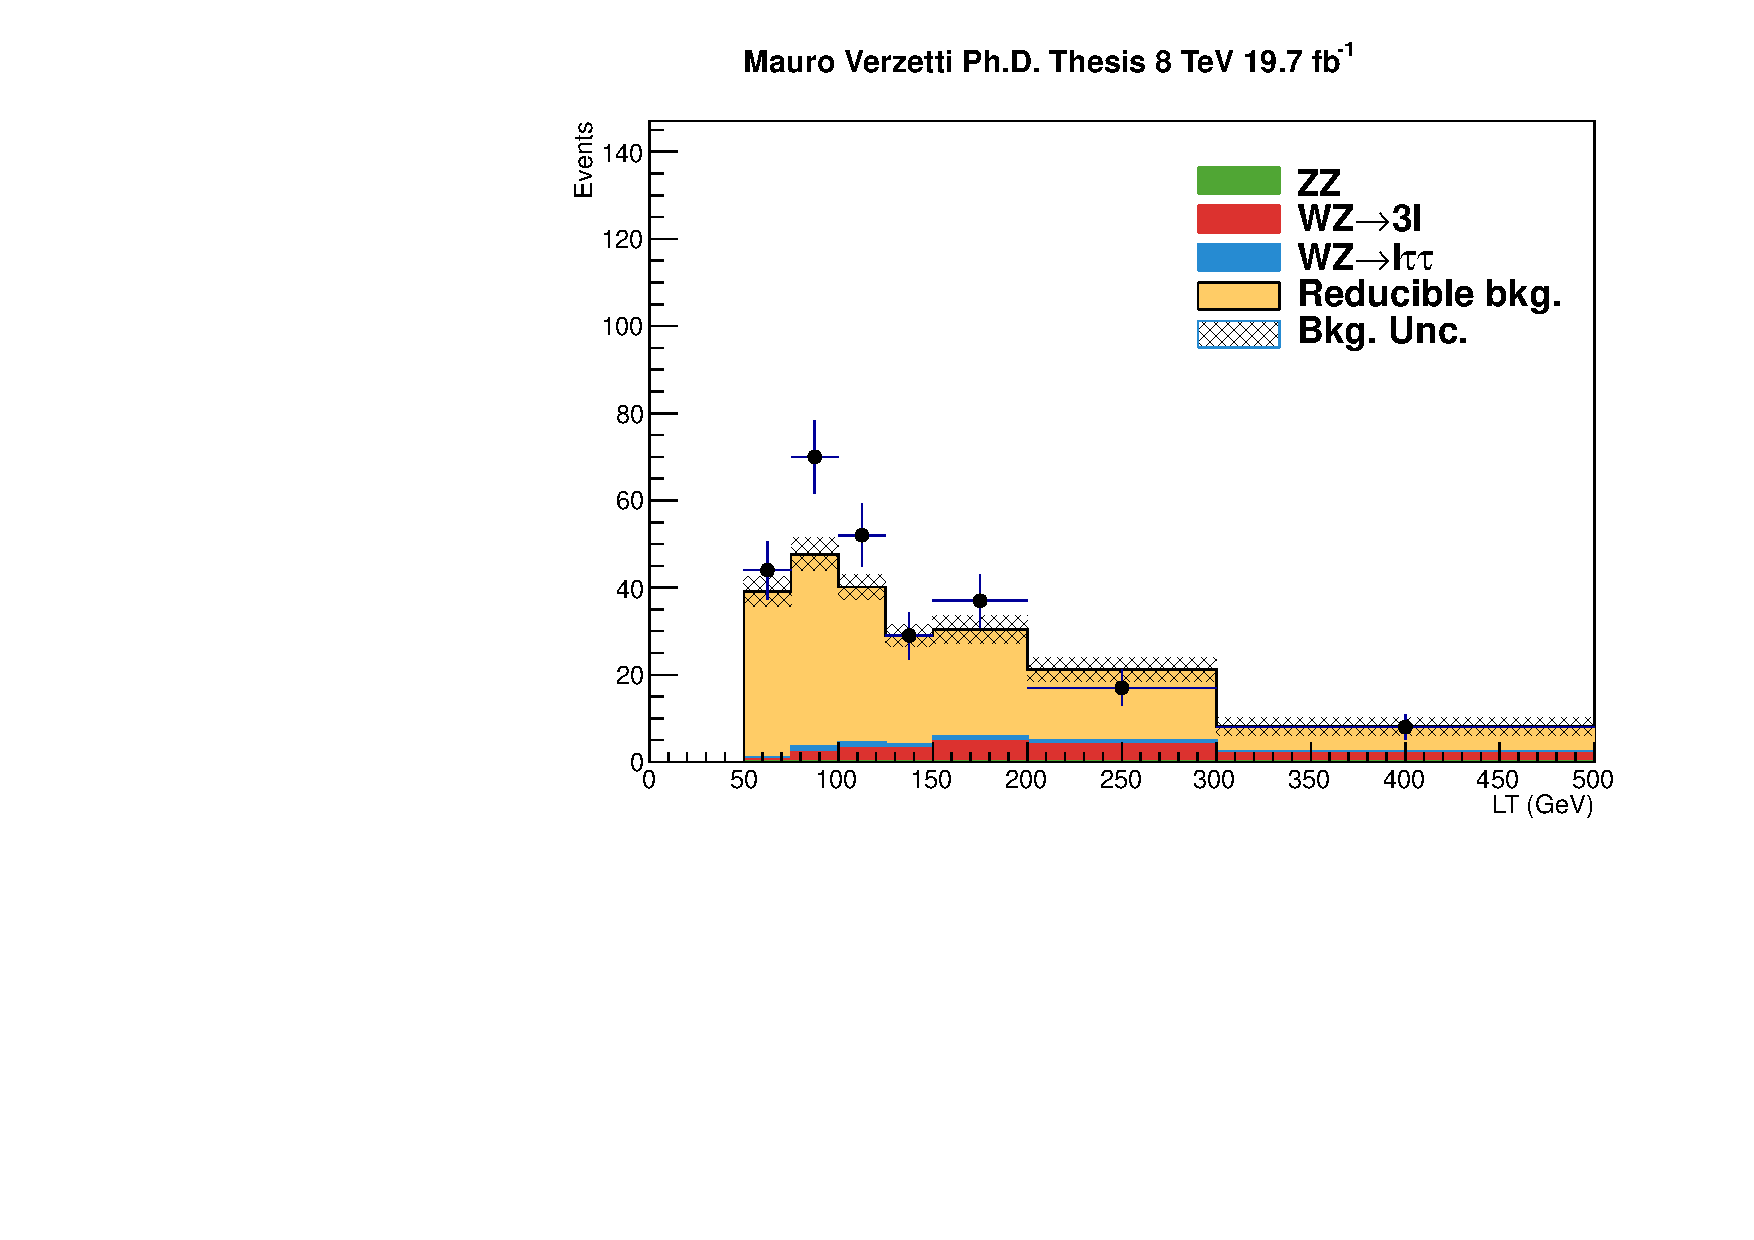
\includegraphics[width=0.49\textwidth]{4_Analisys/pics/8TeV/plots/mmt/f3/final-LT-charge3.pdf}\\
  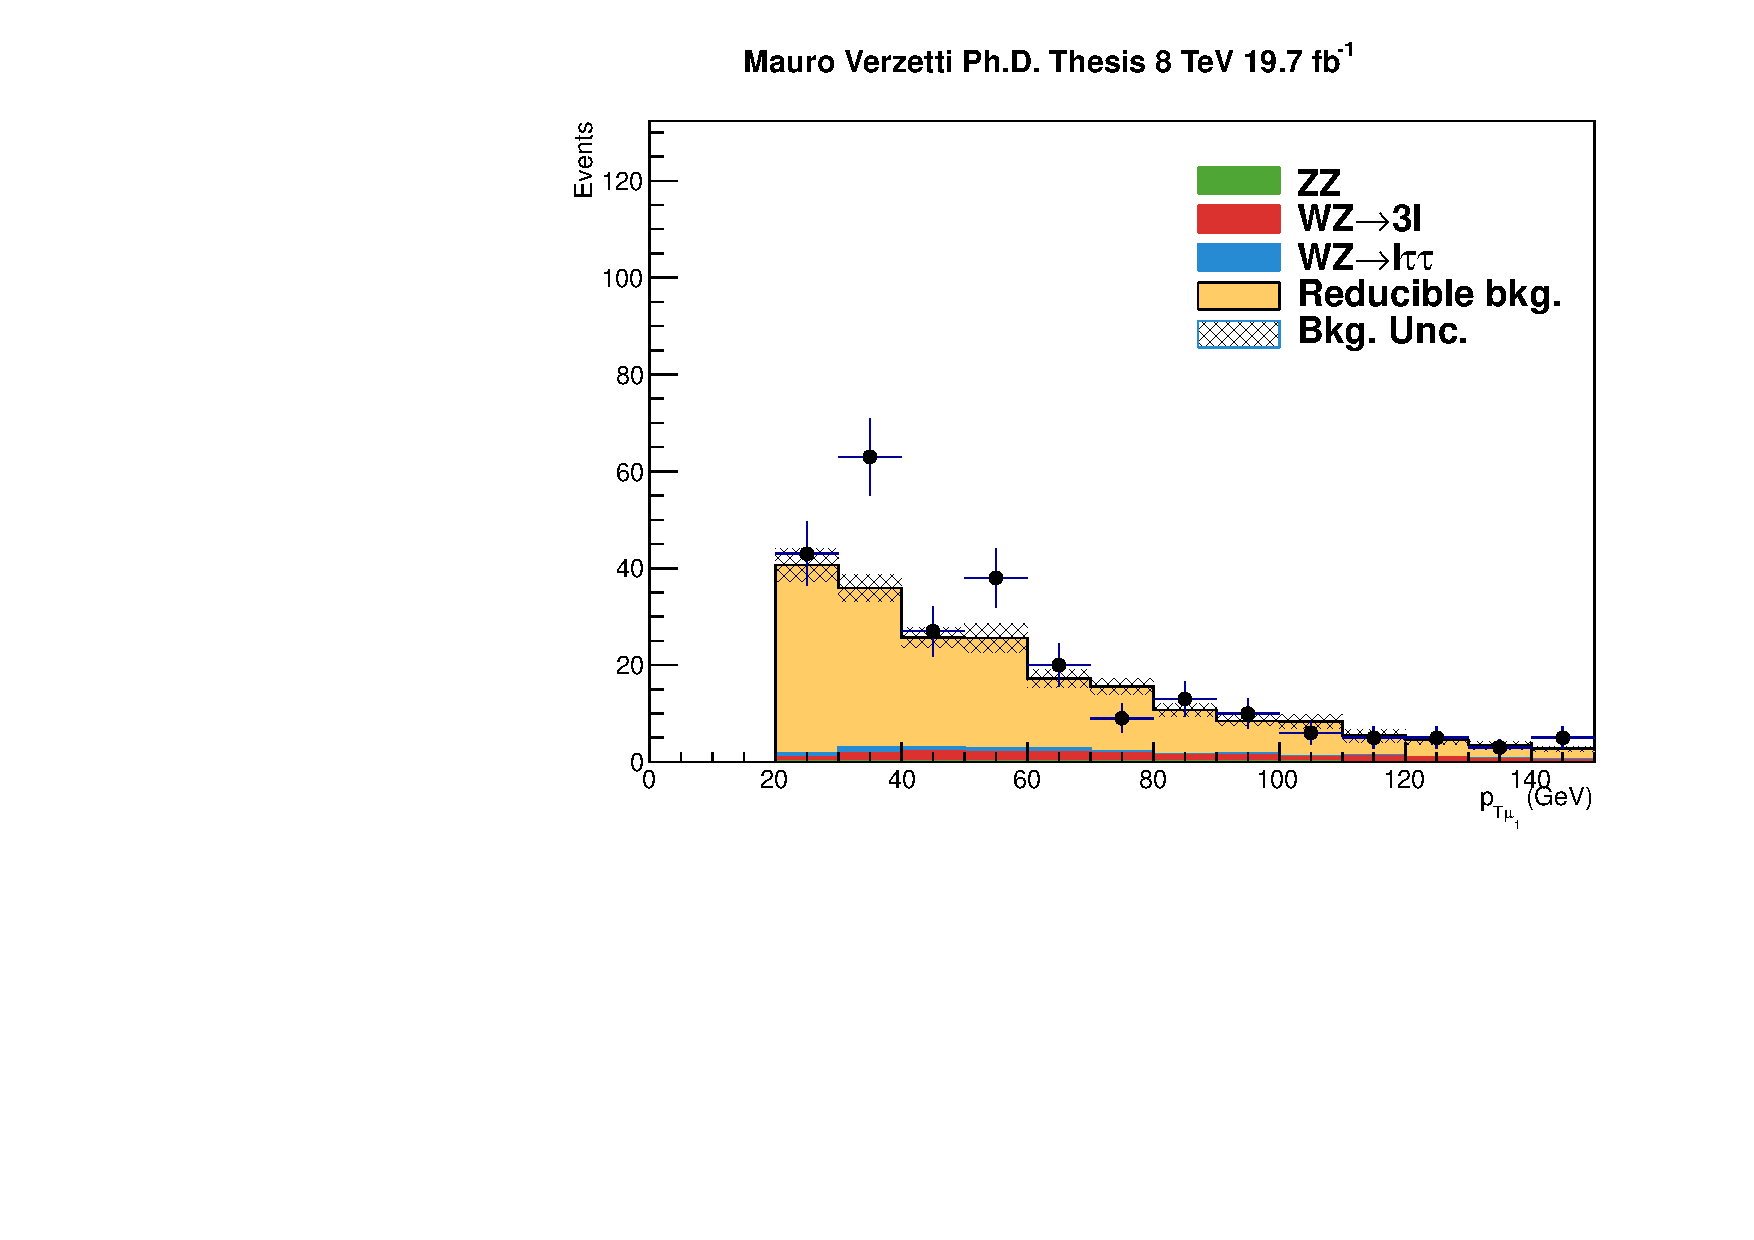
\includegraphics[width=0.49\textwidth]{4_Analisys/pics/8TeV/plots/mmt/f3/Full_charge3/final-f3-m1Pt-Full.pdf}
  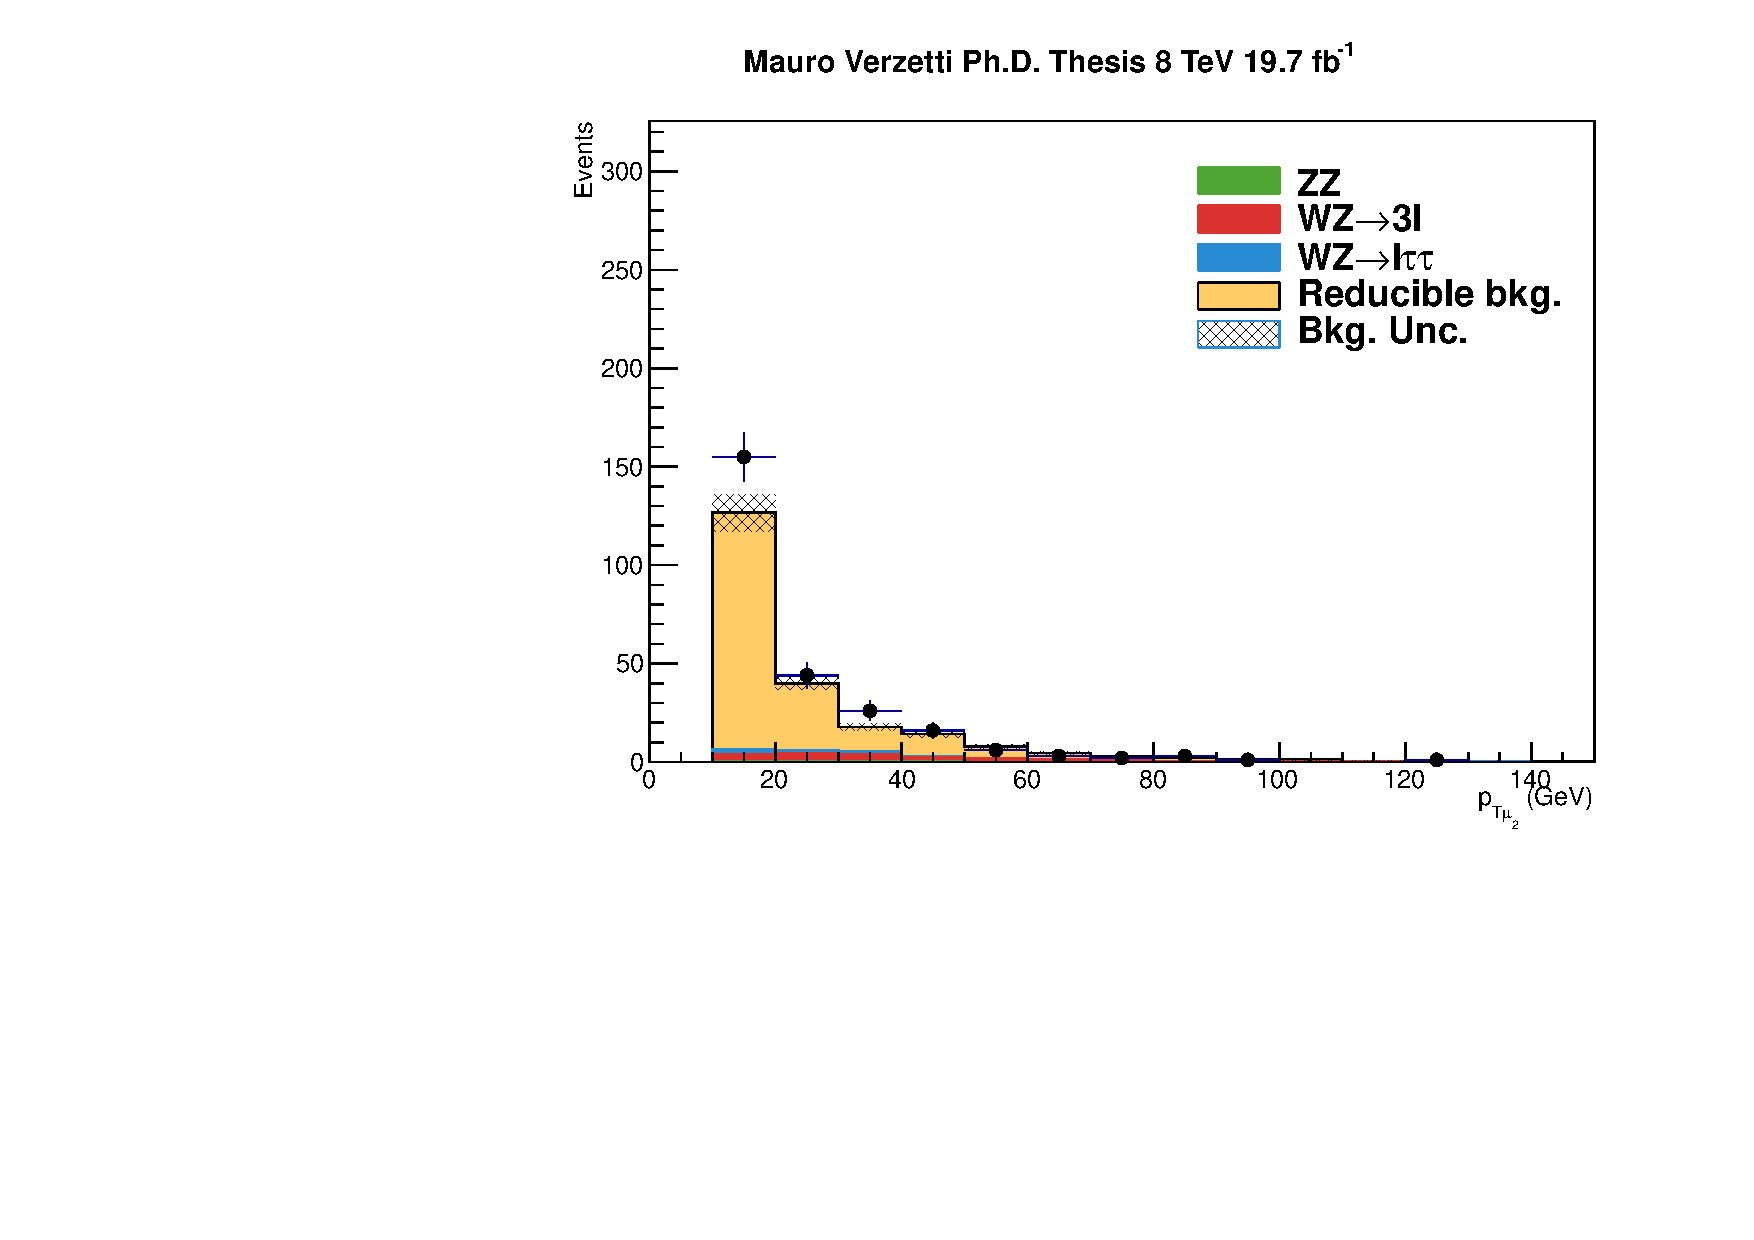
\includegraphics[width=0.49\textwidth]{4_Analisys/pics/8TeV/plots/mmt/f3/Full_charge3/final-f3-m2Pt-Full.pdf}\\
  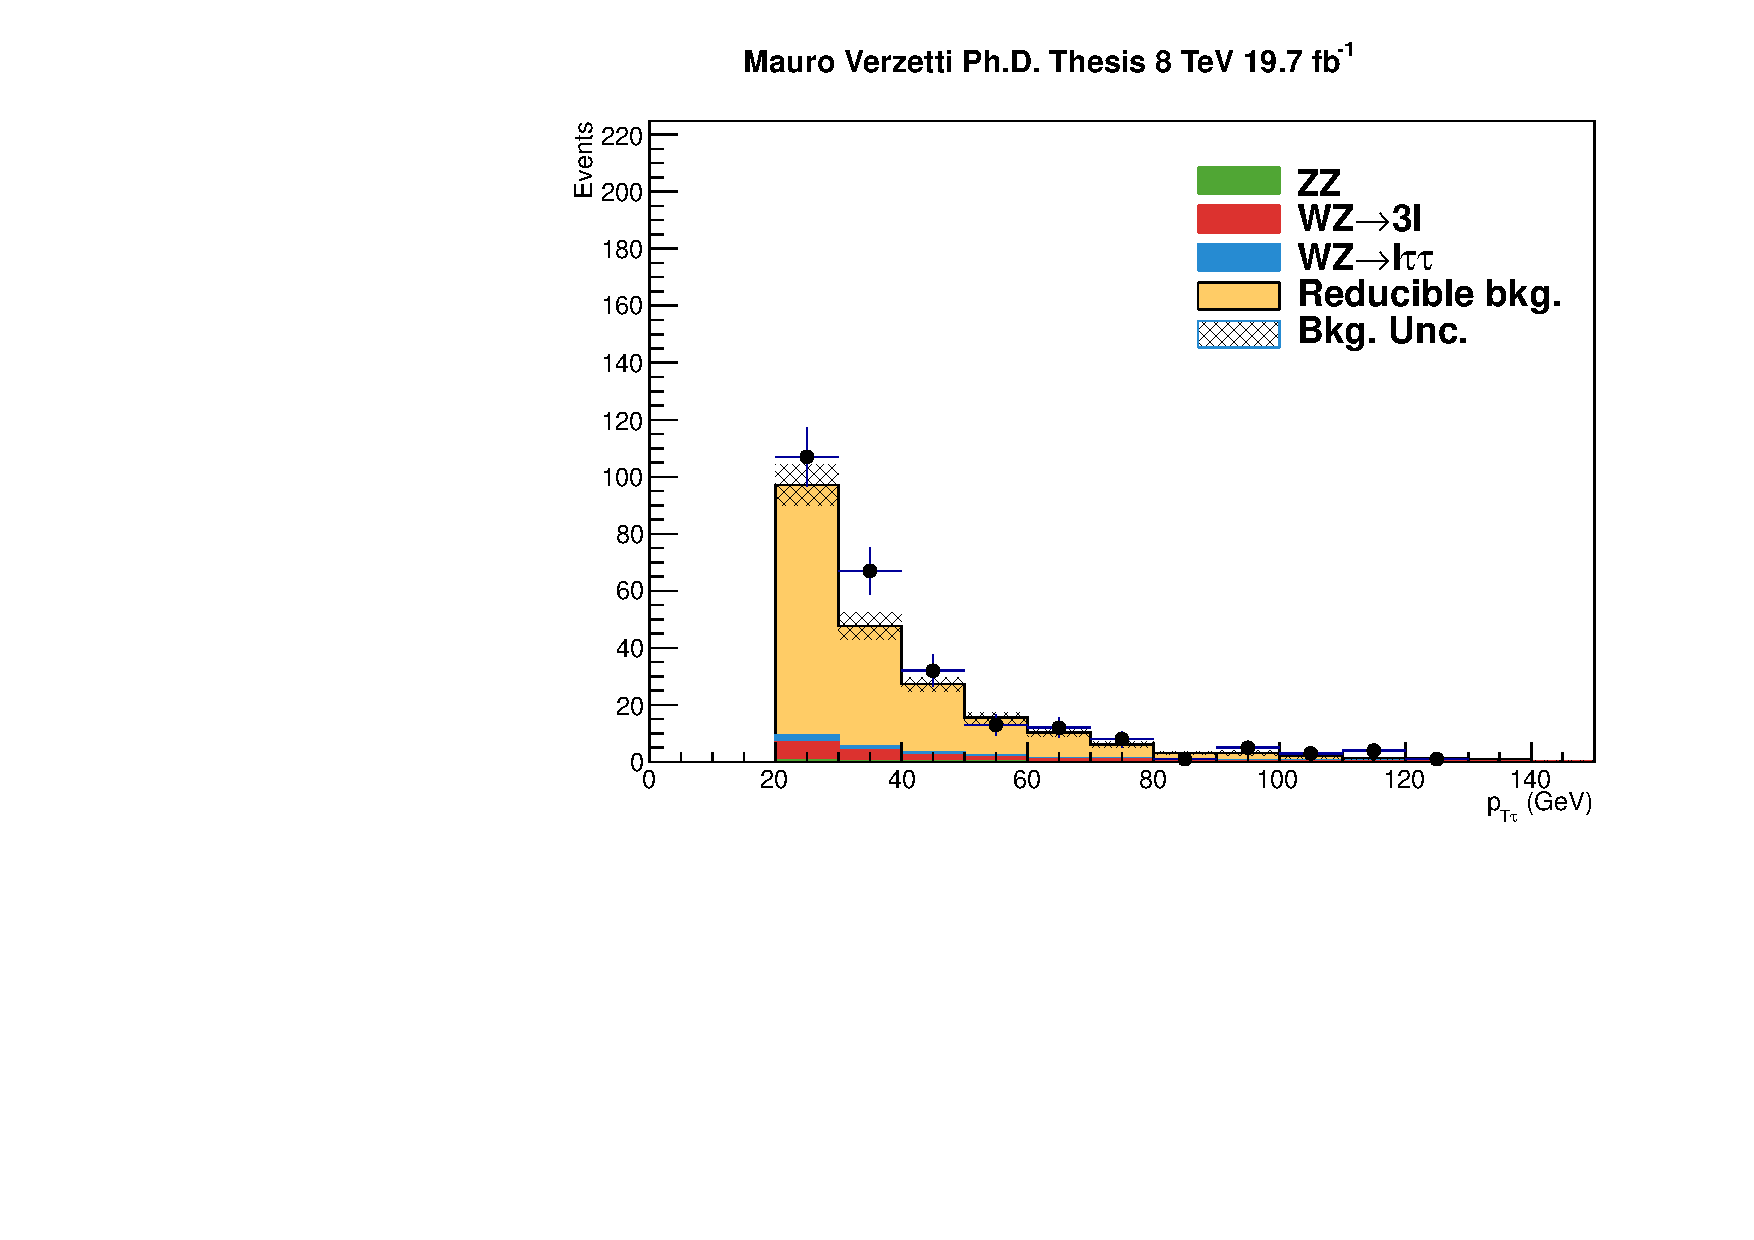
\includegraphics[width=0.49\textwidth]{4_Analisys/pics/8TeV/plots/mmt/f3/Full_charge3/final-f3-tPt-Full.pdf}
  \caption{Comparison of measured and predicted backgrounds in the $\mu\mu\tau_h$ ``fake tau, charge $\pm3$'' control region for 8 TeV data.
  From top left to bottom: mass of the sub-leading muon and the tau system, scalar sum of the leptons \pT ($L_T$), \pT of the leading and sub-leading muon, and \pT of the hadronic tau.
  The reducible background contribution is estimated by the kNN method, in the same manner as in the signal region.
  The shaded band represents the uncertainty on the sum of the background contributions.
  }
  \label{fig:LLT_mmt_f3_charge3_control_8TeV}
\end{center}
\end{figure}

\begin{figure}
\begin{center}
  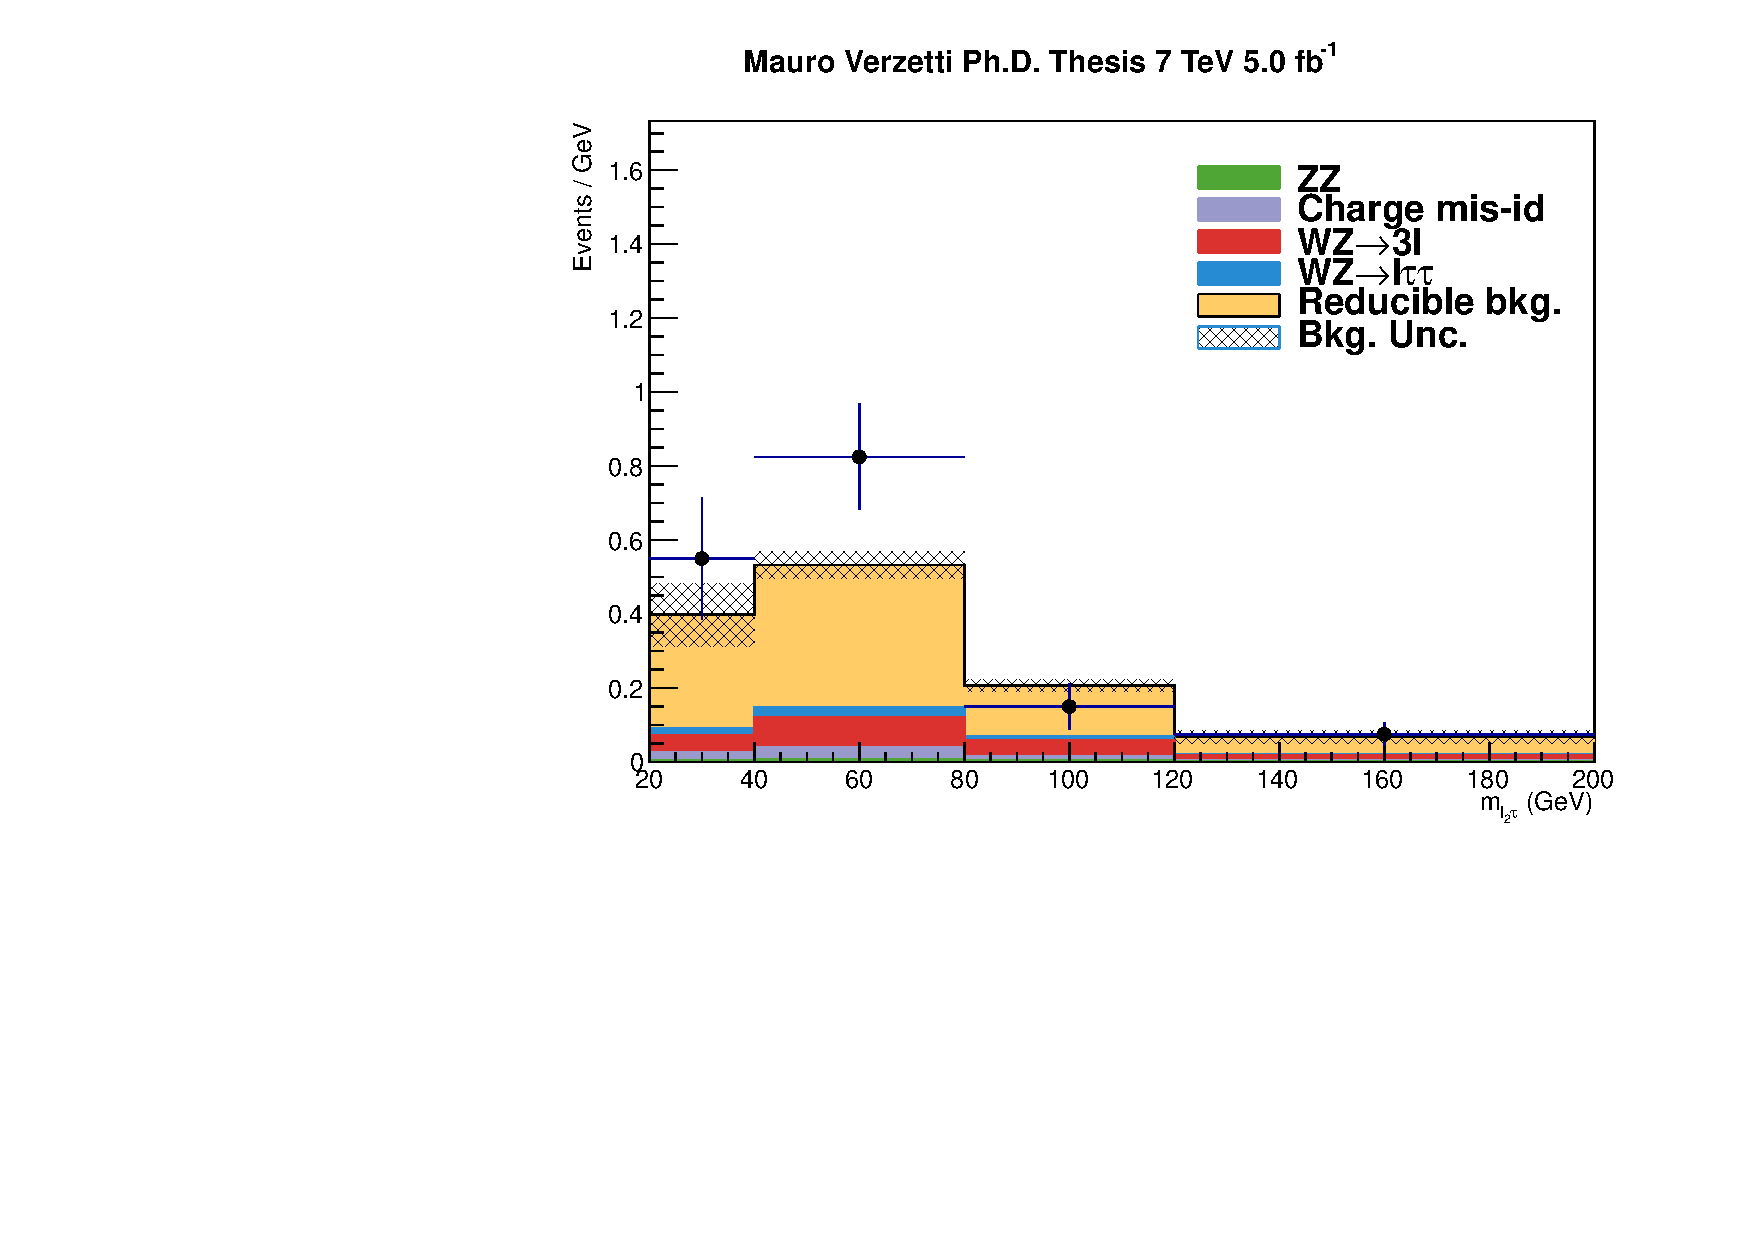
\includegraphics[width=0.49\textwidth]{4_Analisys/pics/7TeV/plots/emt/f3/Full_charge3/final-f3-subMass-Full.pdf}
  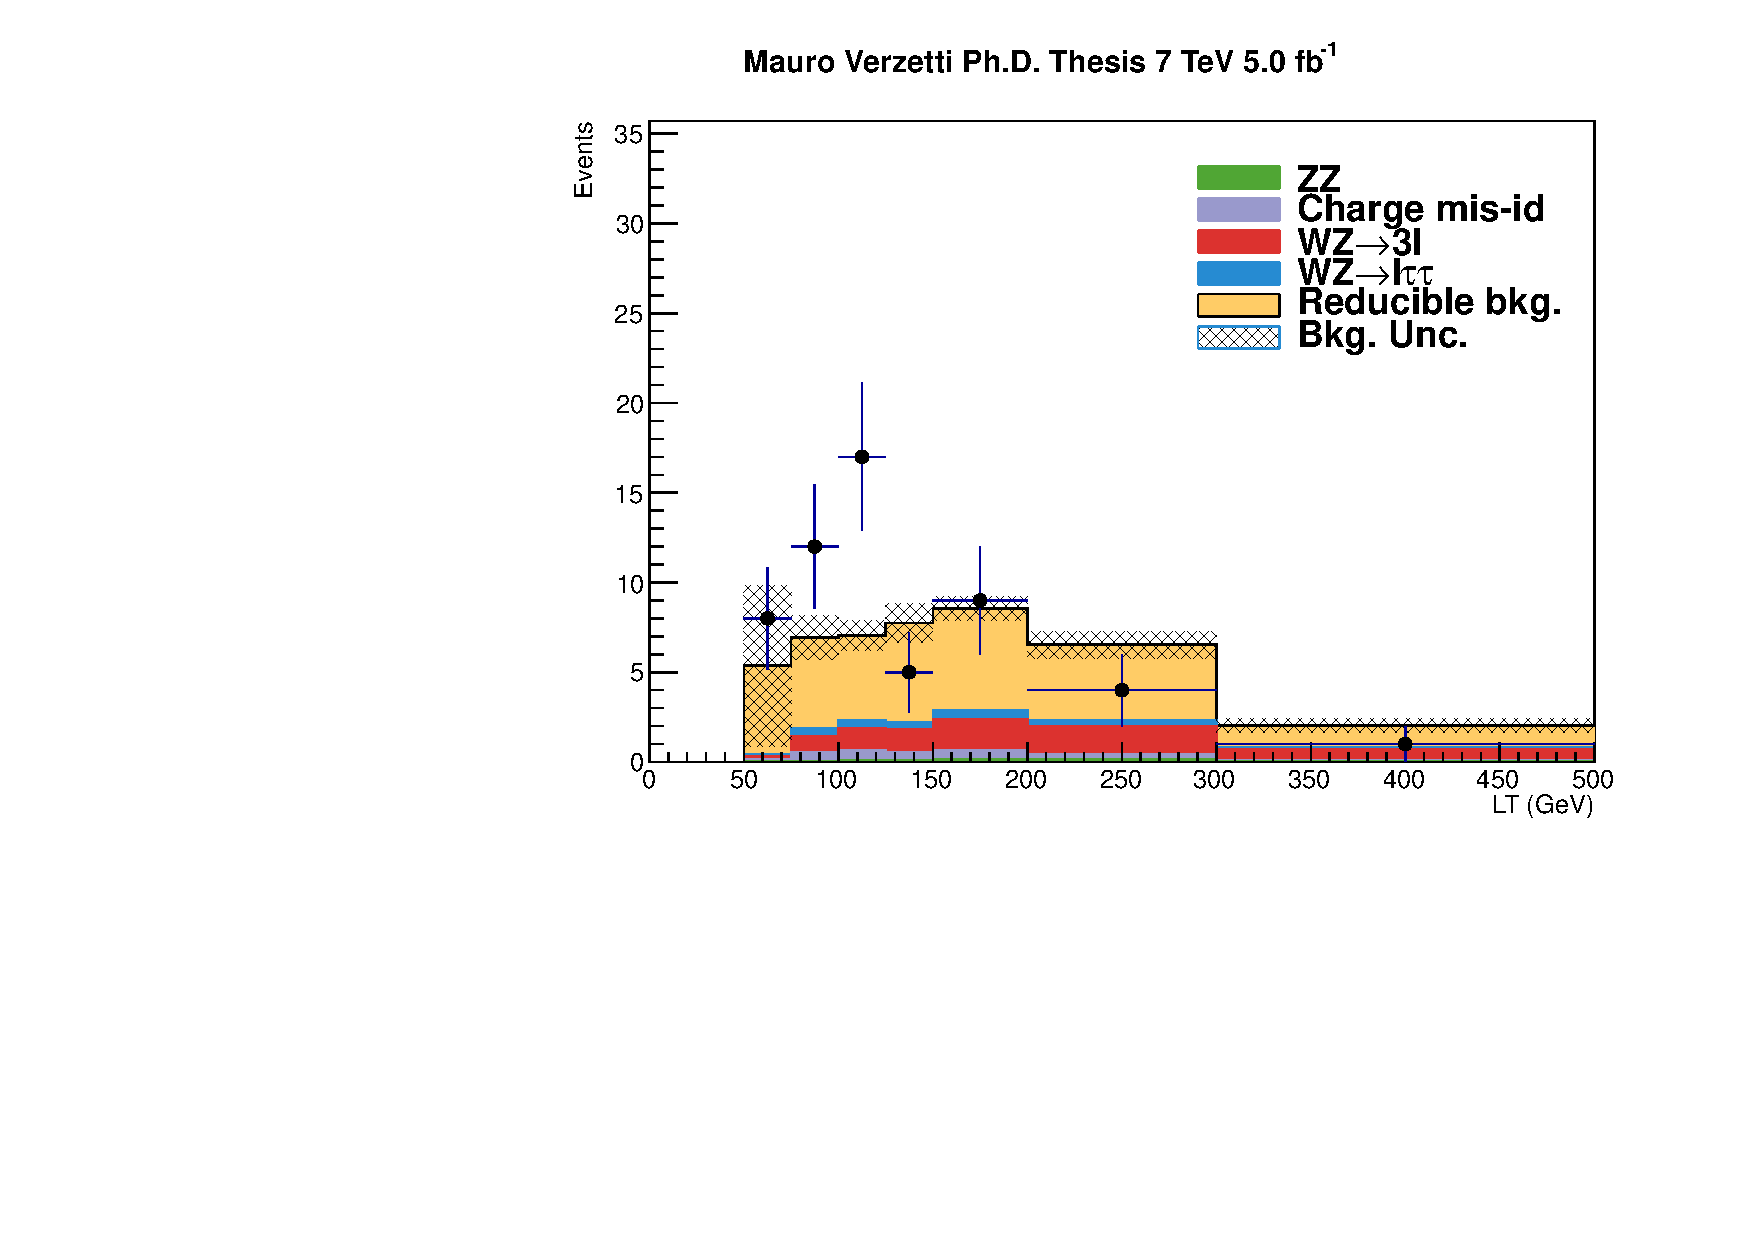
\includegraphics[width=0.49\textwidth]{4_Analisys/pics/7TeV/plots/emt/f3/final-f3-LT-charge3.pdf}\\
  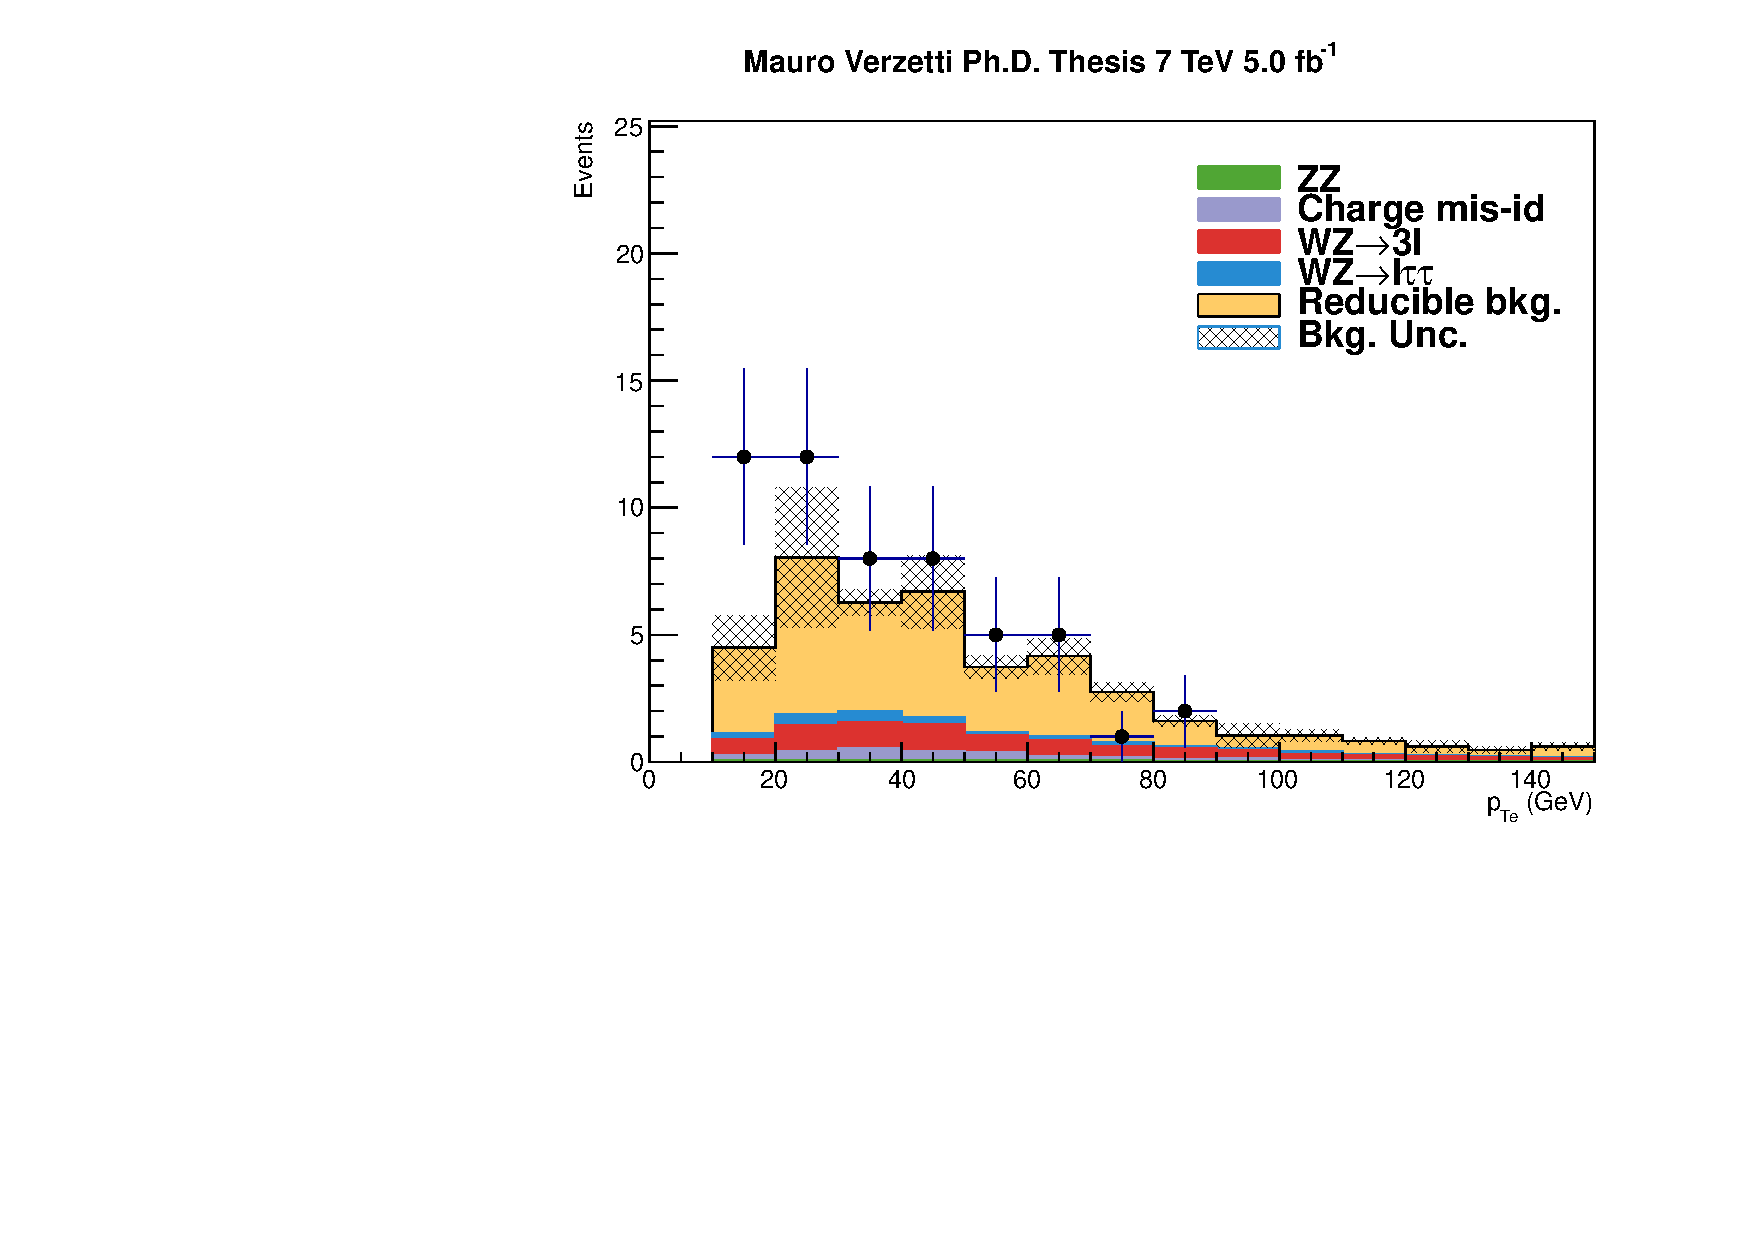
\includegraphics[width=0.49\textwidth]{4_Analisys/pics/7TeV/plots/emt/f3/Full_charge3/final-f3-ePt-Full.pdf}
  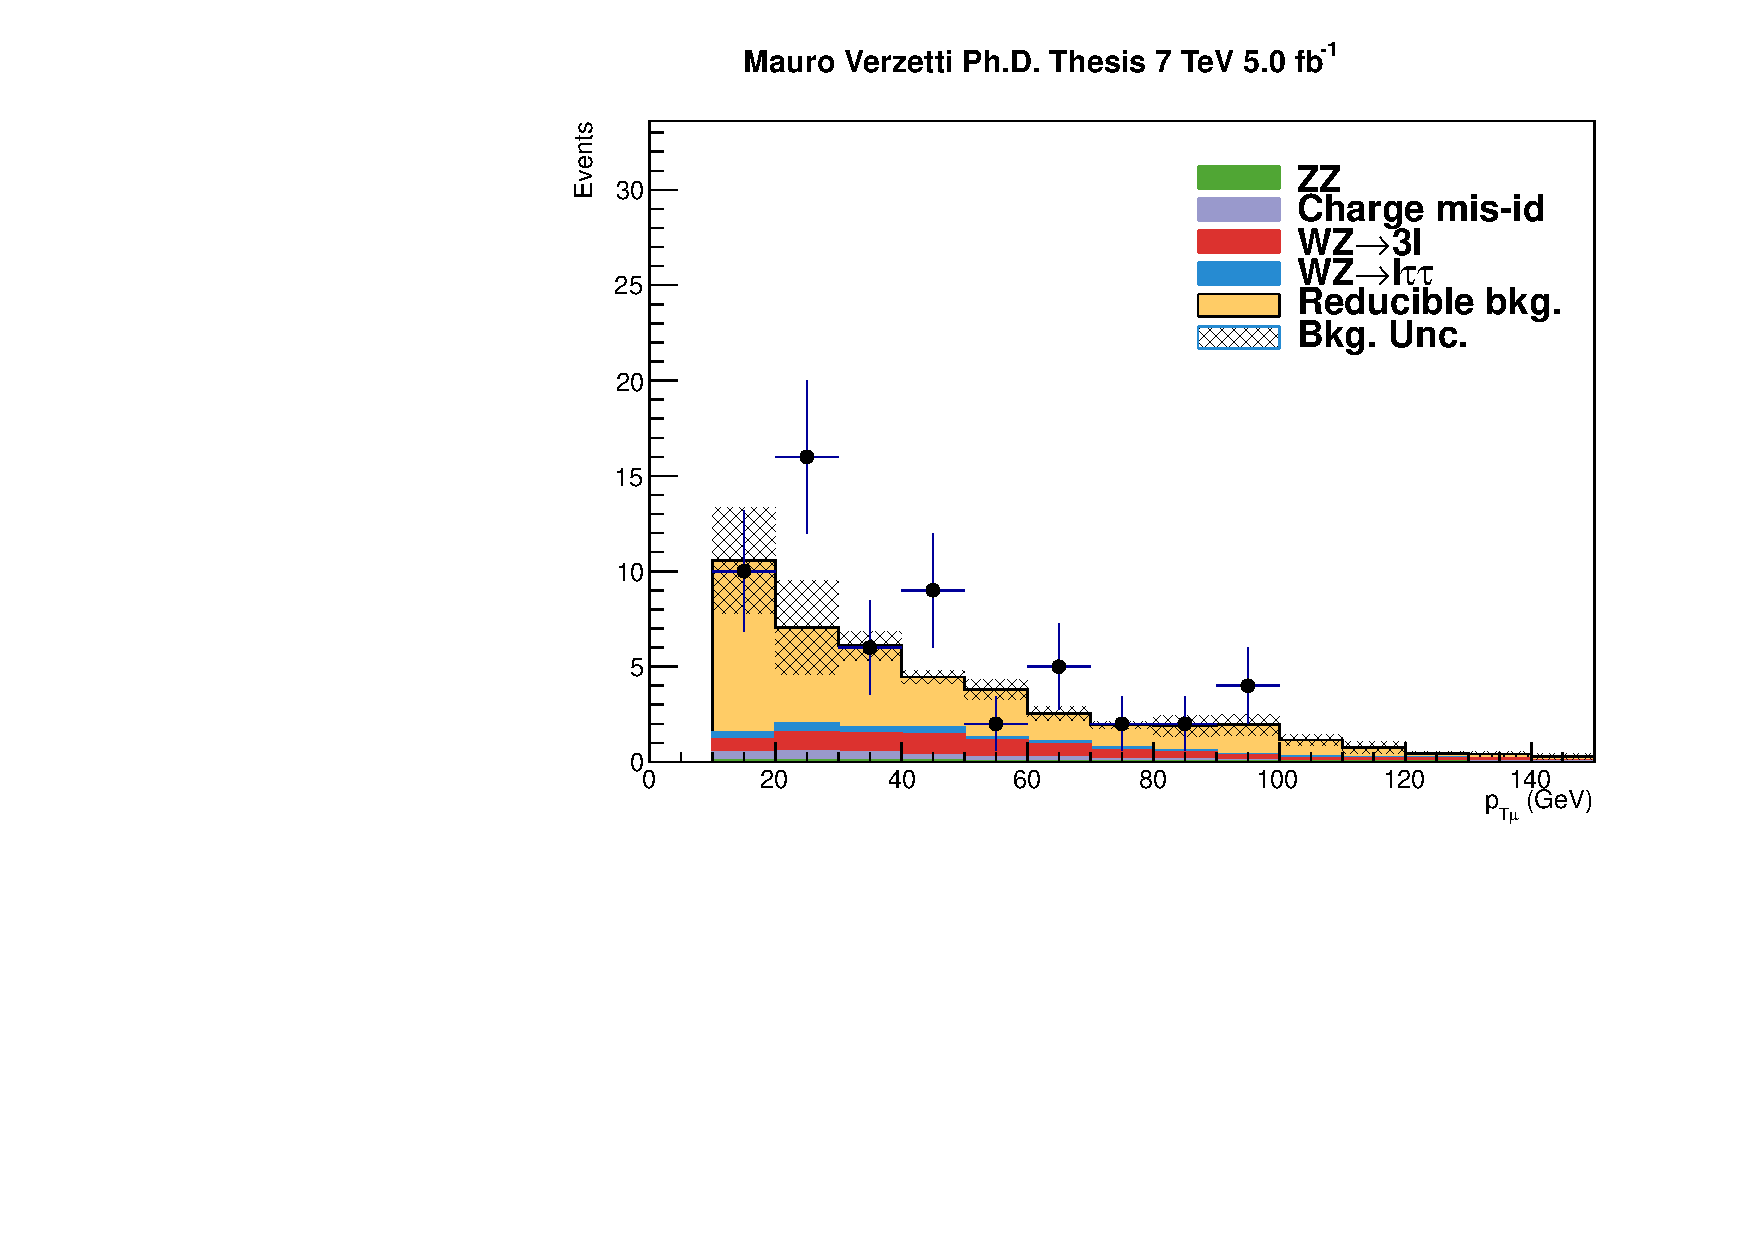
\includegraphics[width=0.49\textwidth]{4_Analisys/pics/7TeV/plots/emt/f3/Full_charge3/final-f3-mPt-Full.pdf}\\
  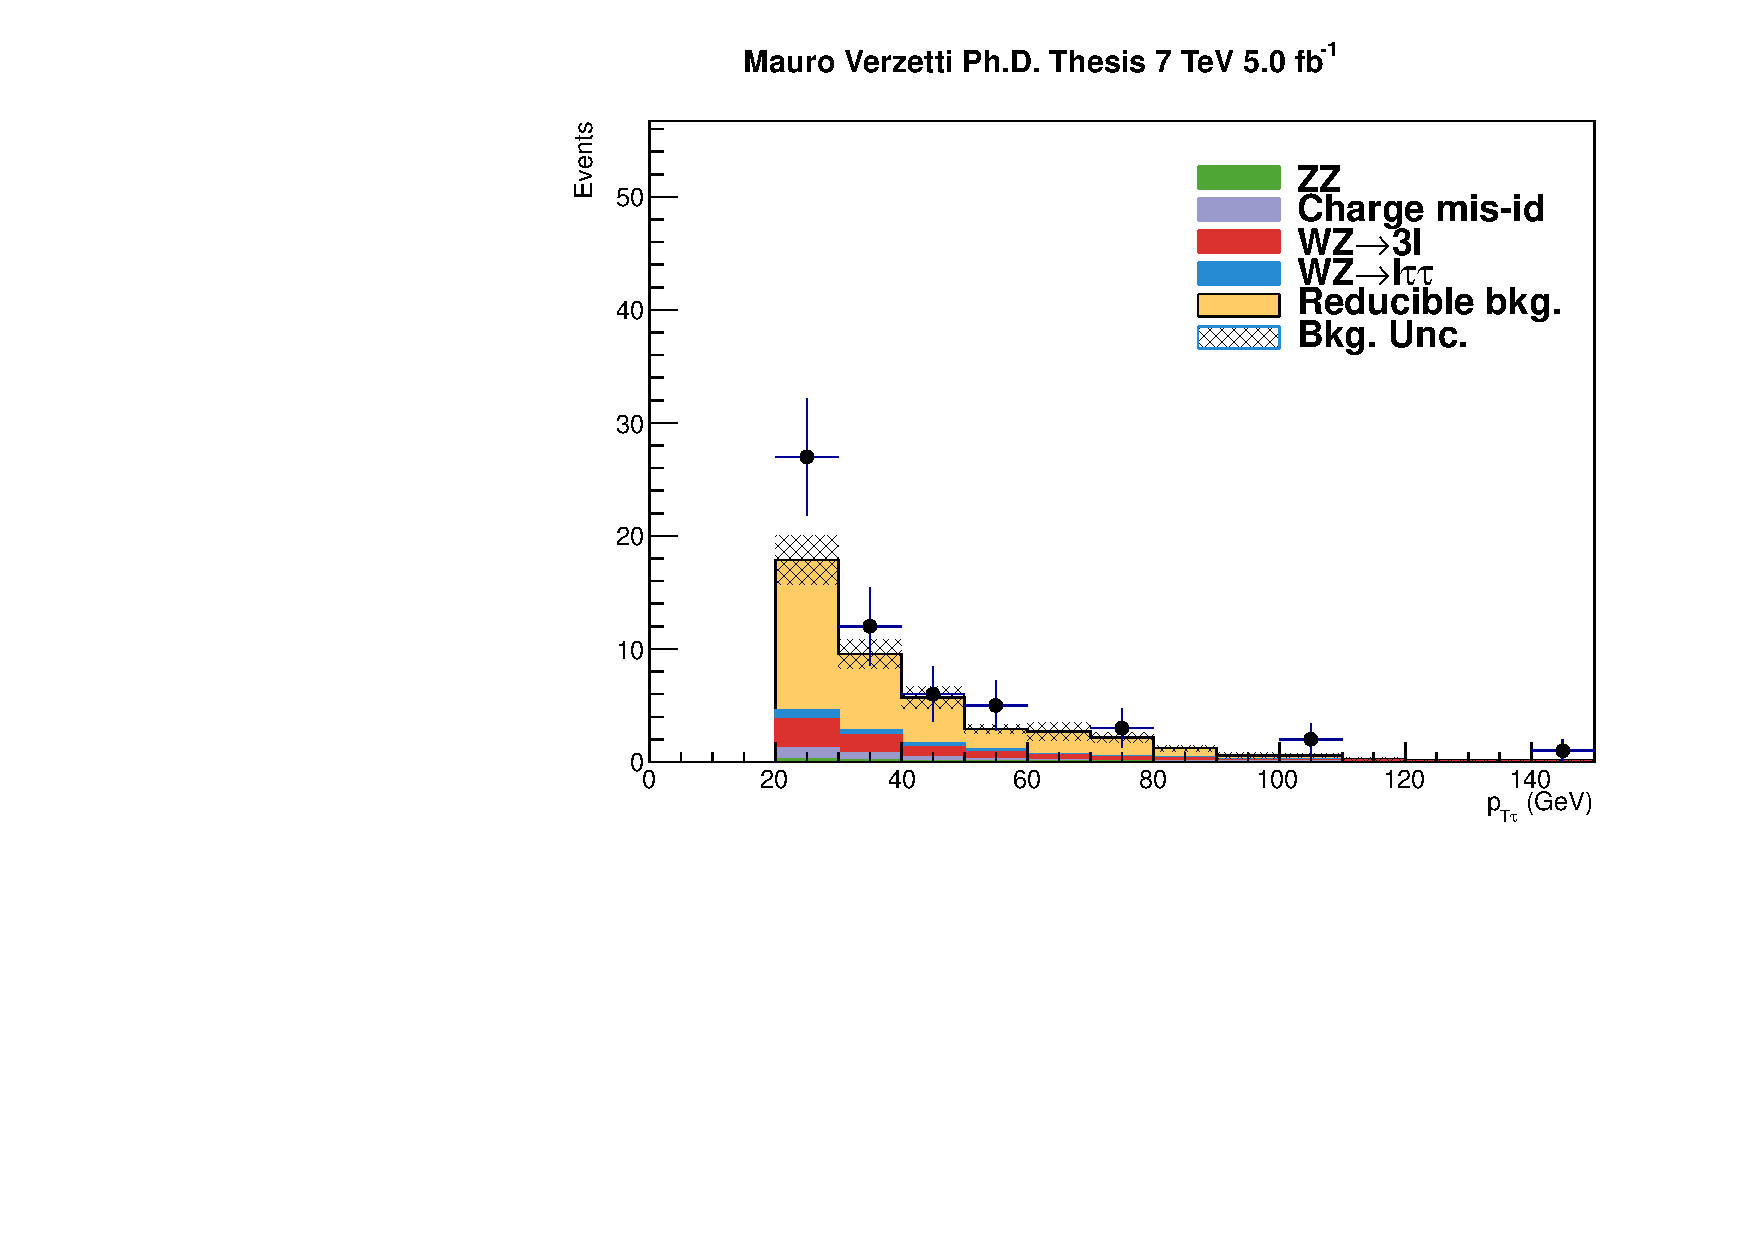
\includegraphics[width=0.49\textwidth]{4_Analisys/pics/7TeV/plots/emt/f3/Full_charge3/final-f3-tPt-Full.pdf}
  \caption{Comparison of measured and predicted backgrounds in the $e\mu\tau_h$ ``fake tau, charge $\pm3$'' control region for 7 TeV data.
  From top left to bottom: mass of the sub-leading lepton and the tau system, scalar sum of the leptons \pT ($L_T$), \pT of the electron, muon, and hadronic tau.
  The reducible background contribution is estimated by the kNN method, in the same manner as in the signal region.
  The shaded band represents the uncertainty on the sum of the background contributions.
  }
  \label{fig:LLT_emt_f3_charge3_control_7TeV}
\end{center}
\end{figure}

\begin{figure}
\begin{center}
  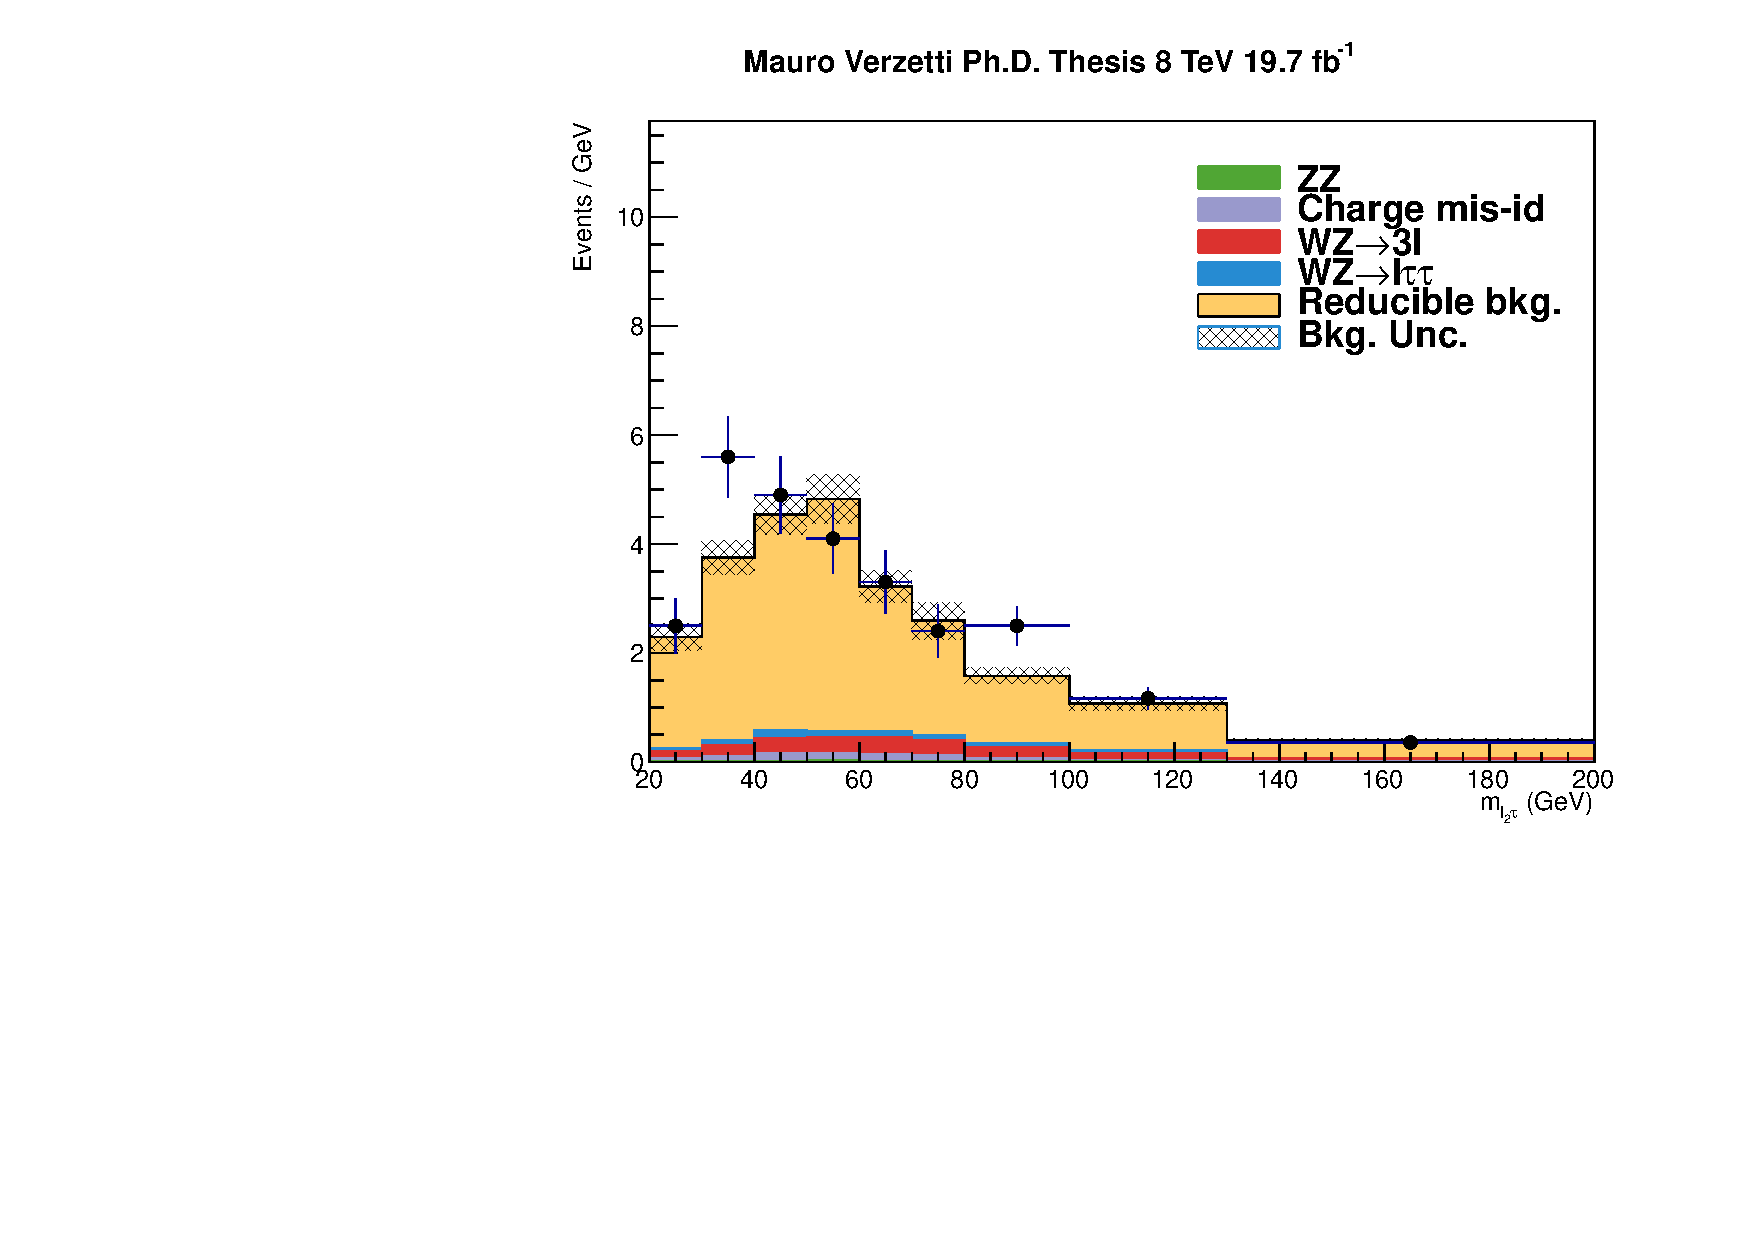
\includegraphics[width=0.49\textwidth]{4_Analisys/pics/8TeV/plots/emt/f3/Full_charge3/final-f3-subMass-Full.pdf}
  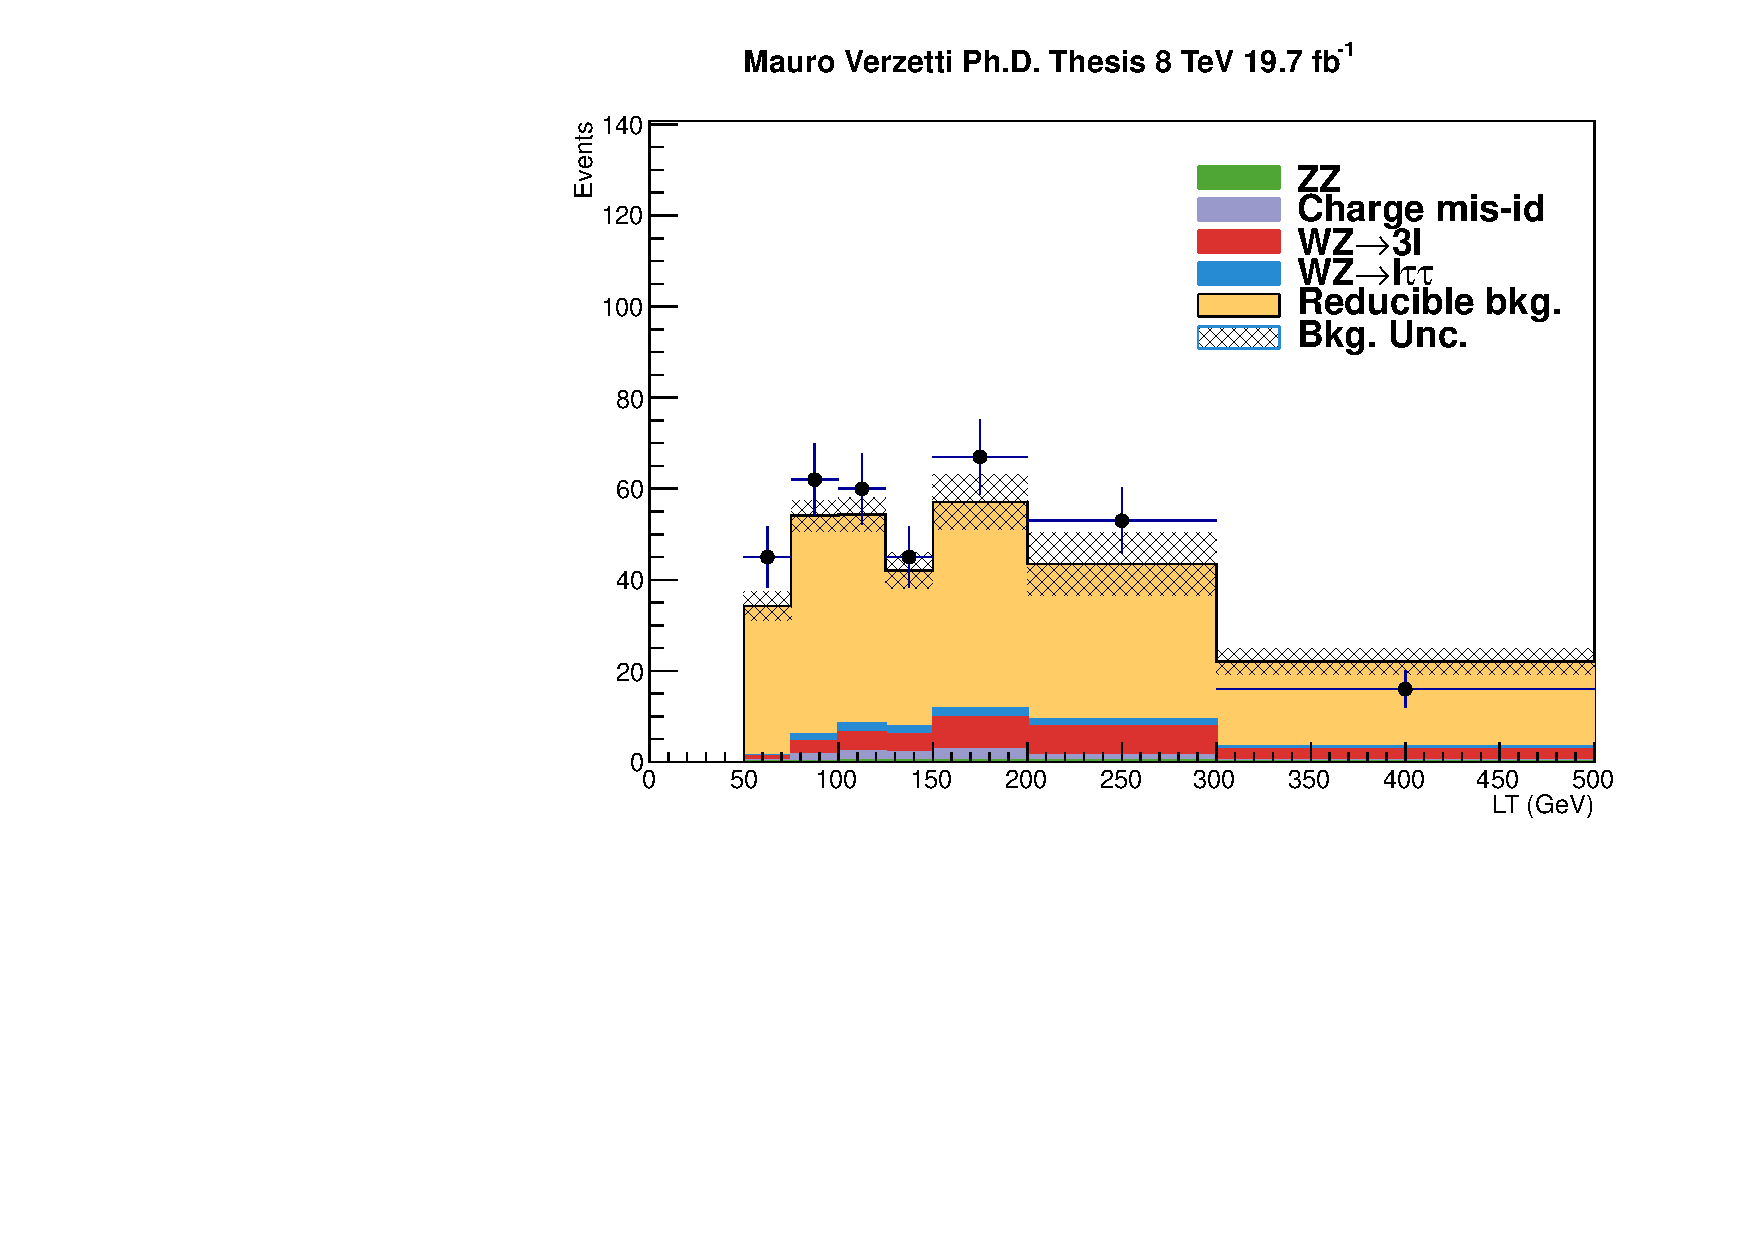
\includegraphics[width=0.49\textwidth]{4_Analisys/pics/8TeV/plots/emt/f3/final-f3-LT-charge3.pdf}\\
  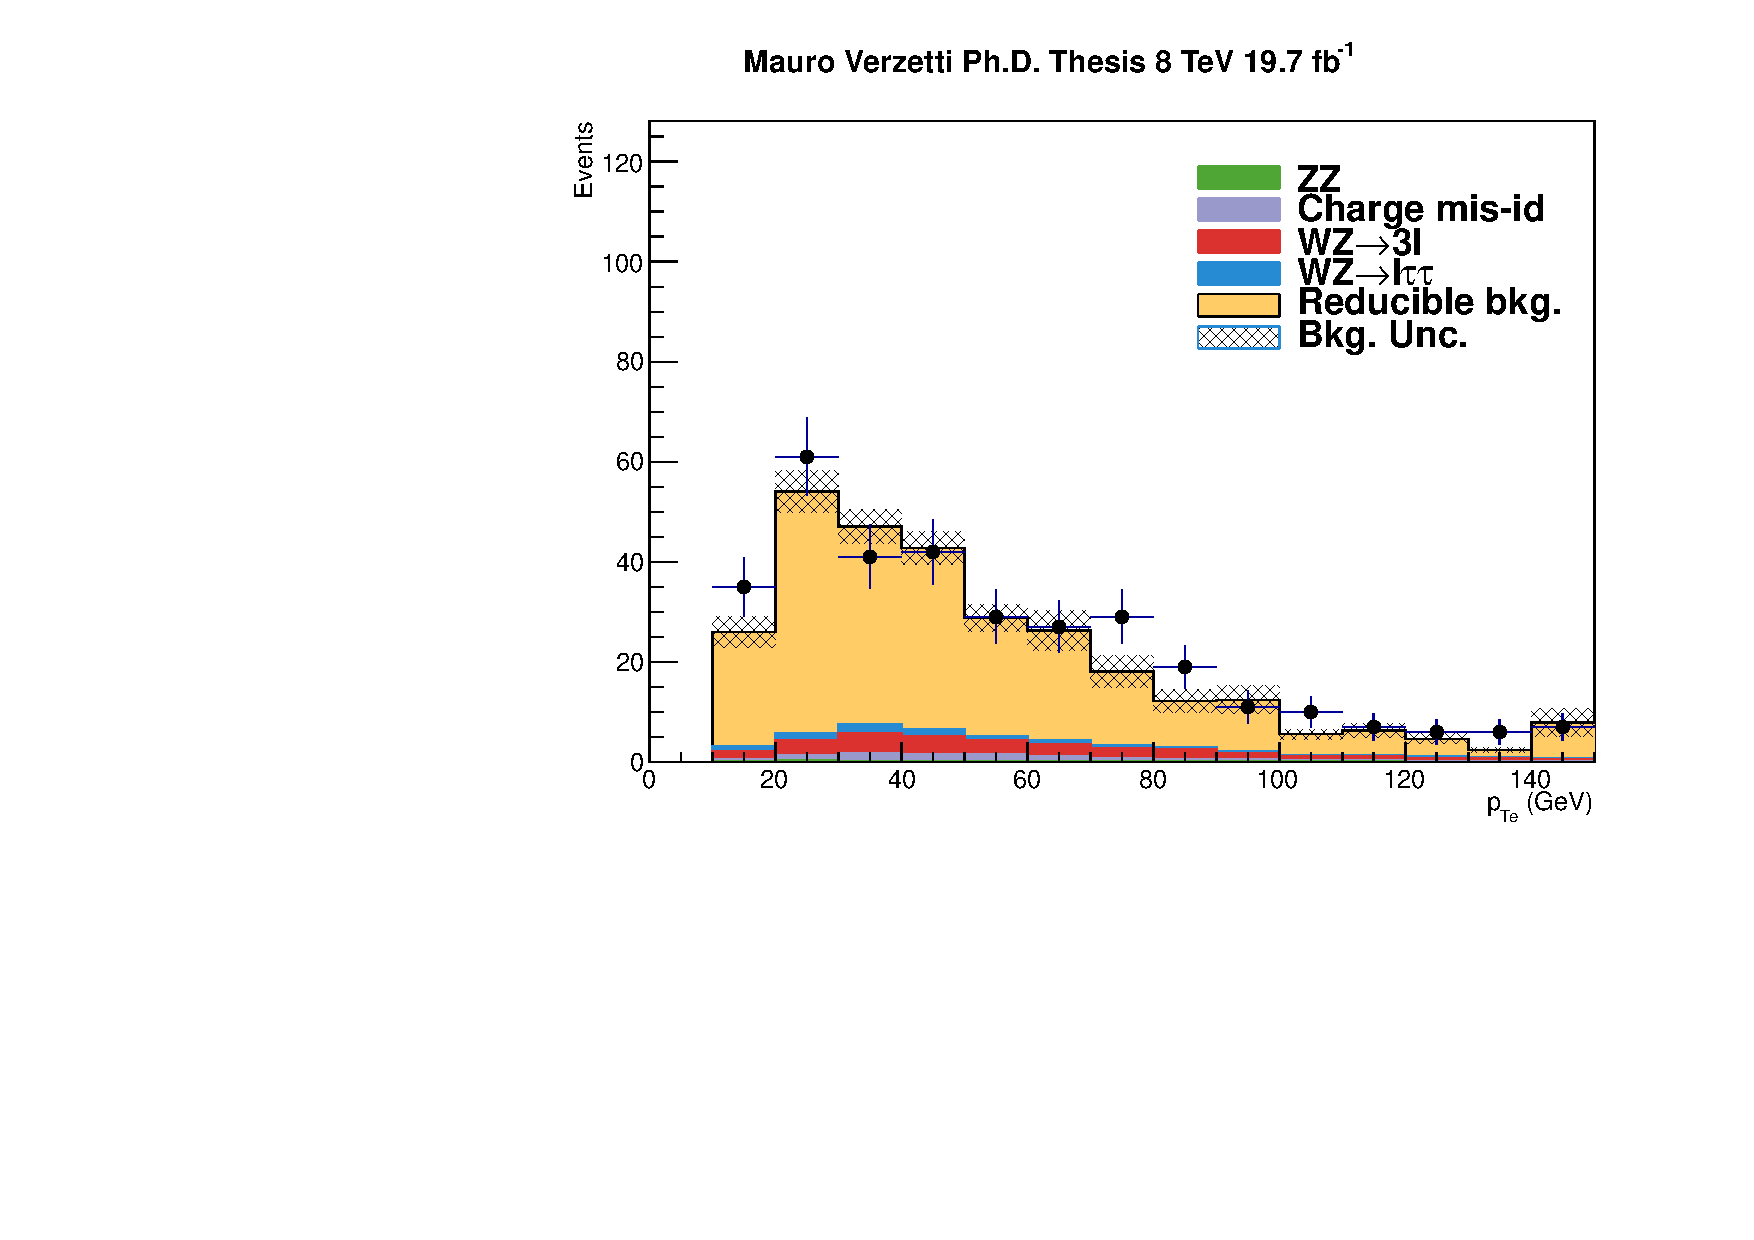
\includegraphics[width=0.49\textwidth]{4_Analisys/pics/8TeV/plots/emt/f3/Full_charge3/final-f3-ePt-Full.pdf}
  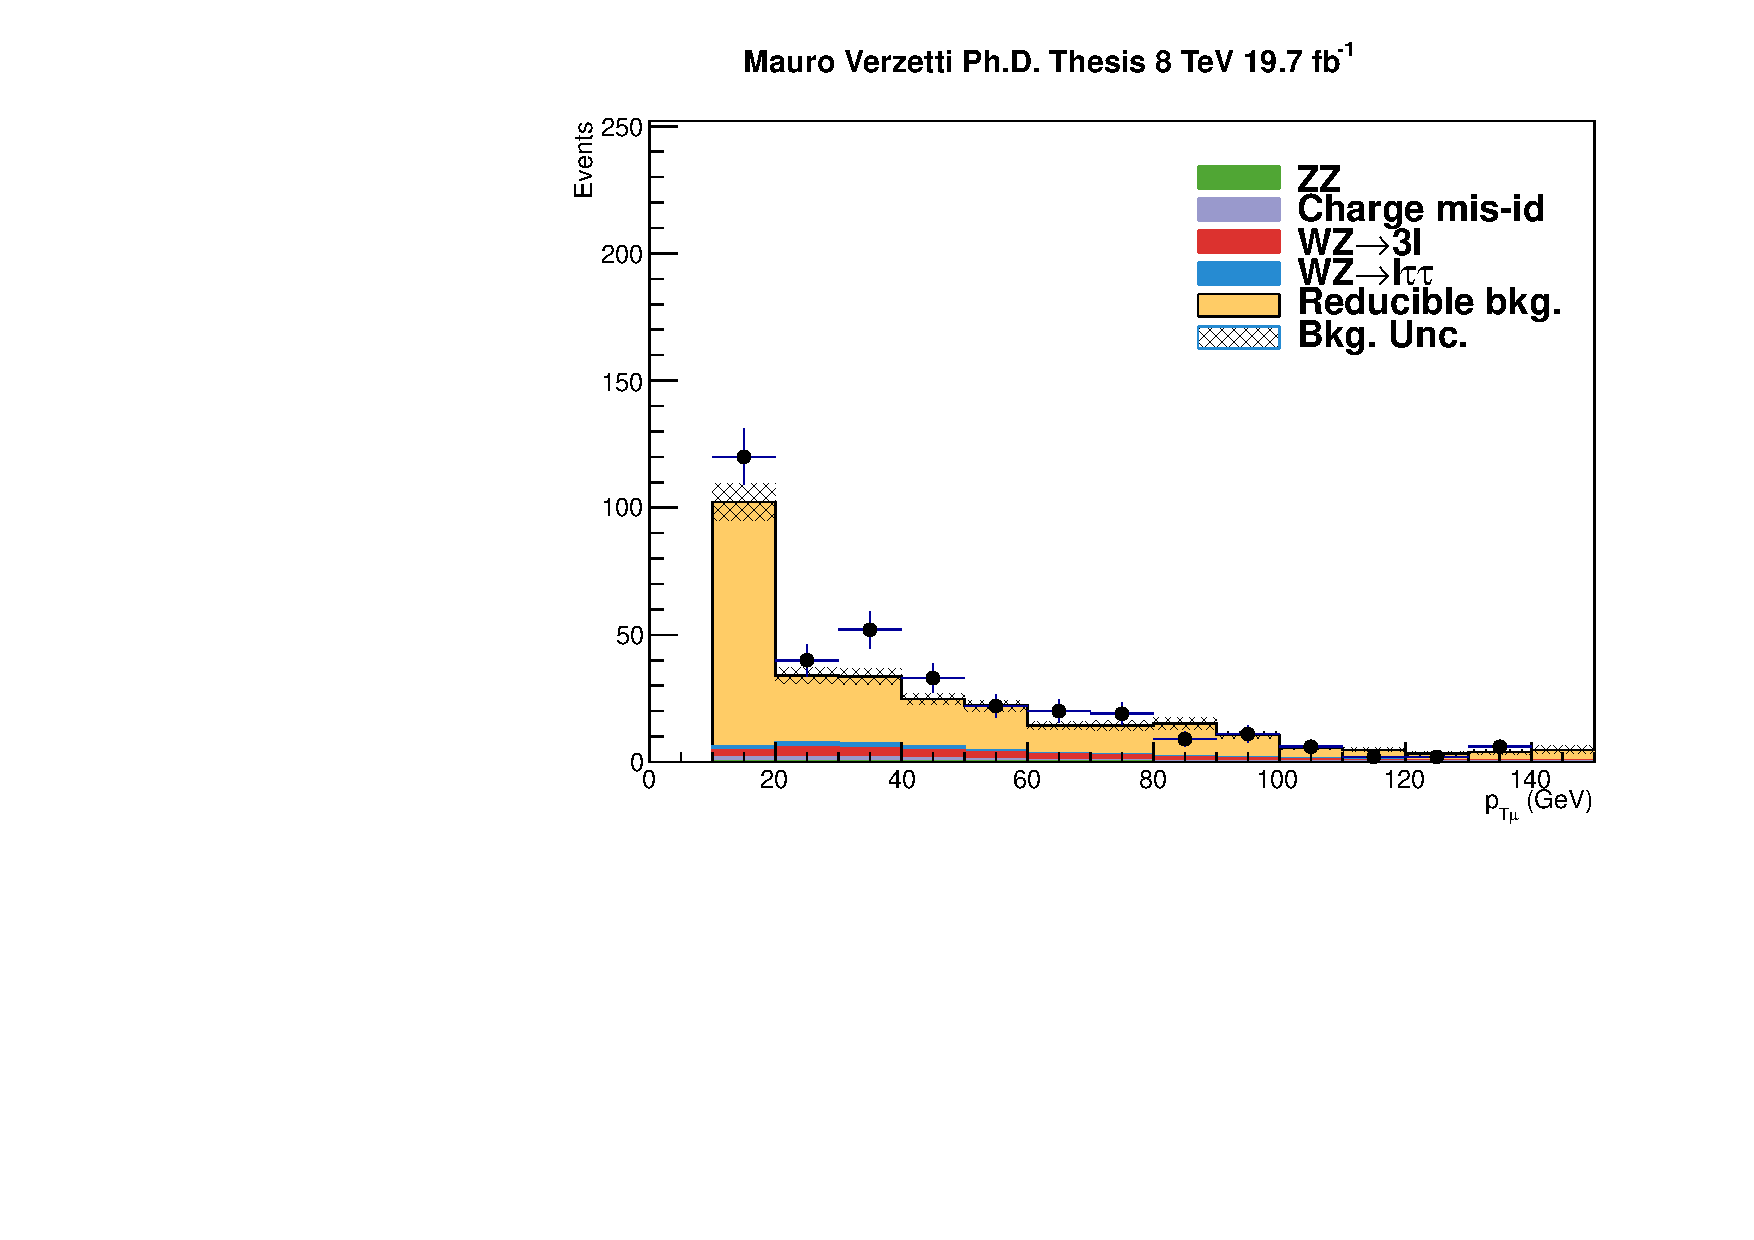
\includegraphics[width=0.49\textwidth]{4_Analisys/pics/8TeV/plots/emt/f3/Full_charge3/final-f3-mPt-Full.pdf}\\
  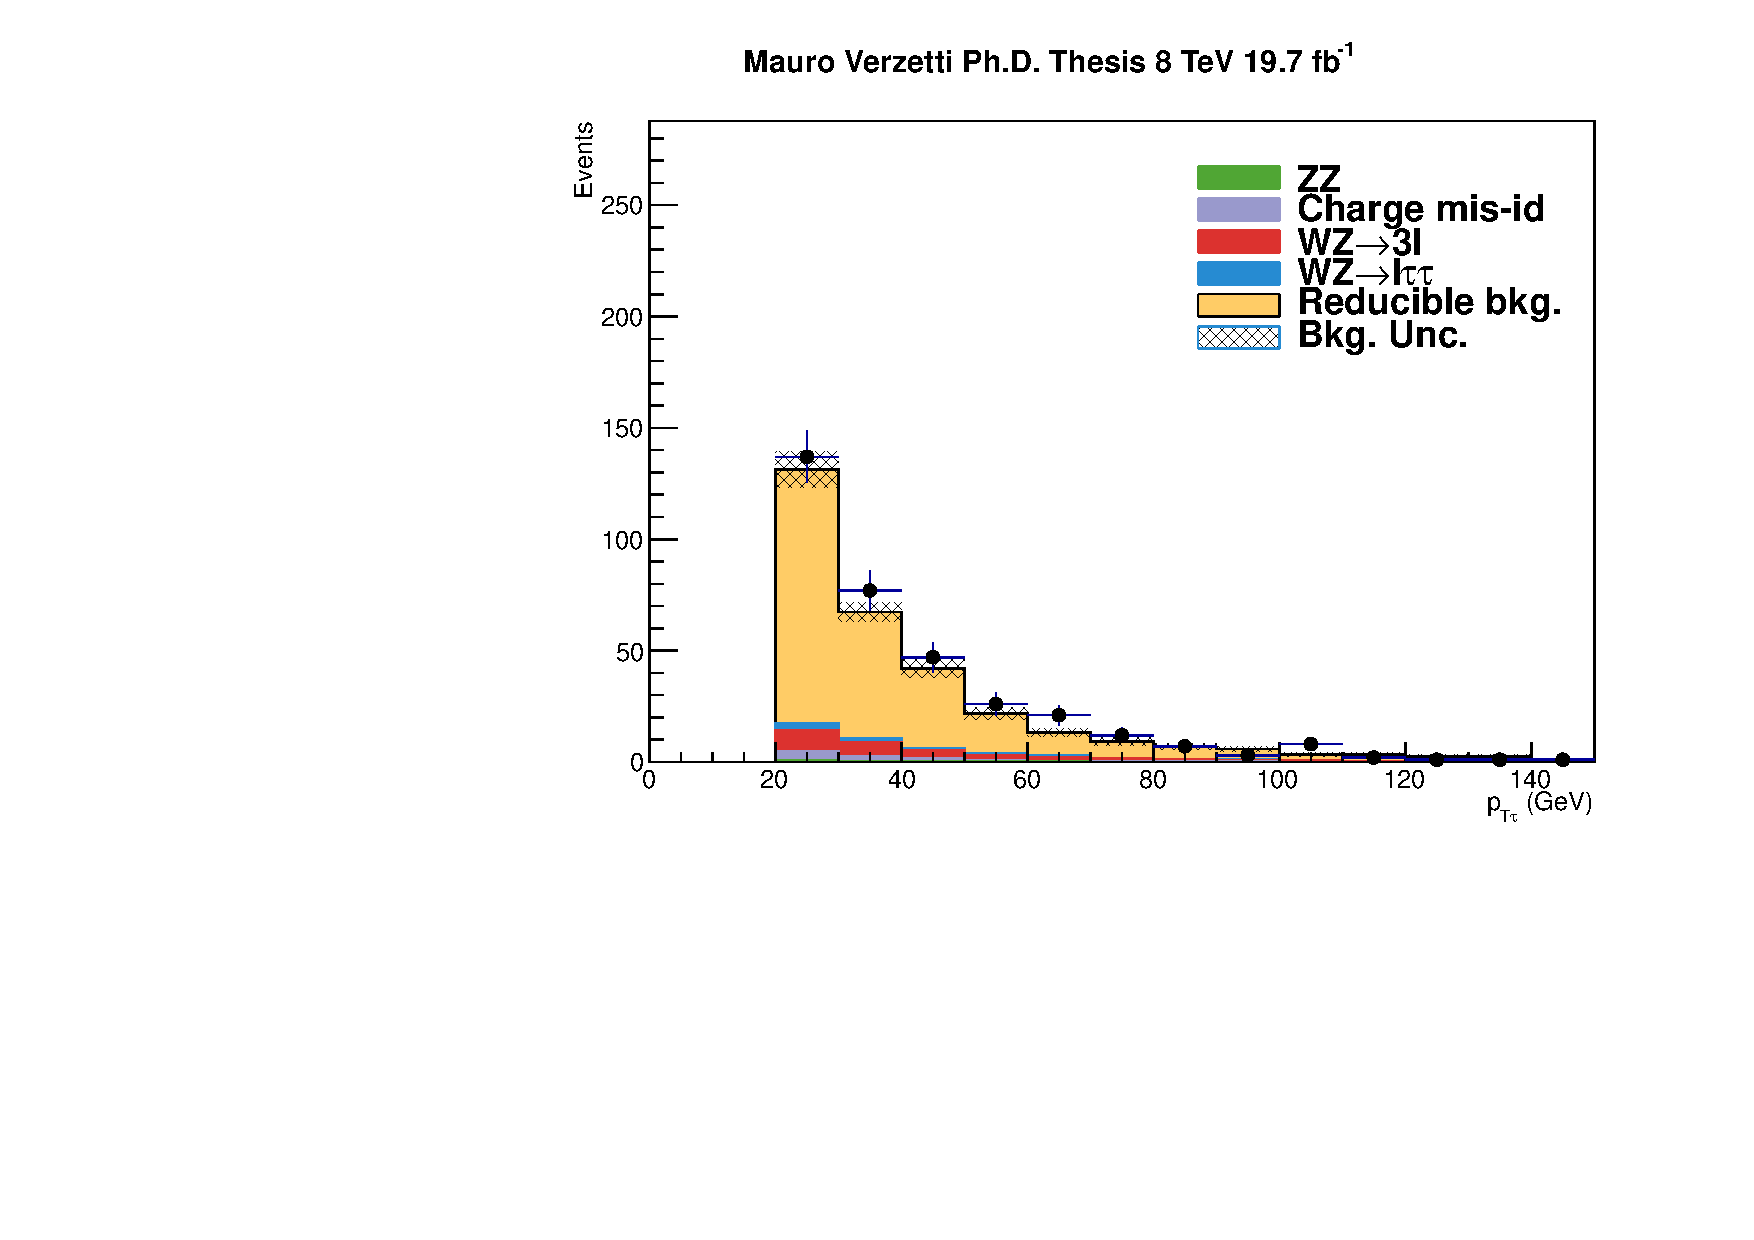
\includegraphics[width=0.49\textwidth]{4_Analisys/pics/8TeV/plots/emt/f3/Full_charge3/final-f3-tPt-Full.pdf}
  \caption{Comparison of measured and predicted backgrounds in the $e\mu\tau_h$ ``fake tau, charge $\pm3$'' control region for 8 TeV data.
  From top left to bottom: mass of the sub-leading lepton and the tau system, scalar sum of the leptons \pT ($L_T$), \pT of the electron, muon, and hadronic tau.
  The reducible background contribution is estimated by the kNN method, in the same manner as in the signal region.
  The shaded band represents the uncertainty on the sum of the background contributions.
  }
  \label{fig:LLT_emt_f3_charge3_control_8TeV}
\end{center}
\end{figure}


\begin{figure}
\begin{center}
  \includegraphics[width=0.49\textwidth]{4_Analisys/pics/7TeV/plots/eet/f3/Full_charge3/final-f3-subMass-Full.pdf}
  \includegraphics[width=0.49\textwidth]{4_Analisys/pics/7TeV/plots/eet/f3/final-f3-LT-charge3.pdf}\\
  \includegraphics[width=0.49\textwidth]{4_Analisys/pics/7TeV/plots/eet/f3/Full_charge3/final-f3-e1Pt-Full.pdf}
  \includegraphics[width=0.49\textwidth]{4_Analisys/pics/7TeV/plots/eet/f3/Full_charge3/final-f3-e2Pt-Full.pdf}\\
  \includegraphics[width=0.49\textwidth]{4_Analisys/pics/7TeV/plots/eet/f3/Full_charge3/final-f3-tPt-Full.pdf}
  \caption{Comparison of measured and predicted backgrounds in the $ee\tau_h$ ``fake tau, charge $\pm3$'' control region for 7 TeV data.
  From top left to bottom: mass of the sub-leading electron and the tau system, scalar sum of the leptons \pT ($L_T$), \pT of the leading and sub-leading electron, and \pT of the hadronic tau.
  The reducible background contribution is estimated by the kNN method, in the same manner as in the signal region.
  The shaded band represents the uncertainty on the sum of the background contributions.
  }
  \label{fig:LLT_eet_f3_charge3_control_7TeV}
\end{center}
\end{figure}

\begin{figure}
\begin{center}
  \includegraphics[width=0.49\textwidth]{4_Analisys/pics/8TeV/plots/eet/f3/Full_charge3/final-f3-subMass-Full.pdf}
  \includegraphics[width=0.49\textwidth]{4_Analisys/pics/8TeV/plots/eet/f3/final-f3-LT-charge3.pdf}\\
  \includegraphics[width=0.49\textwidth]{4_Analisys/pics/8TeV/plots/eet/f3/Full_charge3/final-f3-e1Pt-Full.pdf}
  \includegraphics[width=0.49\textwidth]{4_Analisys/pics/8TeV/plots/eet/f3/Full_charge3/final-f3-e2Pt-Full.pdf}\\
  \includegraphics[width=0.49\textwidth]{4_Analisys/pics/8TeV/plots/eet/f3/Full_charge3/final-f3-tPt-Full.pdf}
  \caption{Comparison of measured and predicted backgrounds in the $ee\tau_h$ ``fake tau, charge $\pm3$'' control region for 8 TeV data.
  From top left to bottom: mass of the sub-leading electron and the tau system, scalar sum of the leptons \pT ($L_T$), \pT of the leading and sub-leading electron, and \pT of the hadronic tau.
  The reducible background contribution is estimated by the kNN method, in the same manner as in the signal region.
  The shaded band represents the uncertainty on the sum of the background contributions.
  }
  \label{fig:LLT_eet_f3_charge3_control_8TeV}
\end{center}
\end{figure}



